\documentclass[12pt]{article}
\usepackage[margin=1in]{geometry}
\usepackage{amsmath}
\usepackage{amssymb}
\usepackage{graphicx}
\usepackage{booktabs}
\usepackage{xurl}
\usepackage[hidelinks]{hyperref}

\setlength{\tabcolsep}{3pt}
\emergencystretch=3em

\newcommand{\FDL}{\textnormal{[proved/checked finite-dimensional]}}
\newcommand{\CND}{\textnormal{[conditional]}}
\newcommand{\OBS}{\textnormal{[observed numerical evidence]}}
\newcommand{\OPN}{\textnormal{[open conjecture]}}
\newcommand{\CTX}{\textnormal{[counterexample]}}

\title{Pose-Confounding Spectral Geometry for Full-Wave Inverse-Scattering SLAM:
An Executable Finite-Dimensional Study}
\author{Inv-SLAM idea-loop experiment synthesis (executable-record draft)}
\date{2026-09-04}

\begin{document}

\maketitle

\begin{abstract}
We study local observability of a volumetric material-contrast map when the
transmitting and receiving platform pose is unknown. A two-dimensional scalar
Helmholtz contrast-source model yields whitened and realified map and pose
Jacobians $A$ and $B$. Eliminating pose gives the no-prior information
$K_{\mathrm{SLAM}}=A^T P_{\mathrm{Range}(B)^\perp}A$ and, with a positive pose
prior, a Schur complement $K_{\mathrm{eff}}$. Finite-dimensional identities
link exact ambiguity to $\mathrm{Range}(A)\cap\mathrm{Range}(B)$, identify the
no-prior generalized retention spectrum with squared sines of principal
angles, and bound the information defect by $\mathrm{rank}(B)$.

An executable synthetic harness checks the self-cell quadrature, analytic map
and pose derivatives, whitening, Schur identities, gauge directions,
frequency stacking, trajectory perturbations, and generalized-eigenvalue
derivatives. Its falsifiers materially narrow the claims: a proposed universal
trajectory ordering holds in 0/24 replicated cells; raw and normalized
orderings agree in only 2/12 scene--frequency cells; an apparent ring-scene
rank failure is caused by squaring a near-null singular value and applying a
machine-rank threshold; and full nonlinear robustness remains sampled evidence,
not a certificate. A fixed-true-pose Monte Carlo experiment also targets a
frequentist sandwich covariance rather than the Bayesian marginal
$K_{\mathrm{eff}}^{-1}$.

A complete Born control supplies a sharper limiting result. For
$F_B(\chi,X)=A_0(X)\chi$ and $\chi=s\bar\chi$, the exact discrete tangents obey
$A_B(s)=A_0$ and $B_B(s)=sB_1$. Consequently, for every $s\ne0$ the no-prior
pose projector and $K_{\mathrm{SLAM}}$ are amplitude-invariant, whereas at
$s=0$ one has $B_B=0$ and $K_{\mathrm{SLAM}}=K_{\mathrm{IS}}$; with a strictly
positive prior the information loss is instead $O(s^2)$. This rank-stratum
singularity explains why a no-prior normalized metric can remain confounded as
the physical pose signal vanishes. All results are local and
finite-dimensional on the recorded 2D scalar grids; no continuum transfer,
global recovery, real-data performance, or priority claim is made.
\end{abstract}

\tableofcontents

\section{Introduction and contributions}\label{sec:intro}

Simultaneous localization and mapping (SLAM) from coherent full-wave
measurements couples a map of material contrast to the unknown poses at which
the scene is probed. When the underlying forward model is a nonlinear inverse
scattering map, the standard information-theoretic reduction first linearizes
about a nominal contrast and trajectory, whitens the measurement noise, and
realifies the parameters so that real pose increments act on real degrees of
freedom. Eliminating the pose nuisance then produces an effective
map-information operator whose local geometry can be characterized by
finite-dimensional linear algebra.

The contribution of this draft is deliberately bounded:
\begin{itemize}
\item We formulate and test an explicit finite-dimensional theory in which
the pose-induced information loss is low rank, the no-prior normalized
retention spectrum equals the squared-sine principal-angle spectrum between
the map and pose data tangents, and finite-prior retention is a weighted
Schur-complement shrinkage. These statements are elementary and are labelled
\FDL{}; they are verified on the discrete harness recorded here, not on the
continuum problem.
	\item We execute the round-1, round-2, and round-3 experiment families and
controls on one Apple Silicon CPU harness with deterministic seeds,
machine-precision rank tolerances, exact commands, hashes, and raw JSON
records, and we keep the failures and counterexamples exactly as recorded
(Sections~\ref{sec:results} and Appendix~\ref{app:claims}). The round-2
results appear in Sections~\ref{sec:family6}--\ref{sec:family5b2}; the
round-3 results and parent extension appear in
Sections~\ref{sec:family10}--\ref{sec:family15b}.
\item We isolate a weak-scattering semantic trap. The complete Born tangent
pair satisfies $A_B(s)=A_0$ and $B_B(s)=sB_1$: normalized no-prior confounding
is constant on each nonzero-amplitude rank stratum but jumps at $s=0$, while a
strictly positive pose prior regularizes the loss to $O(s^2)$
(Section~\ref{sec:family15b}).
\item We state the boundary explicitly: no continuum transfer, global
nonlinear convergence, online SLAM performance, or global novelty is claimed
(Section~\ref{sec:limits}), and all full nonlinear execution-error robustness
statements are demoted to empirical/structural observations
(Section~\ref{sec:family14}). Retrieval-bounded related work is discussed in
Section~\ref{sec:related}; this draft makes no priority claim.
\end{itemize}

All matrix identities below are stated in the whitened/realified data space
with real map and pose parameters. The results are local and information-
theoretic; they concern local observability and Fisher-type information, not
estimation, recovery, or decision performance.

\section{Model, whitening/realification, and information operators}\label{sec:model}

\subsection{Discrete contrast-source model}

The scenario is a deterministic, synthetic two-dimensional scalar Helmholtz
contrast-source problem on $D=[-0.5,0.5]^2$ discretized on a uniform $N\times
N$ grid with step $h=1/N$. Let $k_b$ be the background wavenumber and
$\chi$ the relative contrast
\[
\chi(r)=\frac{k^2(r)-k_b^2}{k_b^2},
\]
so that the contrast is dimensionless. The free-space Green function is
\[
g_k(r,r')=\frac{i}{4}H_0^{(1)}(k_b|r-r'|),
\]
with gradient convention
\[
\nabla_r g_k(r,r')=-\frac{i k_b}{4}H_1^{(1)}(k_b R)\frac{r-r'}{R},\qquad
R=|r-r'|.
\]
For the equal-area disk cell of radius $a=h/\sqrt{\pi}$, the domain-propagator
diagonal uses the complete disk integral \FDL{} (corrected 2026-09-03, see
Section~\ref{sec:family1}):
\[
I_{\mathrm{self}}=\frac{i\pi a}{2k_b}H_1^{(1)}(k_b a)-\frac{1}{k_b^2},\qquad
[G_D]_{nn}=k_b^2 I_{\mathrm{self}}.
\]
The linearized state operator is $M_t=I-D_\chi G_{D,t}$ with the total field
defined through the contrast-source Lippmann--Schwinger equation, and the
current-eliminated forward map is $F(\chi,X)=G_S M^{-1} D_\chi E^{\mathrm{inc}}$
for a trajectory $X=(x_1,\ldots,x_T)$ of poses $x_t=(p_x,p_y,\theta)\in
\mathrm{SE}(2)$.

\subsection{Whitening and realification}

For a covariance model with whitening factor $W$, the complex-valued Jacobians
are converted to real matrices of doubled row count,
\[
A_R=\sqrt{2}\begin{bmatrix}\Re(WA)\\\Im(WA)\end{bmatrix},\qquad
B_R=\sqrt{2}\begin{bmatrix}\Re(WB)\\\Im(WB)\end{bmatrix},
\]
where $A=D_\chi F$ is the map Jacobian and $B=D_X F$ is the pose Jacobian.
All projectors, ranks, principal angles, Schur complements, and spectra in
this draft are computed after this conversion. Complex-linear projectors
$BB^+$ acting on real pose increments would enlarge the nuisance range and
overestimate map--pose confounding; they are not used. In the executed runs
$W$ is the identity ($W=I$) except where a declared block-normalization or
SNR-matched control rescales rows per frequency block.

\subsection{Information operators}

In the whitened/realified space, with $m$ real data rows and $q$ real pose
columns, define the known-pose map information, the no-prior pose-eliminated
information, and the finite-prior Schur complement by
\begin{align}
K_{\mathrm{IS}}&=A^T A,\\
K_{\mathrm{SLAM}}&=A^T P_{\mathrm{Range}(B)^\perp}A
=A^T(I-BB^+)A,\\
K_{\mathrm{eff}}(\alpha)&=A^TA-A^TB\,(B^TB+\alpha I)^{-1}B^TA,
\qquad \alpha>0,
\end{align}
where the $q\times q$ system is solved stably. At $\alpha=0$ the displayed
inverse is valid only when $B$ has full column rank; in general the no-prior
operator is defined separately by the orthogonal projector $I-BB^+$ above.
The pose-induced loss is
$L_X=K_{\mathrm{IS}}-K_{\mathrm{eff}}$. For no prior the generalized retention
spectrum is obtained from $Q_A^T P_{\mathrm{Range}(B)^\perp}Q_A$ with
orthonormal bases $Q_A$ and $Q_B$ of $\mathrm{Range}(A)$ and
$\mathrm{Range}(B)$: with descending singular values of $Q_B^TQ_A$, the
retentions are reported in ascending order as
\[
\rho_i=1-\sigma_i^2(Q_B^TQ_A),
\]
padded with $\rho_i=1$ in unmatched directions. This is the
\FDL{} identity $K_{\mathrm{SLAM}}v=\rho K_{\mathrm{IS}}v$ on the observable
support of $K_{\mathrm{IS}}$ expressed through principal angles.

The executed algebraic statements, all \FDL{}, are:
\begin{enumerate}
\item $\ker K_{\mathrm{SLAM}}=\{u: Au\in \mathrm{Range}(B)\}$ (including
$\ker A$).
\item $\mathrm{rank}\,K_{\mathrm{IS}}-\mathrm{rank}\,K_{\mathrm{SLAM}}=
\dim(\mathrm{Range}(A)\cap\mathrm{Range}(B))$.
\item $0\le K_{\mathrm{SLAM}}\le K_{\mathrm{IS}}$, and at most
$\mathrm{rank}(B)$ generalized retention values differ from $1$.
\item $\mathrm{rank}\,L_X\le \mathrm{rank}(B)$, with Hermitian interlacing
between $K_{\mathrm{IS}}$, $K_{\mathrm{eff}}(\alpha)$, and $K_{\mathrm{SLAM}}$.
\item Along a fixed-rank regular path $J_X=\alpha I$, $K_{\mathrm{eff}}\to
K_{\mathrm{SLAM}}$ as $\alpha\to0$ and $K_{\mathrm{eff}}\to K_{\mathrm{IS}}$
as $\alpha\to\infty$, on the tested support. A singular-support prior (an
unpenalized pose direction) prevents convergence to $K_{\mathrm{IS}}$
(\CND{} + \FDL{} on the recorded finite geometry).
\item Duplicating data as $A_{\mathrm{aug}}=[A;cA]$,
$B_{\mathrm{aug}}=[B;cB]$ scales $K_{\mathrm{IS}}$ and $K_{\mathrm{SLAM}}$ by
$1+c^2$ and leaves the no-prior retentions unchanged; with a fixed finite
prior the data-to-prior weighting changes and retentions generally move; a
jointly scaled prior $J_X^{\mathrm{aug}}=(1+c^2)J_X$ restores invariance.
\end{enumerate}

For a full-wave model at zero background $\chi_0=0$, the first-order pose
Jacobian vanishes ($B=0$) so $K_{\mathrm{SLAM}}=K_{\mathrm{IS}}$; pose effects
then first appear through the bilinear term $(D_X A[\delta X])\delta\chi$,
which the runs evaluate rather than declare harmless.

\section{Experiment design}\label{sec:design}

\subsection{Unified harness and scenario}

One deterministic harness in \texttt{src/} implements the forward model, the analytic
Jacobian builders, whitening/realification, and the algebraic checks. The
nominal scene is the two-Gaussian contrast
$\chi_0=0.3\,\chi_{\mathrm{disk},1}+0.5\,\chi_{\mathrm{disk},2}$ used by
Family~1 with centers $(-0.15,-0.12)$ and $(0.18,0.14)$, widths
$\sigma=(0.09,0.07)$; $k_b=2\pi$; $T=6$ poses; and $n_{\mathrm{rx}}=4$
body-fixed receivers per pose, giving $m=48$ real data rows and $q=18$ pose
columns after realification. The pilot grid is $N=16$; N=24/32/40 runs are
recorded as refinement diagnostics. Two map parameterizations are analyzed:
the $N^2$-column pixel basis and a $p=24$ smooth Gaussian-RBF basis with unit
columns (4$\times$6 lattice, $\sigma_b=0.16$).

\subsection{Five families and parent corrections}

\begin{enumerate}
\item Family 1 verifies the corrected self-cell rule, direct radial
quadrature, source-gradient sign, centered map/pose finite differences, state
margin, Born/full-wave continuation, and a forward-model grid-refinement
diagnostic.
\item Family 2 checks the kernel/rank/retention identities, loss rank and
interlacing, prior sweeps, singular-prior limits, duplicate-block rules, and
smooth-basis resolution persistence. Parent corrections added a stable
$C^TC$ factorization check and an SVD-filtered small-prior sweep.
\item Family 3 tests smooth-basis and pixel-basis SE(2) gauge cancellation,
kernel distances, anchor/symmetry controls, and Born-empty-background
degeneration. Family 3b reruns the same claims under corrected validity
conditions (generator-representing augmented basis, generator-specific
retention, and genuinely small scene amplitudes) without modifying the raw
Family 3 record.
\item Family 4 stacks genuinely distinct frequency blocks with one shared
pose compensation, checks PSD monotonicity and duplicate controls, and
compares four equal-budget trajectories. Family 4b adds a declared
block-normalized control; the parent controls add an SNR-matched frequency
control and equal-length/same-radius trajectory orderings.
\item Family 5 verifies full trajectory/eigenvalue derivative formulas against
finite differences, quantifies the frozen-nuisance error, tests a robust
first-order surrogate, records an empirical-only Weyl/Lipschitz self-check,
and scans a random path for near-crossings and rank events.
\end{enumerate}

\paragraph{Round-2 families and their roles.}
\begin{itemize}
\item Family 6 declares a per-frequency colored-noise covariance with a
receiver Mat\'ern-1/2 factor and per-frequency SNR-matched whitening, and
reruns whitening sanity, algebraic-spine, duplicate-block, and stacking
checks under the declared colored-whitened blocks (colored-noise control).
\item Family 4c holds curved-path standoff fixed and equalizes each pose's
realified $A$-block energy before projection, so trajectory geometry is
compared after removing radius/standoff and per-pose signal-strength scaling
(trajectory and standoff control).
\item Family 7 records resolution, frequency-rank, near-crossing, and
Born-to-full-wave contrast diagnostics on finite grids (continuum/rank
diagnostics only, not a continuum proof).
\item Family 8 makes the current-space $G_S$/SOM and map-tangent
$A$/$K_{\mathrm{eff}}$ objects explicit in the same pixel space and checks
their composition identity, range containment, and mode-subspace distinction
(SOM/current-space distinction).
\item Family 9 reruns the algebraic-spine and frequency-diversity claims over
seven scenes and records pose-DOF, receiver-count, pose-count, and
smooth-basis ablations (replications and component ablations).
\item Family 5b2 derives an alpha-aware structural operator-Lipschitz bound
for the affine tangent model and verifies the certificate on 2000 directions;
the loose Family 5b precursor is cited only as corrected by Family 5b2
(Lipschitz certification).
\end{itemize}

\paragraph{Round-3 families and their parent extension.}
\begin{itemize}
\item Family 10 reruns the finite-dimensional NLS covariance toy and records
the protocol correction for its fixed-true-pose Monte Carlo scheme: the
correct linearized frequentist target is the sandwich covariance
$P_{\mathrm{samp}}$, not the Bayesian marginal $K_{\mathrm{eff}}^{-1}$; the
original comparison is retained as a protocol-correction/negative result
(protocol-corrected online-NLS-toy comparison).
\item Family 11 replicates the non-monotone SNR dependence and finite
high-SNR plateau of the frequency-diversity movements across three scenes and
two second frequencies, and records equal-SNR frequency-set growth,
duplicate-block invariance under the jointly scaled prior, and a
fixed-count bandwidth sweep (SNR/frequency-set replication).
\item Family 12 replicates the Family-4/4c trajectory comparison over four
scenes, two controls, and three frequency sets, records cross-checks against
the stored Family 4c and Family 4 artifacts, and documents which scene,
frequency-set, control, and geometry changes move the ranking (trajectory
replication and mechanism).
\item Family 13 autopsies the Family-9 ring-scene machine-rank boundary with
predeclared relative-tolerance grids, stable/effective-rank diagnostics, and
backward residuals, and decides between a discontinuous rank change,
tolerance classification, and unstable subtraction (rank-boundary autopsy).
\item Family 14 audits the robustness scope of the stored Family 5b/5b2 and
generalized-derivative evidence, recomputes the affine certificate rows, and
demotes all full nonlinear execution-error robustness claims to
empirical/structural observations (robustness-scope demotion).
\item Family 15 checks the self-derived Born map identity
$A_{\mathrm{Born}}=G_S\,\mathrm{diag}(E^{\mathrm{inc}})$, records
Born-versus-full-wave relative deviations while deliberately sharing the
full-wave pose block $B_{\mathrm{full}}$, and compares the structure with the
Diong et al.\ Born/CRB study. These rows are a mixed-tangent isolation
control, explicitly not a complete Born-SLAM model or external benchmark.
\item Family 15b constructs and finite-difference checks the analytic Born pose
Jacobian $B_B$, compares complete pairs $(A_B,B_B)$, and tests the exact
nonzero-scale projector invariance, the singular $s=0$ endpoint, and the
finite-prior $O(s^2)$ loss bound (complete Born pose-tangent control).
\end{itemize}

\subsection{Tolerances, seeds, and environment}

Rank tolerance for exact algebraic checks is
$\tau(M)=\max(m,n)\,\epsilon_{\mathrm{machine}}\,\sigma_1(M)$. PSD and
interlacing violations are rejected above
$-10^{-10}\max(1,\|K_{\mathrm{IS}}\|_2)$; the c1 subspace gate is
$10^{-8}\max(1,\|A\|_2^2)$; c3 prediction residual gate is
$10^{-10}\max(1,\|A\|_2^2)$; c8 invariance gates are $10^{-10}$. Deterministic
seeds are recorded per run (map seeds $\{0,1,2\}$, pose seeds
$\{10,11,12\}$, gauge Born seed 31415, Family 5 perturbation seeds
2718/9191/150 samples, etc.). All runs execute on Apple Silicon CPU only
(macOS-26.6.2 arm64), Python 3.12.13, numpy 2.5.2, scipy 1.18.1, matplotlib
3.11.1; no GPU/MPS/CUDA, no network services, and no random draws except the
declared fixed seeds.

\section{Results}\label{sec:results}

Each subsection reports the key numbers from the recorded JSONs followed by
the preserved negative results and counterexamples. Statuses are quoted
exactly as executed; Appendix~\ref{app:claims} repeats the claim-status
tables. Figure files produced by the runs are listed in the reproducibility
section.

\subsection{Round-3 scope layering}\label{sec:scope-layering}

Every Round-3 claim below belongs to exactly one of four layers; the layer is
the scope statement, and no result moves between layers unless the demotion in
Section~\ref{sec:family14} explicitly says so.
\begin{enumerate}
\item \emph{Exact finite-dimensional linear algebra.} Rank, retention,
principal-angle, and kernel identities for the recorded whitened/realified
Jacobian pairs, together with the affine tangent certificate of
Section~\ref{sec:family5b2}, are statements about exact linear algebra on the
discrete matrices and are labelled \FDL{}.
\item \emph{Conditional/discretized full-wave differentiation.}
FD-validated Jacobians are finite-difference checks of the implemented
discrete model only. They numerically support the analytic derivative
implementation, conditional on the discretization and the recorded numerical
floors; they do not certify a continuum derivative.
\item \emph{Executed numerical evidence and preserved counterexamples.} The
recorded results and preserved negatives are empirical statements on the
tested scenario: the trajectory-ordering hypothesis is false (0/24 cells), the
ring machine-rank boundary is a tolerance classification, the SNR/frequency
diversity curve is non-monotone with a scene-specific exception, Born and
full-wave operators deviate beyond weak scattering, and the online-toy
fixed-pose covariance does not match its linearized sandwich target at 120
trials. Such rows are labelled \OBS{} or \CTX{} and are not relabelled.
\item \emph{Open continuum, nonlinear-global, real-system, and novelty
questions.} No interval/uniform nonlinear certificate, no 3D/vector
extension, no real data, and no continuum transfer are established; the
429-limited novelty search is a retrieval limitation, not a novelty verdict.
These remain \OPN{}.
\end{enumerate}

\subsection{Family 1: forward model and corrected analytic Jacobians}\label{sec:family1}

The initial Family-1 implementation used an invented self-cell rule that
omitted the lower endpoint of the Hankel antiderivative
($\lim_{x\to0}xH_1^{(1)}(x)=-2i/\pi$), so the alleged disk integral tended to
$1/k_b^2$ instead of zero as $h\to0$. The pre-correction snapshot is preserved
verbatim under \texttt{archive/INVALIDATED\_self\_cell\_2026-09-03T092339Z/}. The
corrected rule
$I_{\mathrm{self}}=i\pi a H_1^{(1)}(k_ba)/(2k_b)-1/k_b^2$ matches 2048-node
radial quadrature to max absolute error $3.13\times10^{-16}$, with
$|I_{\mathrm{self}}|$ dropping monotonically from $5.12\times10^{-3}$
(N=8) to $4.36\times10^{-5}$ (N=128); the invalidated rule stays near
$2.5\times10^{-2}$. The source-gradient identity
$\nabla_s g=-\nabla_z g$ is unit-tested against finite differences in the
source coordinate (corrected relative error $1.7\times10^{-9}$ versus
$2.0$ for the old sign).

\begin{table}[ht]
\centering
\small
\caption{Family 1 key numbers (recorded in
\texttt{results/family1\_pilot\_results.json} and
\texttt{results/family1\_grid\_refinement.json}).}
\label{tab:f1}
\begin{tabular}{p{0.38\textwidth} p{0.54\textwidth}}
\toprule
quantity & value \\
\midrule
map-FD rel.\ error at h=$10^{-3}$ (seeds 0/1/2) &
$2.25\times10^{-9}$ / $1.74\times10^{-8}$ / $1.77\times10^{-9}$ \\
pose-FD rel.\ error at h=$10^{-3}$ (seeds 10/11/12) &
$8.38\times10^{-7}$ / $4.28\times10^{-6}$ / $4.09\times10^{-6}$ \\
map slope / pose slope (5-pt window) &
1.976 (r$^2$=0.9998) / 2.0000 (r$^2$=1.0000) \\
state margin $\sigma_{\min}(M)/\|M\|_2$; max residual &
0.7189; $9.34\times10^{-16}$ \\
Born/full-wave rel.\ discrepancy, s=0.01..0.2 &
F: $1.77\times10^{-3}$..$3.54\times10^{-2}$; A-Fro: $1.89\times10^{-3}$..$3.82\times10^{-2}$ \\
grid rel.\ difference vs N=40 (N=16/24/32) &
$1.453\times10^{-3}$ / $5.030\times10^{-4}$ / $1.601\times10^{-4}$ \\
\bottomrule
\end{tabular}
\end{table}

The Family-1 checks are \FDL{} internal consistency and quadrature-fidelity
checks of the implemented discrete solver. The grid refinement is a forward-
model diagnostic: the successive differences shrink monotonically, but the
grids are not a nested restriction of one continuum problem, so no continuum
convergence is claimed.

\subsection{Family 2: algebraic spine}\label{sec:family2}

Family 2 verifies the Section~\ref{sec:model} identities on the discrete
(whitened/realified) Jacobian pair in both the pixel basis
($n=256$, $\mathrm{rank}(A)=48=m$) and the smooth basis ($n=p=24$,
$\mathrm{rank}(A)=24$); both share $\mathrm{rank}(B)=18$.

\begin{table}[ht]
\centering
\small
\caption{Family 2 key numbers (pixel / smooth; \texttt{results/family2\_results.json}
and \texttt{results/family2\_parent\_correction.json}).}
\label{tab:f2}
\begin{tabular}{p{0.38\textwidth} p{0.54\textwidth}}
\toprule
quantity & value \\
\midrule
c1 pixel projector subspace distance vs $10^{-8}$ gate &
$8.47\times10^{-7}$; \texttt{pass\_gate=false}, \texttt{identity\_support=true} \\
c1 smooth subspace distance & 0 \\
identity-support evidence (pixel) &
nullity 226=226; $\sigma_{\min}(N_1^TN_2)=1-4\times10^{-13}$; \\
 & $\max\|K_{\mathrm{SLAM}}N_2\|=1.96\times10^{-19}$ \\
c2 rank residuals & 0 (pixel and smooth) \\
c3 retention residual $\max|\rho-\rho_{\mathrm{pred}}|$ &
$2.89\times10^{-15}$ / $1.55\times10^{-15}$ \\
count $\rho<1$ & 18 = 18 = $r_B$ (both bases) \\
c4 stable-factor rank $L_X$ & 18 = $r_B$ (both) \\
c5 PSD minima / interlacing violations &
$\ge -2.5\times10^{-19}$ / $-2.9\times10^{-20}$; \\
 & max positive violation $5.0\times10^{-21}$ / $6.7\times10^{-21}$ \\
c6 d0 at $\alpha=10^{-6}$ (grid left edge) & 0.209 / 0.137 \\
c6 SVD-filter d0 at $\alpha=10^{-14}$ (parent correction) &
$5.70\times10^{-9}$ / $3.67\times10^{-9}$ \\
c6 dinf at $\alpha=10^{4}$ & $5.17\times10^{-7}$ / $5.50\times10^{-7}$ \\
c7 singular-prior dinf at $\alpha=10^{4}$ &
$4.71\times10^{-4}$ / $2.30\times10^{-4}$ (417-912x regular) \\
stable kernel-factorization residual &
$3.77\times10^{-16}$ / $2.70\times10^{-16}$ \\
duplicate fixed-prior rho change ($\alpha=1$) &
$3.99\times10^{-2}$ / $3.98\times10^{-2}$ \\
\bottomrule
\end{tabular}
\end{table}

\paragraph{Preserved negative result (c1 pixel).}
The pixel-basis null space of $K_{\mathrm{SLAM}}$ is 226-dimensional, and any
eigh-based orthonormal basis of the zero cluster mixes at the
$\sim\epsilon\|K_{\mathrm{SLAM}}\|/\mathrm{gap}$ level because the smallest
positive singular value of $K_{\mathrm{SLAM}}$ is $\sim1.2\times10^{-14}$. The
subspace distance $8.47\times10^{-7}$ therefore exceeds the predeclared
$10^{-8}$ projector gate; the gate is recorded as failed. The identity
$\ker K_{\mathrm{SLAM}}=\{u:Au\in\mathrm{Range}(B)\}$ is nevertheless certified
by equal nullities (226=226), by the residuals
$\max\|K_{\mathrm{SLAM}}N_2\|=1.96\times10^{-19}$ and
$\max\|C N_1\|=1.56\times10^{-13}$, by
$\sigma_{\min}(N_1^TN_2)=1-4\times10^{-13}$, and by the stable factorization
$K_{\mathrm{SLAM}}=C^TC$ with relative residual $3.77\times10^{-16}$.

\paragraph{Preserved caveats (c6/c7).}
On the planned grid, $\alpha=10^{-6}$ is not asymptotic for this geometry
because $\sigma_{\min}(B_R)^2\approx4.6\times10^{-7}<\alpha$; the recorded
statement is the monotone limiting behaviour, confirmed to
$d_0=5.70\times10^{-9}$/ $3.67\times10^{-9}$ at $\alpha=10^{-14}$ by the
SVD-filtered parent-correction sweep. The singular-prior direction (pose
column 18, last pose theta) is an unpenalized nuisance coordinate, explicitly
not called a gauge; its nonzero limiting relative loss is
$4.71\times10^{-4}$/ $2.29\times10^{-4}$, below the illustrative $0.1$ level
because that direction has modest data sensitivity in this geometry.

\subsection{Family 3: gauge and Born empty-background degeneration}\label{sec:family3}

The raw record (\texttt{results/family3\_gauge\_born.json}) preserves the following
results exactly.

\begin{table}[ht]
\centering
\small
\caption{Family 3 raw key numbers
(\texttt{results/family3\_gauge\_born.json}). Pixel residuals are N=16.}
\label{tab:f3}
\begin{tabular}{p{0.34\textwidth} p{0.27\textwidth} p{0.27\textwidth}}
\toprule
quantity & smooth basis & pixel basis \\
\midrule
gauge residual Tx & $1.83\times10^{-1}$ & $6.61\times10^{-5}$ \\
gauge residual Ty & $8.65\times10^{-2}$ & $1.58\times10^{-5}$ \\
gauge residual Rot & $3.10\times10^{-1}$ & $4.68\times10^{-5}$ \\
representation residual (Tx/Ty/Rot) &
0.781 / 0.572 / 0.703 & 0 \\
kernel distance (Tx/Ty/Rot) &
$1.91\times10^{-8}$/$2.31\times10^{-9}$/$1.43\times10^{-8}$ &
$3.96\times10^{-10}$/$8.73\times10^{-11}$/$1.85\times10^{-10}$ \\
anchor $\rho_{\min}$ ratios (corner/disk/boundary) &
1.26 / 0.011 / 0.244 & --- \\
Born empty background $\|B_0\|_F$ and
$\|K_{\mathrm{SLAM},0}-K_{\mathrm{IS},0}\|_F/\|K_{\mathrm{IS},0}\|_F$ &
0.0 and 0.0 & --- \\
raw full-wave rel.\ error at h=$10^{-3}$ (O(1) unit-L2 scene) &
0.218 (h-independent) & --- \\
\bottomrule
\end{tabular}
\end{table}

\paragraph{Preserved failures.} The smooth-basis gauge gate
(residual $\le5\times10^{-2}$, decreasing to N=40) failed: Tx residual stayed
at $0.183\to0.183$, Ty at $0.0865$, Rot at $0.310\to0.309$, because the
analytic generator fields are not in the span of the p=24 RBF family
(representation residuals 0.78/0.57/0.70). The kernel-distance check is
therefore nonzero at $10^{-8}$-$10^{-9}$, not a gauge-level roundoff. The
global-$\rho_{\min}$ anchor prediction also failed for the three specified
masks (corner ratio only 1.26; disk and boundary ratios 0.011 and 0.244,
i.e., decreases). At Born empty background the algebra holds ($B=0$ and
$K_{\mathrm{SLAM},0}=K_{\mathrm{IS},0}$ to relative Frobenius 0.0), and the
bilinear term dominates the linear Born term by factor 2.81 at h=$10^{-3}$;
however, the specified full-wave finite-difference comparison at a unit-L2
scene has an h-independent mismatch floor of $2.18\times10^{-1}$ from
$\chi^2$-order pose derivatives, with remainder slope 1.015 rather than two.
These raw failures are not relabelled.

\subsection{Family 3b: corrected-condition refinement}\label{sec:family3b}

Family 3b (supplementary, \texttt{results/family3b\_refinements.json}) does not
supersede the raw Family 3 record. Its corrected conditions were: (A) pixel
discrete tangent; (B) p=27 smooth basis augmented with the generator fields;
(C) generator-specific retention instead of global $\rho_{\min}$; (D)
genuinely small scene amplitude $\|\delta\chi\|_2=10^{-3}$.

\begin{table}[ht]
\centering
\small
\caption{Family 3b key numbers (\texttt{results/family3b\_refinements.json}).}
\label{tab:f3b}
\begin{tabular}{p{0.38\textwidth} p{0.54\textwidth}}
\toprule
quantity & value \\
\midrule
pixel gauge residuals Tx/Ty/Rot at N=16/32/40 &
Tx $6.61\times10^{-5}$/$7.95\times10^{-5}$/$8.14\times10^{-5}$; \\
 & Ty $1.58\times10^{-5}$/$2.11\times10^{-5}$/$2.17\times10^{-5}$; \\
 & Rot $4.68\times10^{-5}$/$6.07\times10^{-5}$/$6.24\times10^{-5}$ \\
pixel kernel distances Tx (N16/32/40) &
$3.96\times10^{-10}$/$1.22\times10^{-10}$/$8.05\times10^{-11}$ \\
augmented p27 representation residual (Tx/Ty/Rot) &
$1.42\times10^{-15}$/$2.04\times10^{-15}$/$1.63\times10^{-15}$ \\
augmented p27 gauge residual (Tx/Ty/Rot) &
$6.61\times10^{-5}$/$1.58\times10^{-5}$/$4.68\times10^{-5}$ \\
base / corner-anchor generator $\rho_g$ &
$9.908\times10^{-11}$ / $1.182\times10^{-9}$ (ratio 11.93) \\
known-disk / outer-ring $\rho_g$ (reported, not forced) &
$2.165\times10^{-5}$ (ratio $2.19\times10^5$) / \\
 & $1.645\times10^{-8}$ (ratio 166) \\
$A(0)$ vs Born relative Frobenius &
$7.05\times10^{-17}$ global; $7.09\times10^{-17}$ max per pose \\
Born rel.\ error at h=$10^{-3}$ &
$2.27\times10^{-13}$ (value gate passes) \\
full-wave chi$^2$ floor & $2.166\times10^{-4}$ at every h (slope 5.4e-5) \\
remainder drift slope & 1.986 (r$^2=0.99999$) \\
\bottomrule
\end{tabular}
\end{table}

\paragraph{Preserved caveats.} Check A passes the $10^{-3}$ magnitude gate but
fails the specified non-increasing condition: every pixel residual rises
slightly from N=16 to N=40 (Tx $6.61\to8.14\times10^{-5}$), so the observed
floor is a small grid-converged discrete forward-model gauge floor, not an
algebraic roundoff plateau. Check D's O(h$^2$) Born slope gate is degenerate
because the ``finite-difference'' and ``bilinear'' quantities are centered
differences of the same verified-identical linear map (residual
$2.3\times10^{-13}$ at h=$10^{-3}$, fitted slope $-1.0$); the meaningful
second-order statement is the full-wave remainder drift slope 1.986. The
known-disk and outer-ring ratios are reported raw; no theory predicts those
exact ratios, and the full-wave floor was measured at a single amplitude.

\subsection{Family 4: frequency stacking and trajectory geometry}\label{sec:family4}

Family 4 stacks frequency blocks vertically with one shared 18-dimensional
pose compensation, under the declared raw identity-noise metric (W=I). It
reports absolute PSD monotonicity of $K_{\mathrm{IS}}$ and
$K_{\mathrm{eff}}/K_{\mathrm{SLAM}}$; normalized retentions are not expected
to be coordinatewise monotone because $K_{\mathrm{IS}}$ changes.

\begin{table}[ht]
\centering
\small
\caption{Family 4 key numbers; source JSONs are listed in the reproducibility
manifest.}
\label{tab:f4}
\begin{tabular}{p{0.38\textwidth} p{0.54\textwidth}}
\toprule
quantity & value \\
\midrule
PSD increment min eigenvalues F1->2 / F2->3 &
$K_{\mathrm{SLAM}}$ $1.517\times10^{-13}$/$1.149\times10^{-13}$; \\
 & $K_{\mathrm{eff}}$ $1.288\times10^{-14}$/$5.350\times10^{-14}$ \\
duplicate no-prior & rel $K_{\mathrm{IS}}$=$1.080\times10^{-15}$; \\
 & rel $K_{\mathrm{SLAM}}$=$2.893\times10^{-13}$; max |rho| $1.185\times10^{-12}$ \\
duplicate fixed-prior ($\alpha=1$) &
max |rho| change $3.984\times10^{-2}$; rel F $K_{\mathrm{eff}}$ 0.1048 \\
duplicate jointly scaled prior &
rel F $1.037\times10^{-15}$; max |rho| $1.221\times10^{-15}$ \\
distinct-frequency rho movements (3 dirs) &
0.1213 / 0.2239 / 0.4768 (3/3 above $10^{-4}$) \\
duplicate-frequency max rho movement & $2.90\times10^{-16}$ \\
retained\_mass order (raw) &
arc90 (9.0388) $>$ straight (8.3535) $>$ \\
 & circle360 (8.1395) $>$ arc180 (7.9993) \\
confusable\_mass order (raw) &
arc180 (16.0007) $>$ circle360 (15.8605) $>$ \\
 & straight (15.6465) $>$ arc90 (14.9612) \\
normalized distinct movements (4b) &
0.1060 / 0.1944 / 0.3815; duplicate max $5.23\times10^{-16}$ \\
SNR-matched retentions (parent) & 0.1170 / 0.2157 / 0.4460 \\
\bottomrule
\end{tabular}
\end{table}

\paragraph{Trajectory-ordering counterexample (preserved).}
The planned hypothesis was retained mass
circle360 $>$ arc180 $>$ arc90 $>$ straight (inverted for confusable mass).
The executed equal-budget comparison (equal continuous design length
$L=\pi\cdot1.6$ and equal measurement count) produced the opposite ordering in
the top ranks: arc90 had the largest retained mass and smallest
confusable mass, and \texttt{hypothesis\_holds=false} with \texttt{forced\_pass=false}.
Because equal length forces different radii (straight range 1.68--2.98;
arc90 R=3.2; arc180 R=1.6; circle360 R=0.8) and different row norms, the
ordering is a reproducible scenario counterexample that mixes arc curvature,
radius/standoff, and endpoint effects; it is not a universal angular-coverage
theorem. This is a \CTX{} for the proposed universal ordering and \OBS{} for
metric/standoff sensitivity.

\paragraph{Frequency-diversity conclusions.}
Check A passes: both $K_{\mathrm{SLAM}}$ and $K_{\mathrm{eff}}$ are PSD
non-decreasing under prefix stacking. Check B confirms the duplicate algebra
in the no-prior and jointly-scaled-prior settings and the recorded change under
a fixed prior. Check C shows 3/3 most-confounded directions of the raw
single-frequency model move above $10^{-4}$ under genuinely distinct
frequencies while the exact duplicate moves them by at most $3\times10^{-16}$,
consistent with a shared-pose compensation mechanism rather than
row-count duplication alone. The block-normalized control (Family 4b) keeps
all three movements above $10^{-4}$ (0.106/0.194/0.382) and all duplicate
movements below $10^{-10}$, so the raw energy-confound does not alone explain
the diversity effect. The parent SNR-matched control raises the three selected
retentions to 0.117/0.216/0.446. All of these are \FDL{} statements about the
tested frequency stacks and scene.

\subsection{Family 5: trajectory sensitivity, robust surrogate, rank events}\label{sec:family5}

Family 5 runs on the smooth-basis model with $\alpha=1.0$ prior and Euclidean
pose perturbations in $\mathbb{R}^{18}$.

\begin{table}[ht]
\centering
\small
\caption{Family 5 key numbers (\texttt{results/family5\_sensitivity.json}).}
\label{tab:f5}
\begin{tabular}{p{0.38\textwidth} p{0.54\textwidth}}
\toprule
quantity & value \\
\midrule
P1 rel.\ error full / frozen at $\epsilon=10^{-3}$ &
$6.25\times10^{-7}$ / $4.44\times10^{-2}$; full slope 1.91 \\
P1 dW-term share of $\|\Delta K_{\mathrm{full}}\|_F$ & $4.44\times10^{-2}$ \\
P2 gapped eigenvalue rel.\ errors at $10^{-3}$ &
idx23 $8.03\times10^{-8}$; idx22 $1.13\times10^{-7}$ (slopes $\sim2$) \\
P2 frozen/full ratios (idx23 / idx22) & 39.4x / 14.8x \\
P2 median gap flag & idx12 gap $5.94\times10^{-8}<10^{-6}$, excluded \\
P3 surrogate error at $\epsilon=10^{-2}$ & $4.46\times10^{-5}$; slope 2.00; sampled-ok true \\
P4 empirical Lipschitz &
$L_{\mathrm{emp}}$=$2.109\times10^{-4}$; $L_{\mathrm{nominal}}$=$2.242\times10^{-4}$; \\
 & violations 0 (empirical only) \\
P5 minimum adjacent gap & $6.62\times10^{-15}$ at $\tau^*=0.05$ (pair (1,2)); \\
 & rank event false; $\sigma_{\min}(B)$ event false \\
P5 crossing vs gapped first-order error &
$1.32\times10^{-6}$ vs $1.13\times10^{-7}$ (11.7x) \\
\bottomrule
\end{tabular}
\end{table}

\paragraph{Rank-event and Lipschitz caveats.}
P1--P3 pass on their declared gates: the full formula that includes the
pose-Hessian/nuisance-movement term ($\dot B$ via $\dot W$) tracks finite
differences at $6.3\times10^{-7}$ while the frozen-nuisance variant is stuck at
$4.4\times10^{-2}$, and the robust first-order surrogate error is
$O(\epsilon^2)$. Two caveats are preserved. First, the median chosen
eigenvalue (idx 12) has a minimum adjacent gap of
$5.94\times10^{-8}<10^{-6}$ and is flagged; the simple-eigenvalue condition is
reported as invalid there and the eigenvalue is excluded from the P2 gate.
Second, along the random P5 path the minimum adjacent gap drops to
$6.62\times10^{-15}$ at $\tau^*=0.05$ (numerically zero cluster below
$\sigma_{\min}(A)\sim10^{-8}$); no rank event occurs, so the smooth formula is
not exercised at a true discontinuity, and no rank-event theorem is claimed.
The P4 Weyl lower-bound check is explicitly empirical only: L values come from
150 sampled pairs plus 18 basis directions, the self-check is satisfied by
construction on the same samples, and no uniform operator-Lipschitz constant
over the full ball is certified.

\subsection{Colored-noise and per-frequency SNR whitening (Family 6)}\label{sec:family6}

Family 6 reuses the corrected solver, scene, and smooth p=24 basis and
replaces the raw identity-noise metric of Family 4 with a declared
per-frequency colored-noise model. For each frequency $f$ the complex
Jacobians are generated by the corrected build, and the noise covariance is
$C_f=\sigma_f^2(I_T\otimes R_{\mathrm{rx}})$ with the Mat\'ern-1/2 receiver
factor $R_{\mathrm{rx},ij}=e^{-|r_i-r_j|/\ell}$ and per-frequency row SNR
$\sigma_f^2=\|A_c\|_F^2/(m_c\,\mathrm{snr}_f)$. Whitening is
$W_f=V\,\mathrm{diag}(1/\sqrt{\max(d,\varepsilon_{\mathrm{tiny}})})V^H$
($\varepsilon_{\mathrm{tiny}}=10^{-30}$), followed by the same
realification used by the earlier families. The model is synthetic and
declared; all numbers below are finite-dimensional statements on the discrete
N=16 whitened/realified dense algebra.

\begin{table}[htbp]
\centering
\small
\caption{Family 6 key numbers (f=1.0/1.4/1.8 or as noted;
\texttt{results/family6\_colored\_noise.json}).}
\label{tab:f6}
\begin{tabular}{p{0.38\textwidth} p{0.54\textwidth}}
\toprule
quantity & value \\
\midrule
analytic whitening rel.\ Fro
$\|W_fC_fW_f^H-I\|_F/\|I\|_F$ &
$7.370\times10^{-16}$ / $5.550\times10^{-16}$ / $5.769\times10^{-16}$ \\
Monte-Carlo whitening rel.\ Fro (seed 2718) &
$\sim0.107$ (recorded; statistical $O(\sqrt{2/n})$) \\
colored kernel/rank identity & residual 0 ($r_A=24$, $r_B=18$, $r_{AB}=42$) \\
colored retention identity $\max|\rho-\rho_{\mathrm{pred}}|$ &
$1.776\times10^{-15}$; count $\rho<1$ = 18; $\rho_{\min}=1.973\times10^{-10}$ \\
PSD prefix increments at snr$_2$=100 &
$K_{\mathrm{SLAM}}$ $1.220\times10^{-7}$; $K_{\mathrm{eff}}$ $7.424\times10^{-8}$ \\
duplicate no-prior ($c{=}2$, same $C_f$) &
rel.\ Fro $K_{\mathrm{IS}}$ $1.176\times10^{-15}$; \\
 & $K_{\mathrm{SLAM}}$ $8.837\times10^{-14}$; max $|\Delta\rho|$ $6.216\times10^{-13}$ \\
fixed finite prior duplicate ($\alpha{=}1$) & observed;
max $|\Delta\rho|$ $0.3398$; rel.\ Fro $K_{\mathrm{eff}}$ 2.546 \\
SNR movements at snr$_2$=100 (u0/u1/u2) &
$0.127704$ / $0.235057$ / $0.568961$ \\
SNR movements at snr$_2$=$10^{-2}$ (u0/u1/u2) &
$5.816\times10^{-5}$ / $9.563\times10^{-5}$ / $5.533\times10^{-4}$ \\
SNR tail movements at snr$_2$=$10^{10}$ (u0/u1/u2) &
$0.010205$ / $0.009420$ / $0.026538$ \\
receiver-correlation rows ($\ell=0.001$..0.5) & recorded, no forced pass;
$\theta_{\min}$ from $4.253\times10^{-4}$ to $1.363\times10^{-3}$ deg \\
\bottomrule
\end{tabular}
\end{table}

The analytic whitening identity $W_fC_fW_f^H=I$ holds at machine precision
under the declared covariance \FDL{} (max relative Frobenius residual
$7.370\times10^{-16}$). The Monte-Carlo decorrelation row is recorded \OBS{}
as a finite-sample statistical check at $O(\sqrt{2/n})$ resolution, not as a
machine-precision whiteness certificate. Under colored noise the algebraic
spine remains intact \FDL{}: the kernel/rank residual is 0 and the
no-prior retention identity holds to $1.776\times10^{-15}$, with the same
18-entry sub-1 spectrum. The PSD prefix increments pass \FDL{} at the tested
snr$_2$=100 stack. The SNR sweep is non-monotone on the tested grid \OBS{}:
the three confounded directions reach their largest recorded movements at
snr$_2$=100 ($0.128$/$0.235$/$0.569$, exact JSON values above) and then
decline toward the declared tail grid; at snr$_2$=$10^{10}$ the movements
remain positive ($0.010$/$0.009$/$0.027$), supporting a finite positive
high-SNR plateau rather than a false endpoint at $10^{4}$. Duplicate-block
behaviour follows the Family 4 pattern: no-prior invariance passes \FDL{} and
the fixed finite prior moves the retention spectrum (observed). The
receiver-correlation sweep is recorded without a forced pass \OBS{}; only the
scale-free $\rho$/principal-angle/mass columns are used for geometric
statements because the identity-distance column mixes the SNR scale with
receiver decorrelation.

\begin{figure}[htbp]
\centering
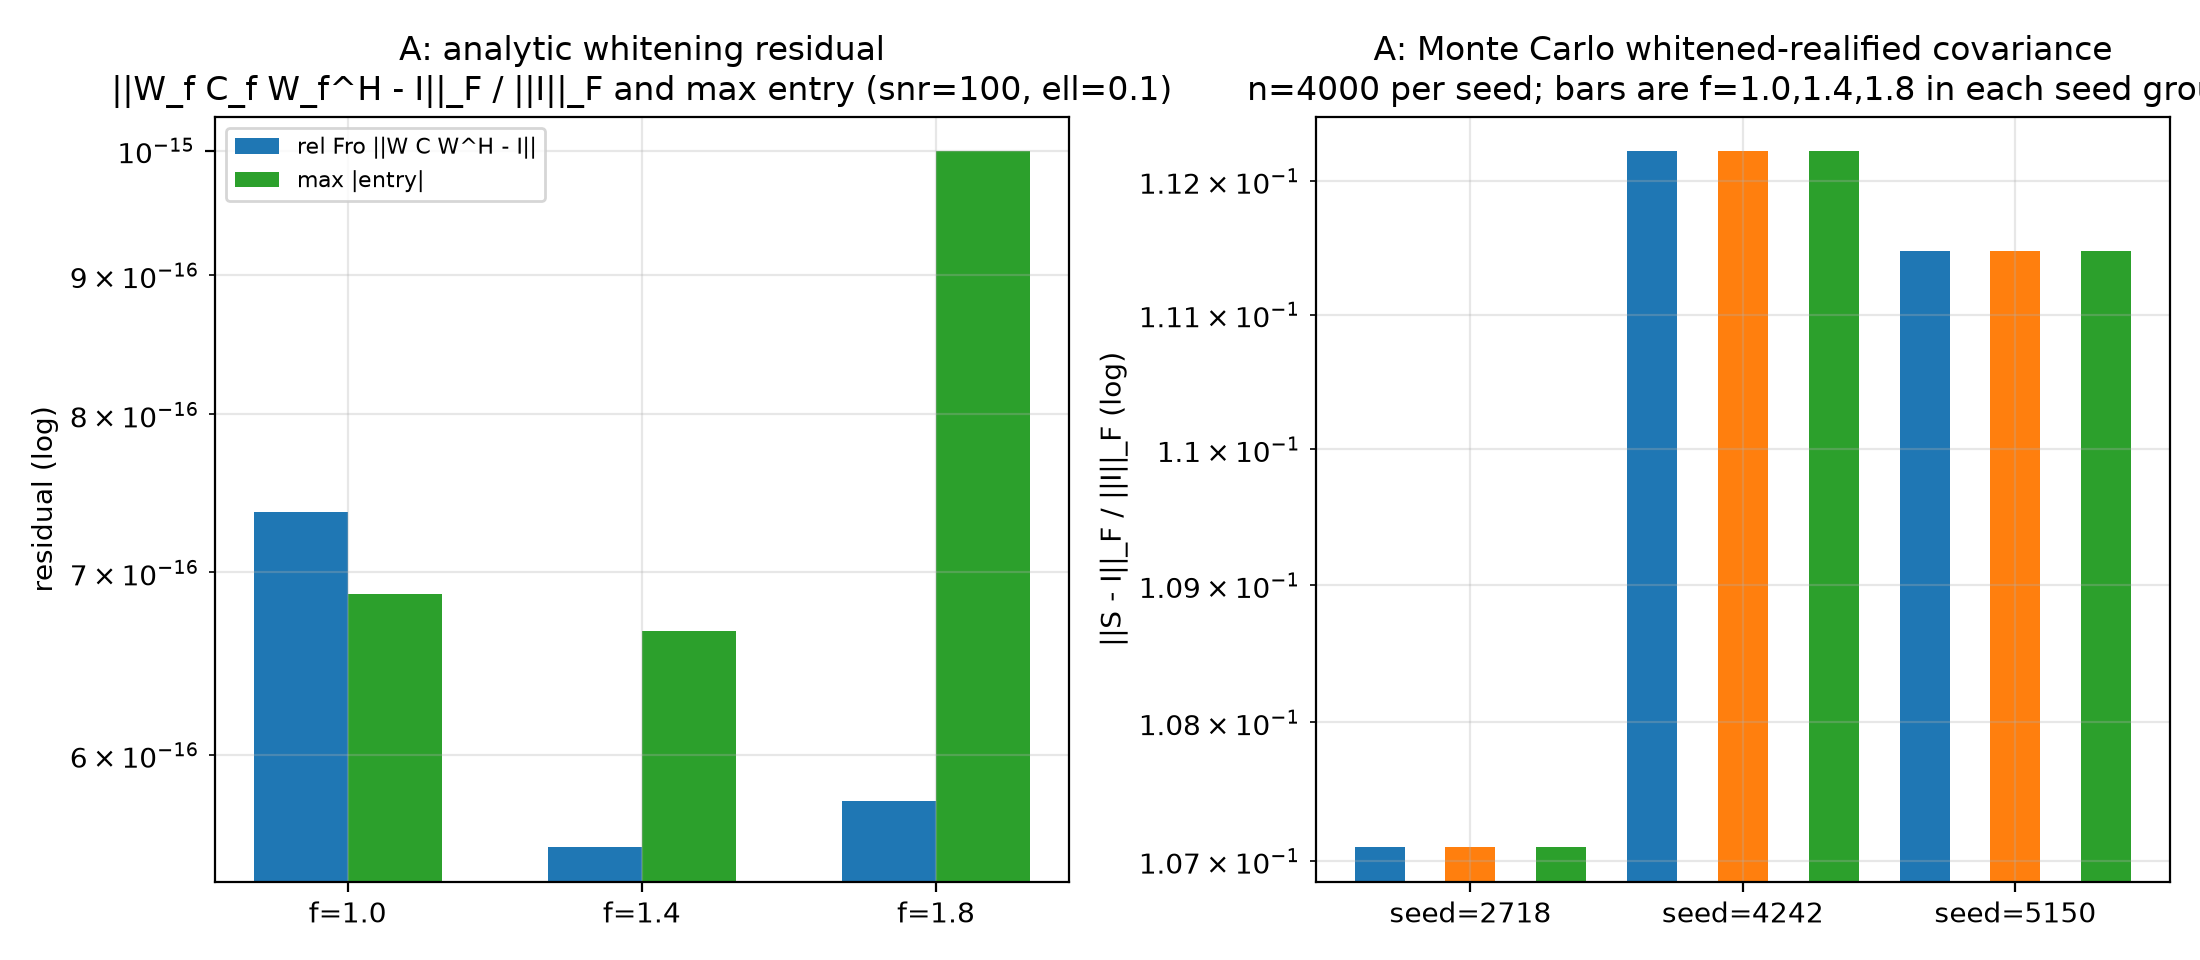
\includegraphics[width=0.86\textwidth]{../figures/family6_noise_whitening_sanity.png}
\caption{Family 6 analytic and Monte-Carlo whitening sanity (recorded).}
\label{fig:f6_sanity}
\end{figure}

\begin{figure}[htbp]
\centering
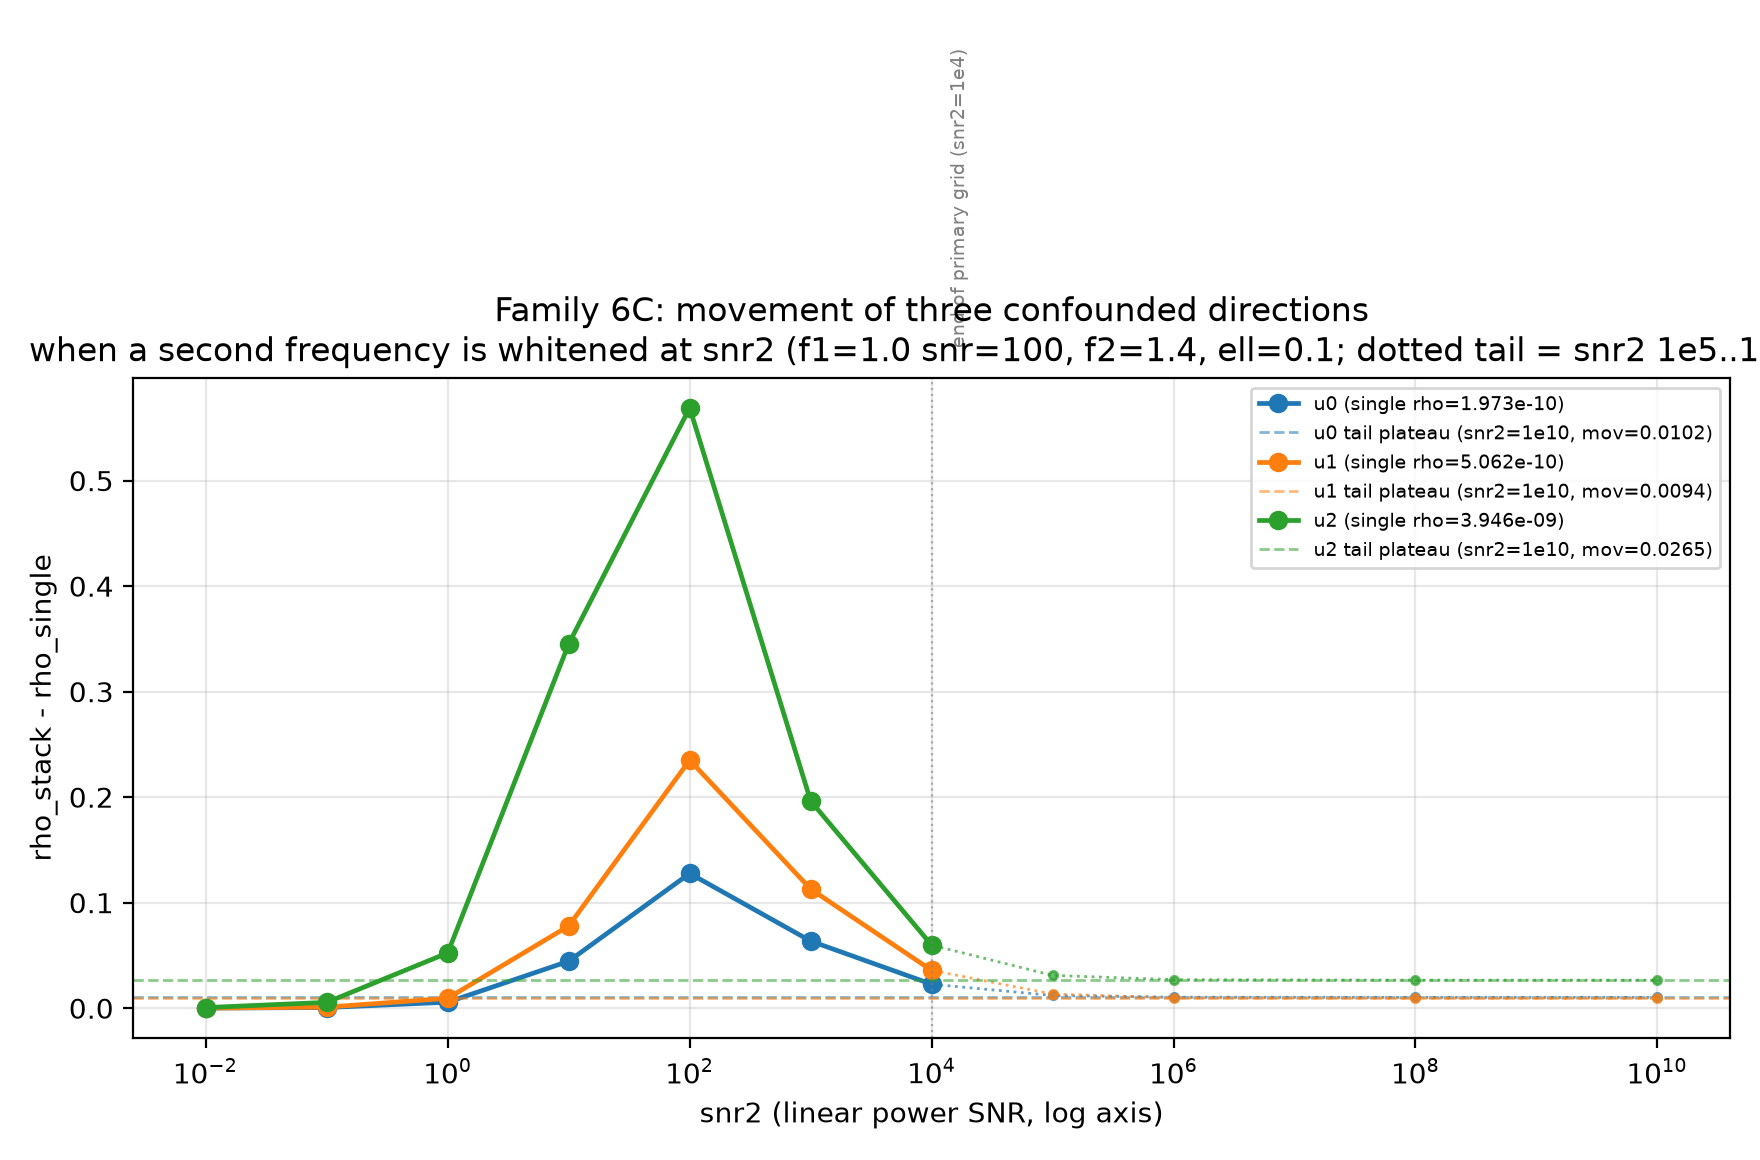
\includegraphics[width=0.86\textwidth]{../figures/family6_snr_sweep.png}
\caption{Family 6 non-monotone SNR movements with a finite high-SNR tail.}
\label{fig:f6_snr}
\end{figure}

\begin{figure}[htbp]
\centering
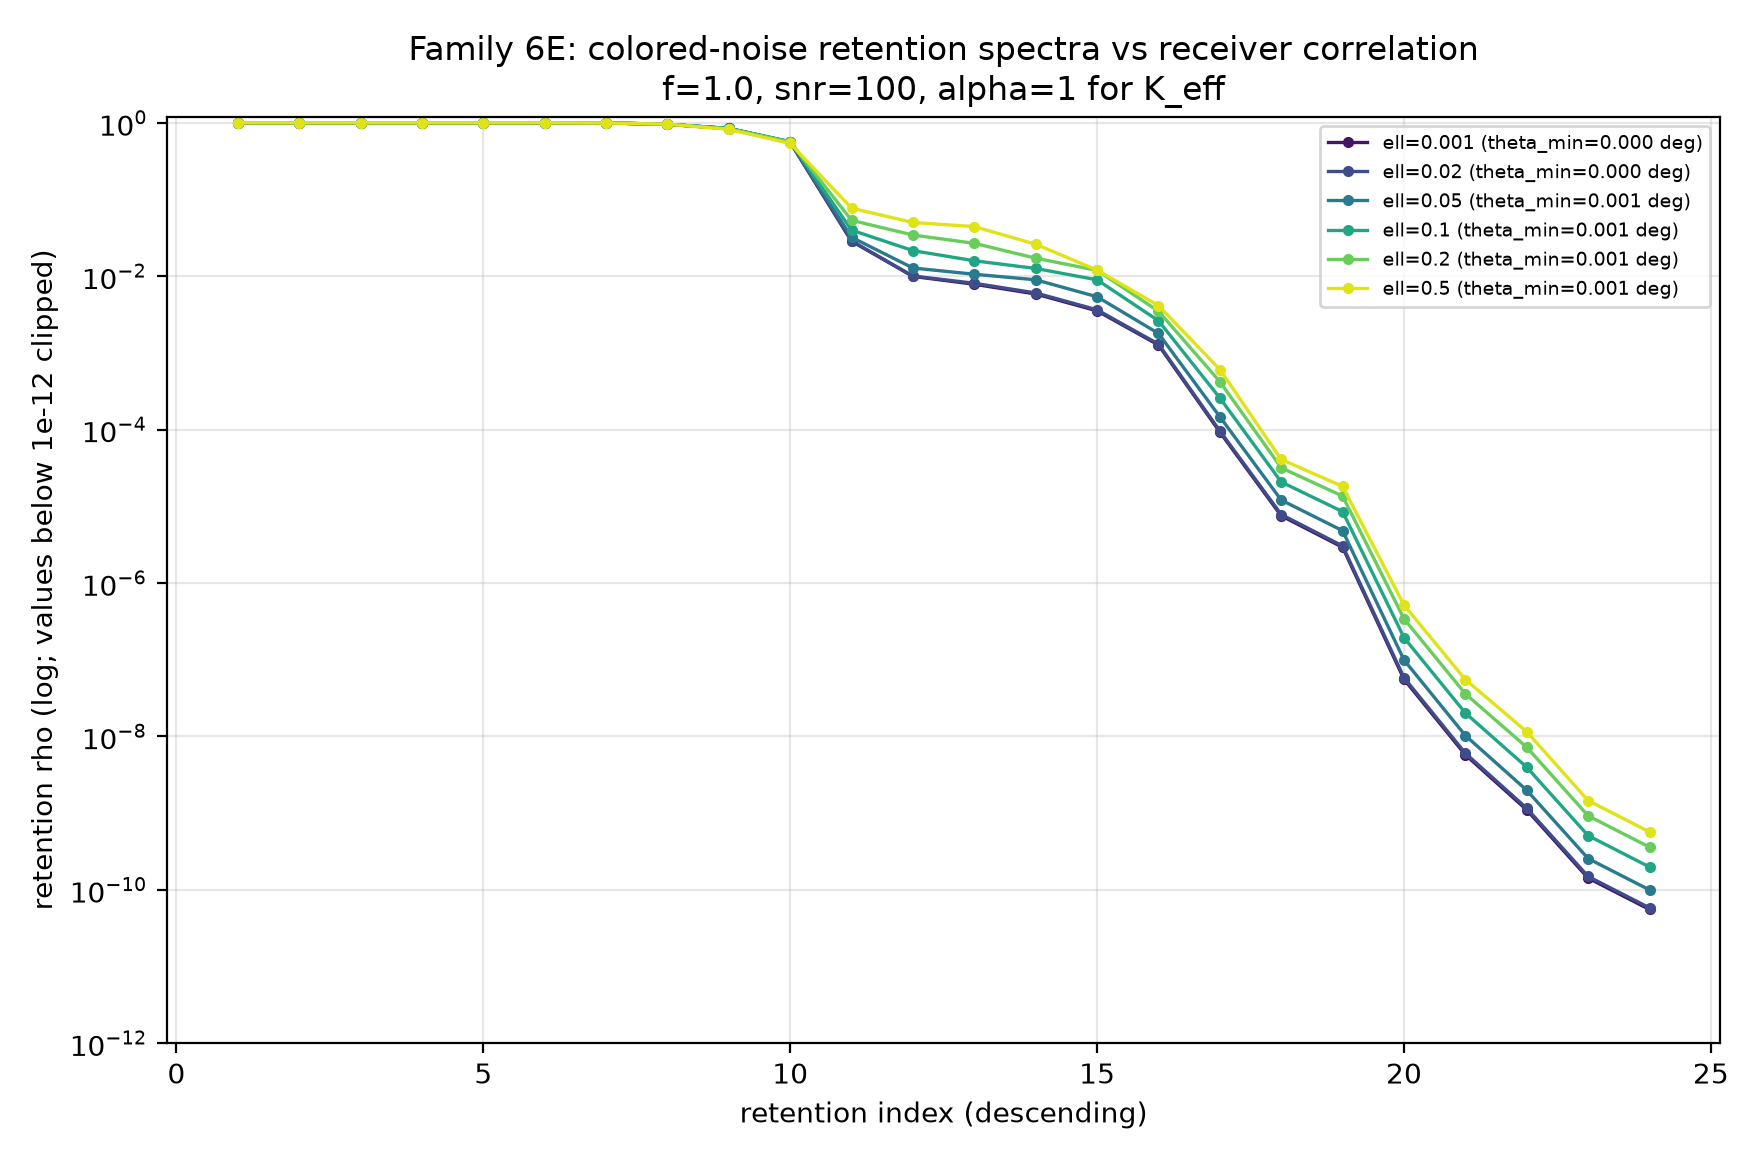
\includegraphics[width=0.86\textwidth]{../figures/family6_correlation_effect.png}
\caption{Family 6 receiver-correlation sweep (recorded, no forced pass).}
\label{fig:f6_corr}
\end{figure}

\begin{figure}[htbp]
\centering
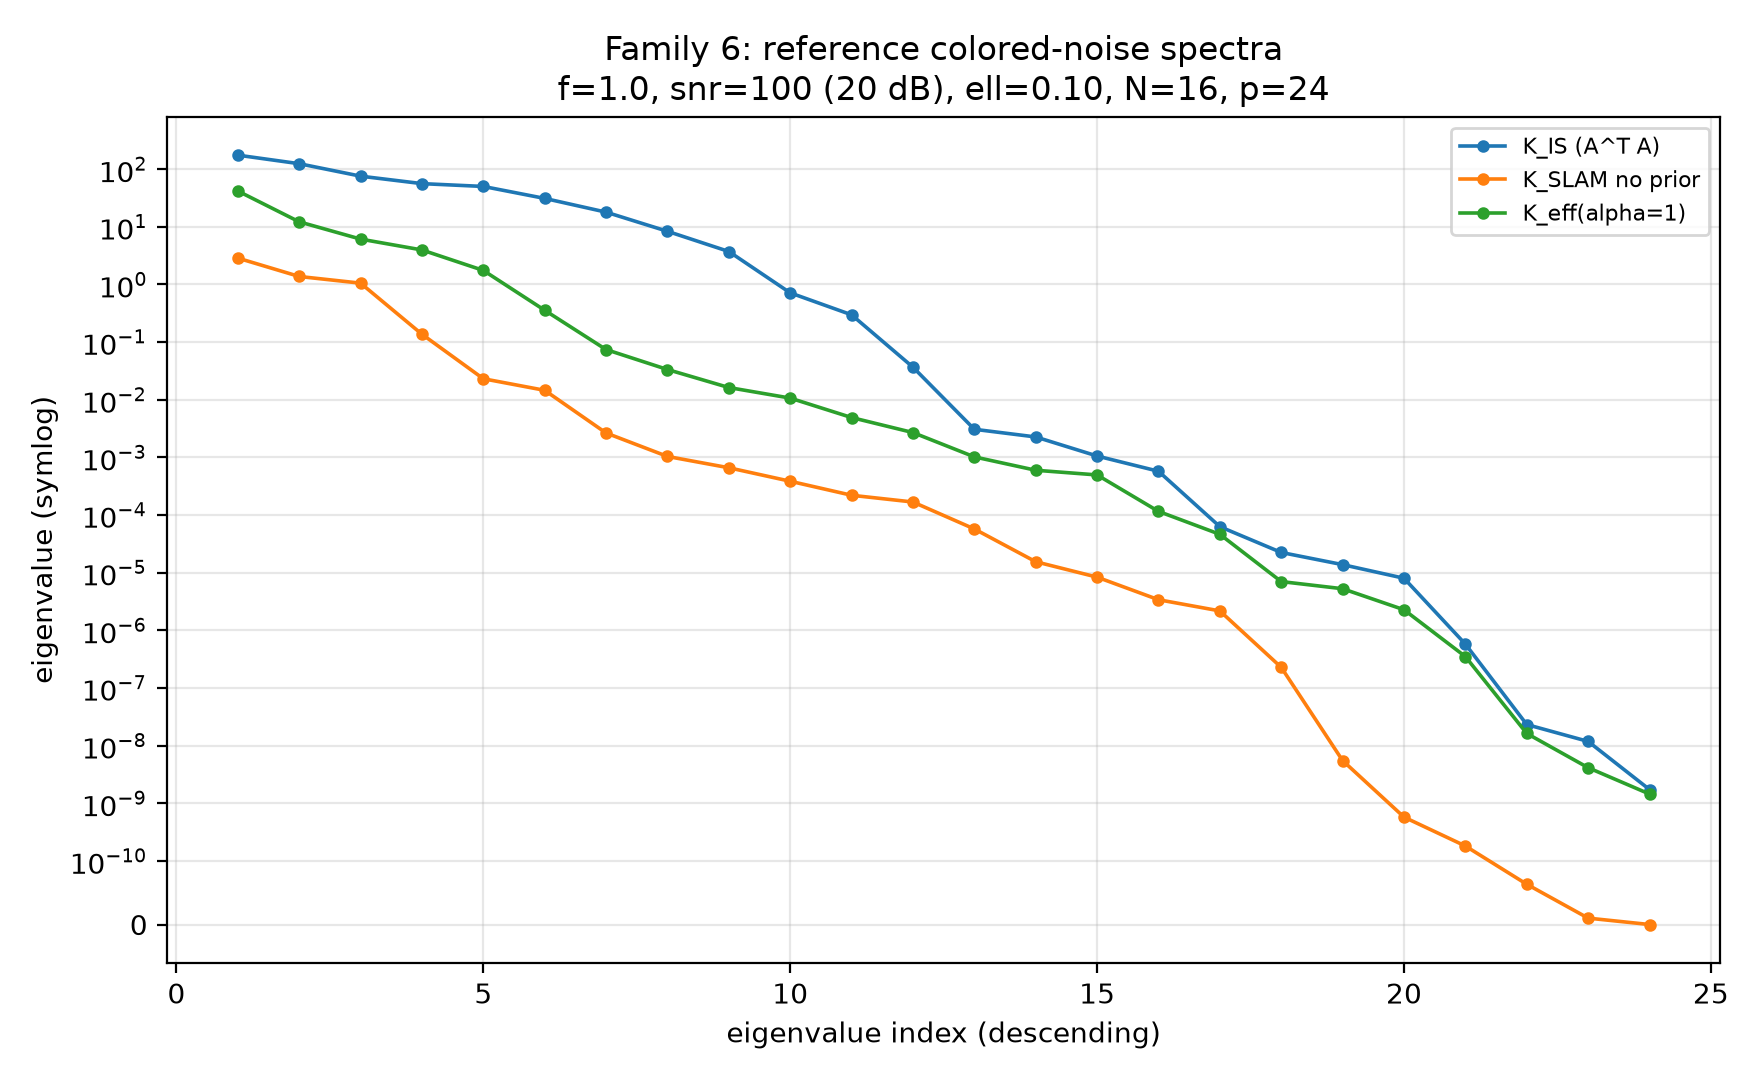
\includegraphics[width=0.86\textwidth]{../figures/family6_retention_spectra_colored.png}
\caption{Family 6 colored-noise retention spectra.}
\label{fig:f6_retention}
\end{figure}

\subsection{Trajectory control under standoff and pose-energy normalization (Family 4c)}\label{sec:family4c}

Family 4c is the Family-4 parent-audit control: curved paths are placed at a
common standoff ($R=1.6$) and each pose's realified $A$-block rows are scaled,
together with the corresponding $B$-block rows, so every pose has unit total
$A$-block Frobenius energy. Normalization is verified after the fact:
$\max|1-\|A_{\mathrm{block}}\|_F|\le2.220\times10^{-16}$ across all tested
trajectories \FDL{} (all five pass the $10^{-12}$ gate). Per-pose
normalization is a declared gain control on the linearized blocks; it does
not prescribe a physical noise covariance.

\begin{table}[htbp]
\centering
\small
\caption{Family 4c retained/confusable mass (raw and normalized;
\texttt{results/family4c\_trajectory\_control.json}).}
\label{tab:f4c}
\begin{tabular}{l l l l l}
\toprule
trajectory & retained (raw) & retained (norm.) &
confusable (raw) & confusable (norm.) \\
\midrule
straight\_same\_mid & 8.353517 & 8.269820 & 15.646483 & 15.730180 \\
arc90\_same\_standoff & 9.407162 & 9.408661 & 14.592838 & 14.591339 \\
arc180\_same\_standoff & 7.999302 & 7.997790 & 16.000698 & 16.002210 \\
arc270\_same\_standoff & 7.536362 & 7.535343 & 16.463638 & 16.464657 \\
circle360\_same\_standoff & 7.703633 & 7.701223 & 16.296367 & 16.298777 \\
\bottomrule
\end{tabular}
\end{table}

The raw and normalized orderings do not flip \OBS{}: retained mass descends as
arc90 $>$ straight $>$ arc180 $>$ circle360 $>$ arc270 in both columns, and
confusable mass ascends in the same order. The four-core hypothesis
(circle360 $>$ arc180 $>$ arc90 $>$ straight) therefore remains false under
the normalized control: \texttt{hypothesis\_holds\_for\_four\_core=false},
recorded without a forced pass. This preserves the Family 4 trajectory
counterexample \CTX{} under a cleaner geometry control; arc270 is the lowest
retained-mass trajectory in this five-path set. No universal trajectory
ordering is asserted: equal standoff fixes curved-path range but still changes
continuous design length and sampled polyline length with angular coverage,
and the straight path still varies standoff \OBS{}.

\begin{figure}[htbp]
\centering
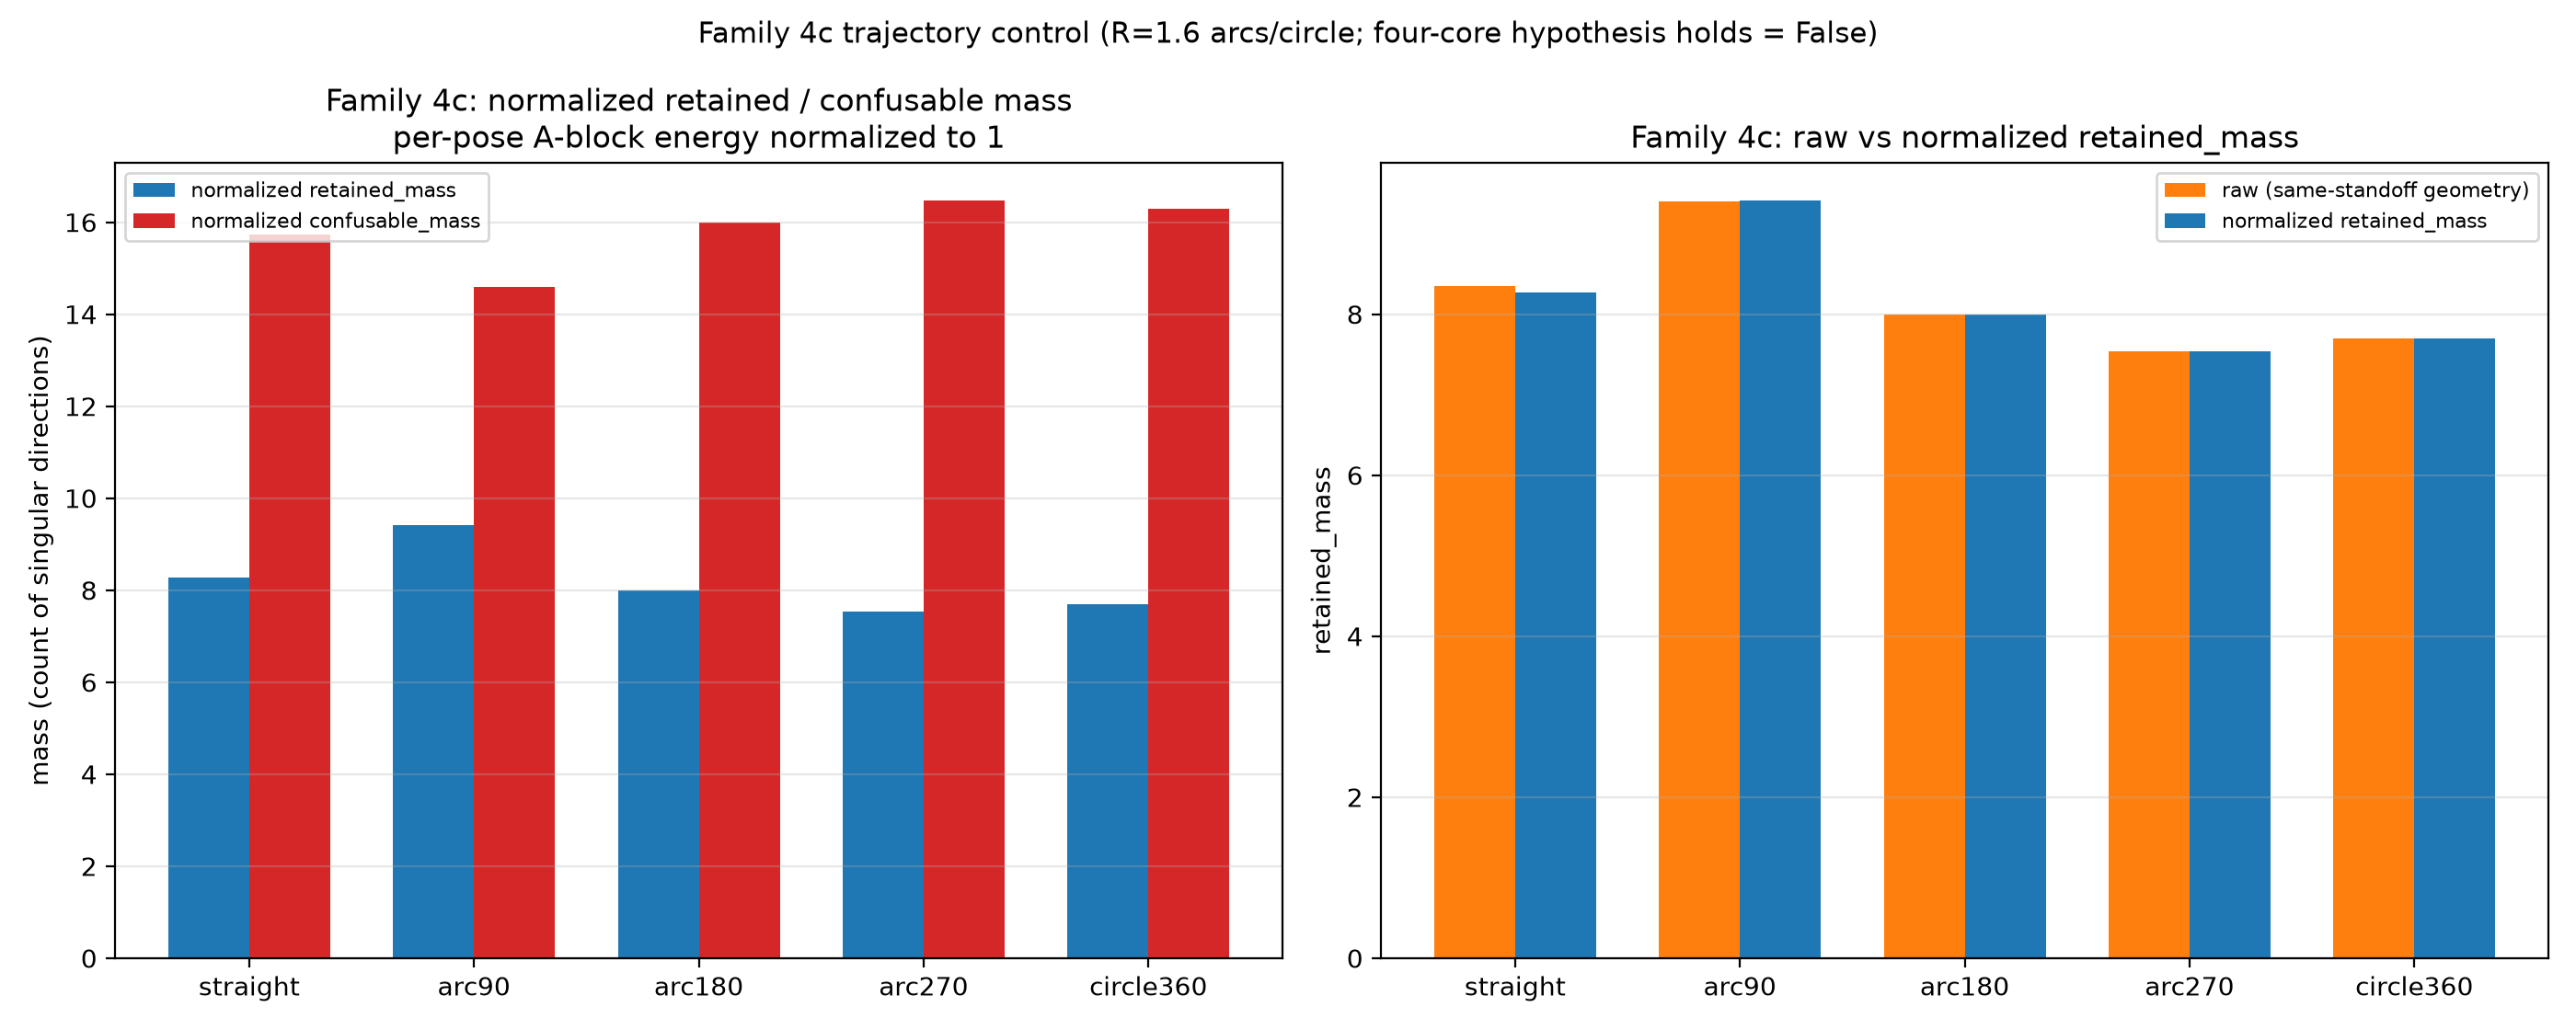
\includegraphics[width=0.86\textwidth]{../figures/family4c_trajectory_control.png}
\caption{Family 4c same-standoff raw and normalized trajectory control.}
\label{fig:f4c}
\end{figure}

\subsection{Resolution, rank events, and stable-transversality diagnostics (Family 7)}\label{sec:family7}

Family 7 is a new finite-grid diagnostic family: for every resolution $N$ the
same continuous two-blob scene is sampled on that grid and the smooth p=24
basis is rebuilt, and separate frequency and contrast sweeps are recorded at
N=16. These are diagnostics on the executed grids, explicitly not continuum
or transversality proofs \OBS{}.

\begin{table}[htbp]
\centering
\small
\caption{Family 7 key numbers by resolution
(\texttt{results/family7\_refinement\_rank.json}).}
\label{tab:f7}
\begin{tabular}{p{0.38\textwidth} p{0.54\textwidth}}
\toprule
quantity & value \\
\midrule
ranks at N=16/24/32/40/48 & $r_A=24$, $r_B=18$, $r_{AB}=42$, $r_{K}=24$;
rank identity true at every computed $N$ \\
$\theta_{\min}$ (deg), N=16 to 48 &
$4.253070\times10^{-4}$ to $4.188332\times10^{-4}$ (monotone decreasing,
span $6.474\times10^{-6}$ deg) \\
near-confounded directions (cos$^2>1-10^{-8}$) &
$[4,4,4,4,4]$; constant over the tested grid \\
frequency sweep (21 points, f=0.6..2.6) &
rank events 0; 21 literal near-crossing flags, all on the lowest
numerical near-null $K_{\mathrm{eff}}$ pairs \\
$s=0$ Born gates &
B/A Fro ratio 0.0; rel.\ Fro $K_{\mathrm{SLAM}}-K_{\mathrm{IS}}$ 0.0
(both pass $<10^{-12}$) \\
Born/full rel.\ Fro discrepancy &
$1.894\times10^{-3}$ at $s=0.01$ growing to $0.1975$ at $s=1$ \\
contrast rank transition & expected $s=0\to0.01$ exit
($r_B:0\to18$, $r_{AB}:24\to42$), recorded as an observed machine-rank event \\
\bottomrule
\end{tabular}
\end{table}

Across N=16..48 the machine ranks remain constant and the rank identity passes
for every computed row \FDL{}. The minimum principal angle
$\theta_{\min}$ decreases monotonically on the tested grid
($4.253070\times10^{-4}$ to $4.188332\times10^{-4}$ deg), and the number of
near-confounded directions is constant at 4 \OBS{}. In the frequency sweep no
rank event occurs, but every one of the 21 sweep points satisfies the literal
smallest-gap near-crossing inequality on one of the lowest ascending pairs
([0,1] or [1,2]); those flags sit in the repeated numerical near-null tail of
$K_{\mathrm{eff}}$ and are recorded as the literal criterion, not as certified
eigenvalue crossings or transversality failures. The $s=0$ Born gates pass
exactly \FDL{} ($B=0$ and $K_{\mathrm{SLAM}}=K_{\mathrm{IS}}$ to the declared
$10^{-12}$ relative gate), while the Born/full-wave discrepancy grows from
$1.894\times10^{-3}$ at $s=0.01$ to $0.1975$ at $s=1$ \OBS{}. No forced pass
is applied anywhere in Family 7.

\begin{figure}[htbp]
\centering
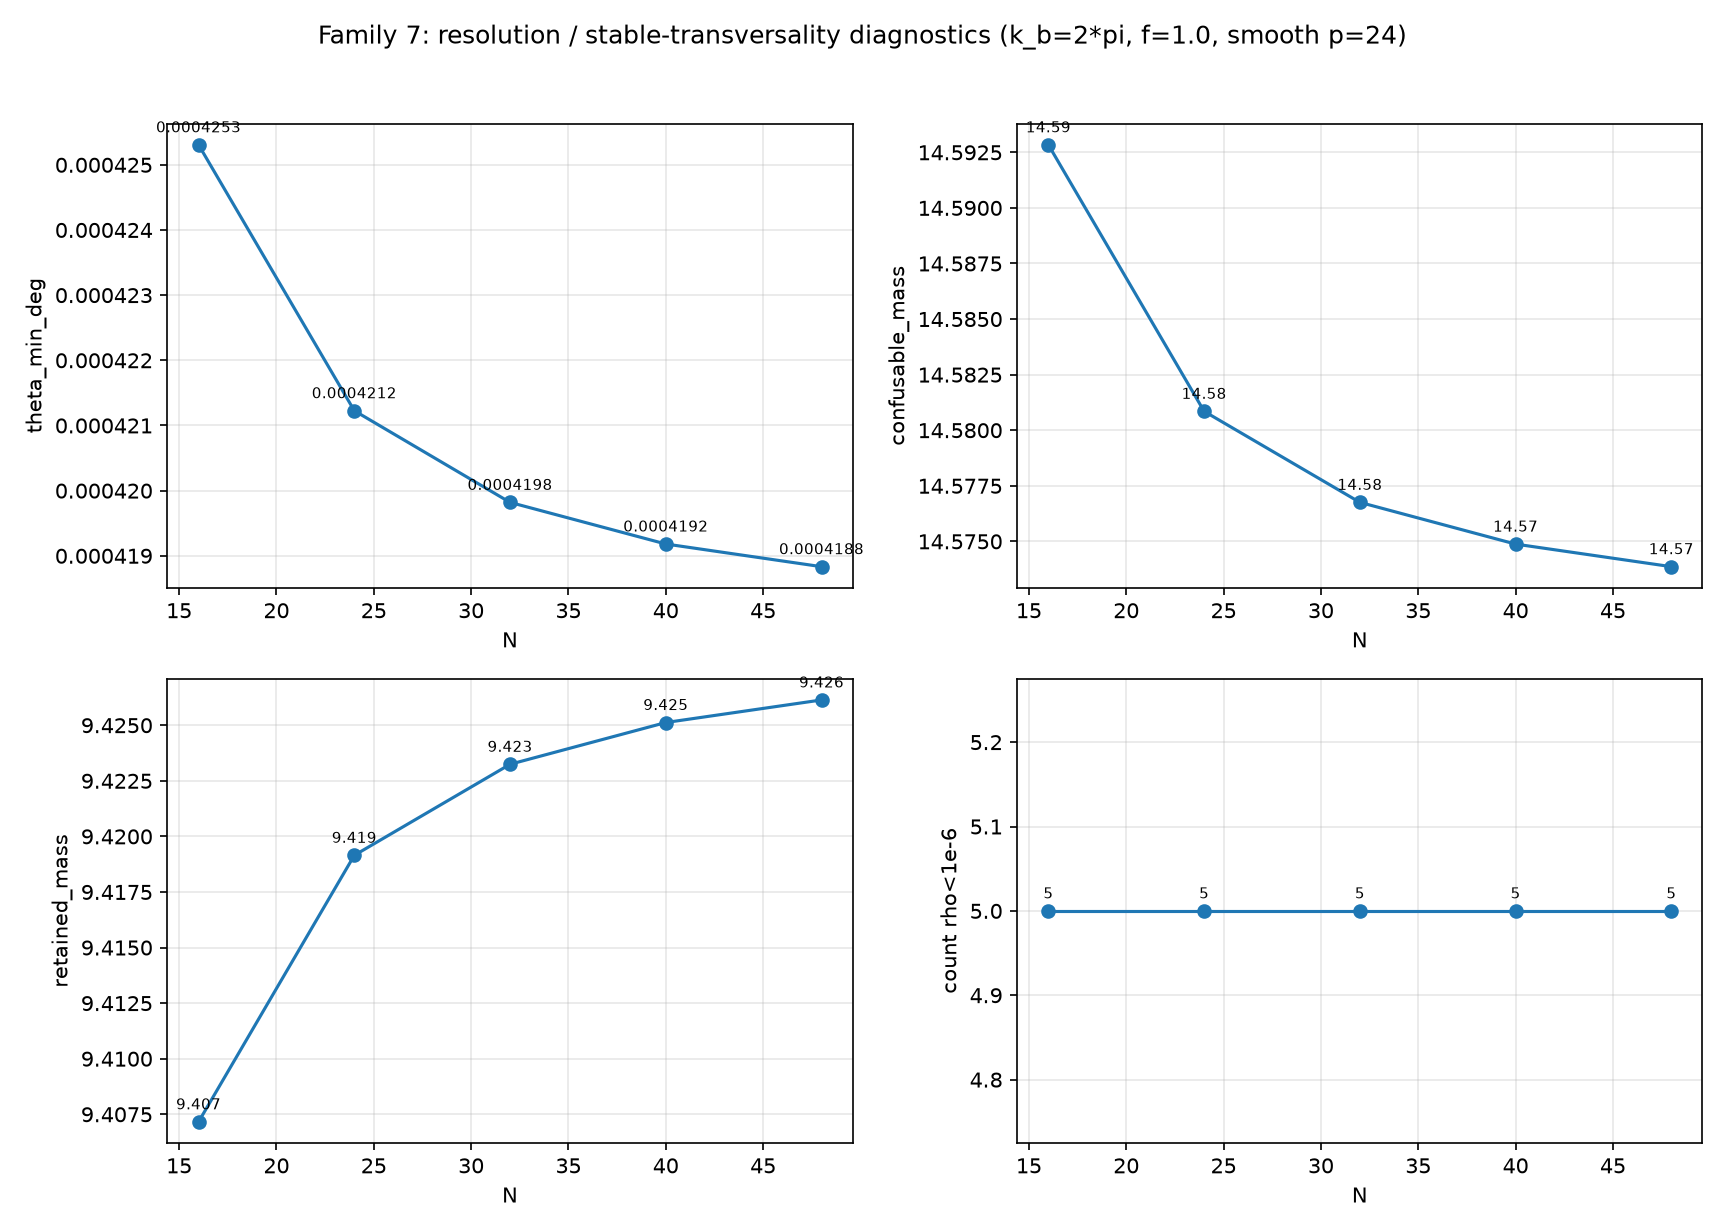
\includegraphics[width=0.86\textwidth]{../figures/family7_resolution_convergence.png}
\caption{Family 7 resolution convergence of $\theta_{\min}$ and spectral masses.}
\label{fig:f7_resolution}
\end{figure}

\begin{figure}[htbp]
\centering
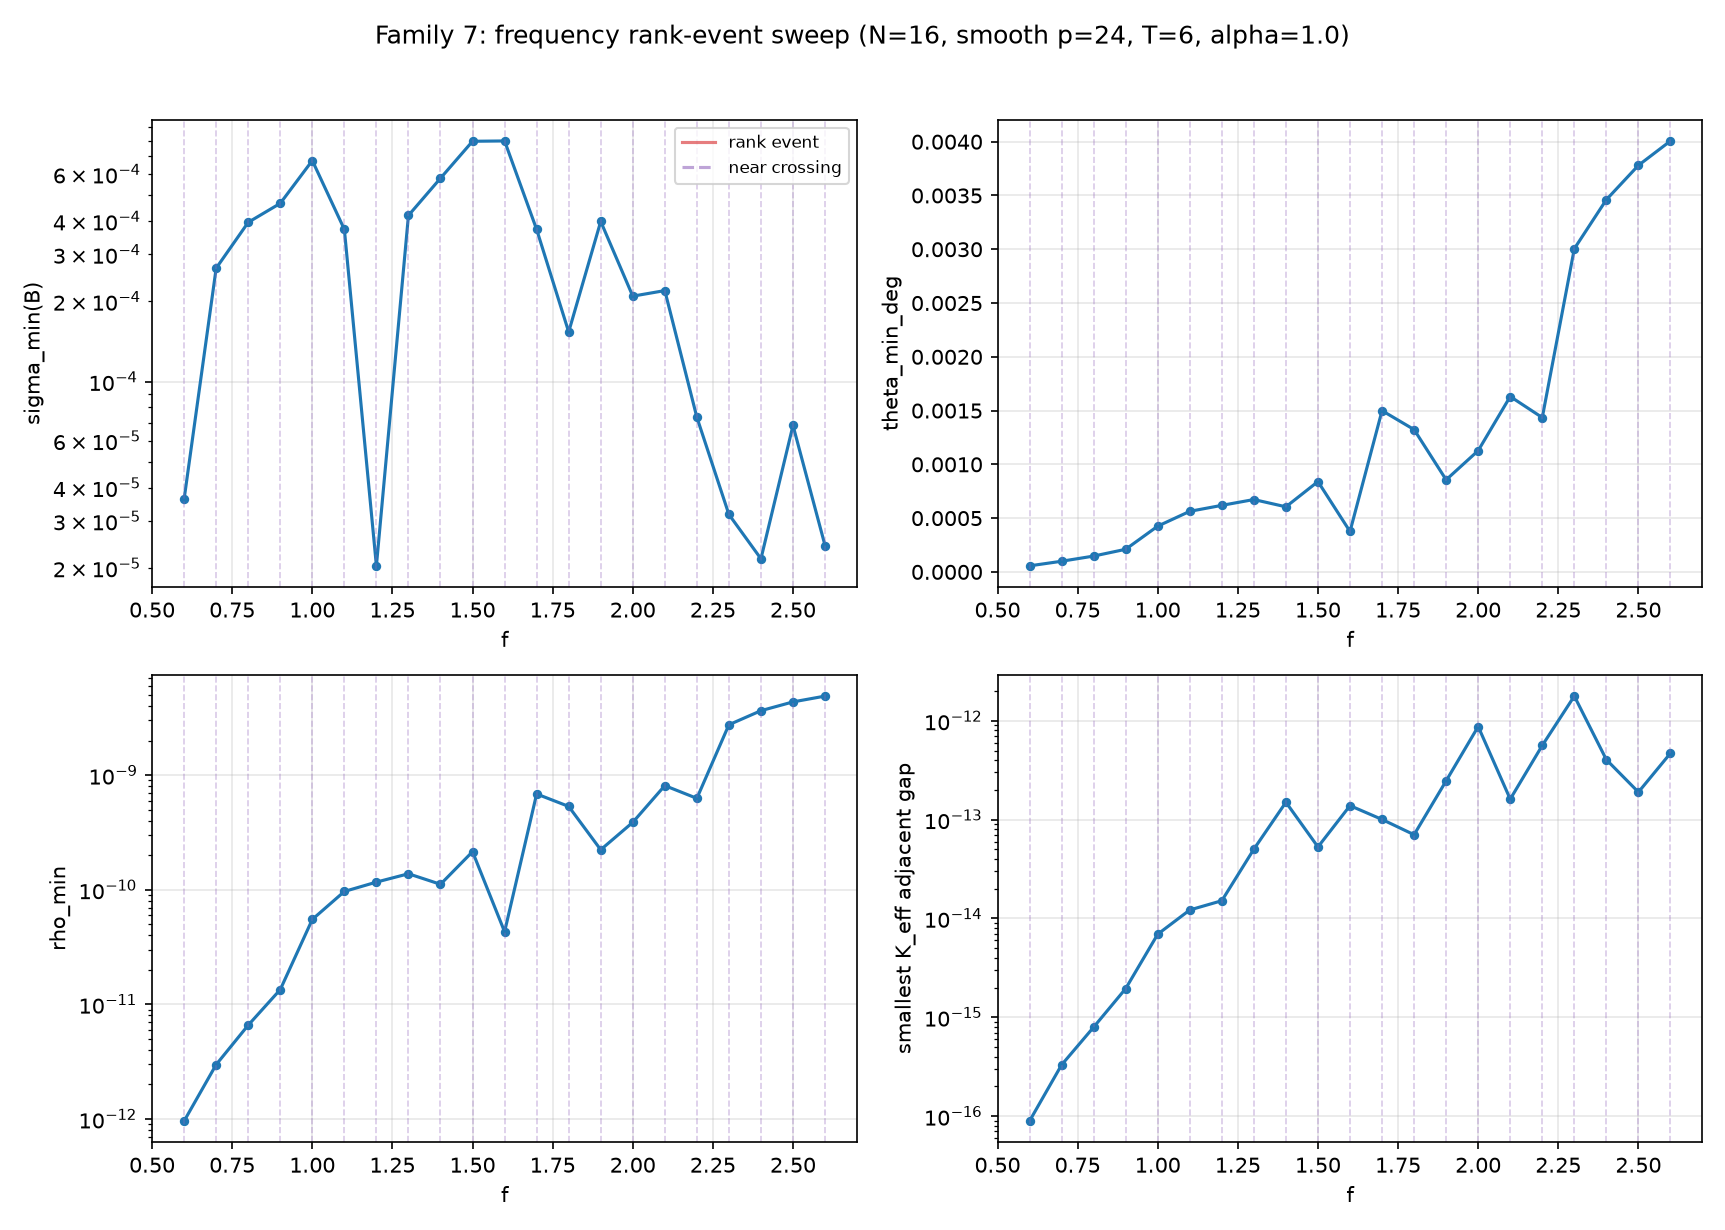
\includegraphics[width=0.86\textwidth]{../figures/family7_frequency_rank_sweep.png}
\caption{Family 7 frequency rank-event and near-crossing sweep.}
\label{fig:f7_frequency}
\end{figure}

\begin{figure}[htbp]
\centering
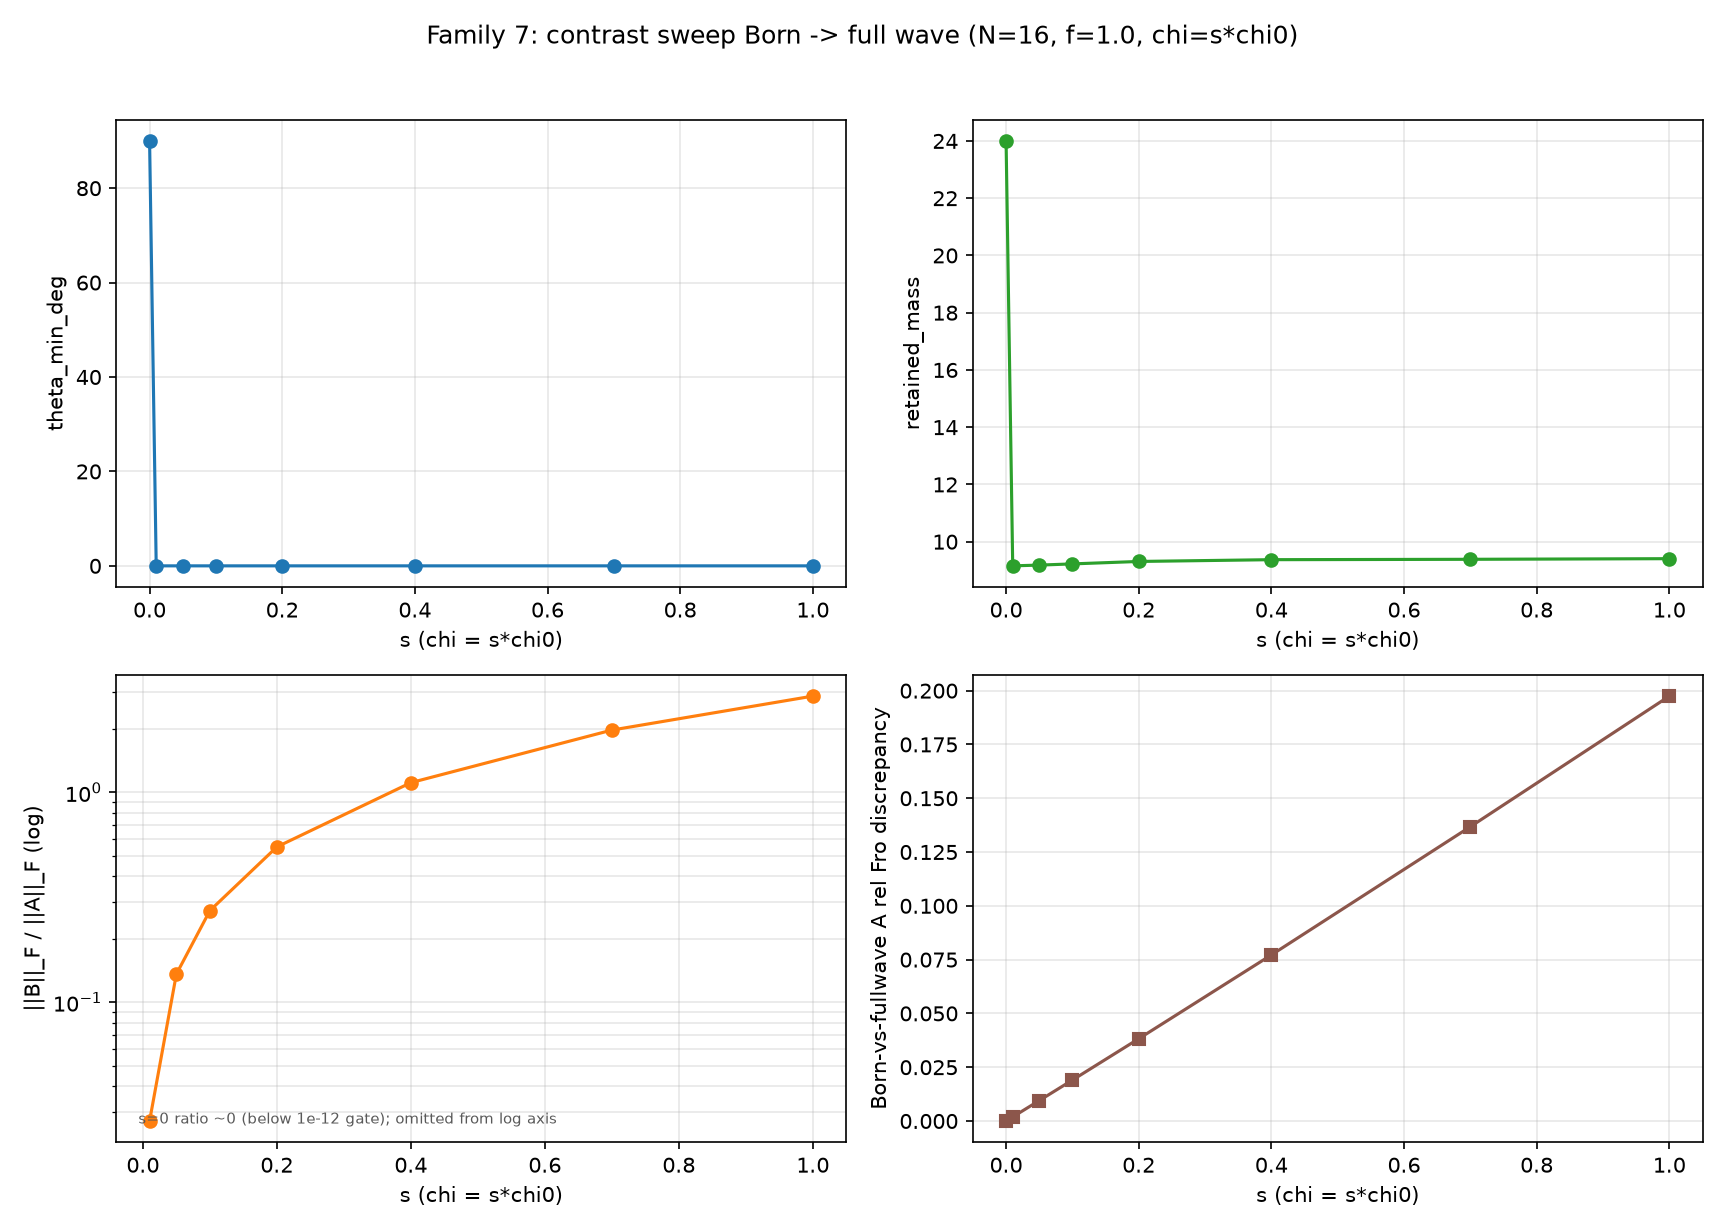
\includegraphics[width=0.86\textwidth]{../figures/family7_contrast_sweep.png}
\caption{Family 7 Born-to-full-wave contrast sweep.}
\label{fig:f7_contrast}
\end{figure}

\subsection{Current-space $G_S$/SOM vs map-tangent $A/K_{\mathrm{eff}}$ distinction (Family 8)}\label{sec:family8}

Family 8 makes the current-space sensing map $G_S$ (stacked over poses) and
the map-tangent Jacobian $A_c$/pixel kernel $K_{\mathrm{eff}}$ explicit in the
same $N^2$ pixel space, at N=16, T=6, f=1.0, with $\alpha=1.0$.

\begin{table}[htbp]
\centering
\small
\caption{Family 8 key numbers
(\texttt{results/family8\_som\_distinction.json}).}
\label{tab:f8}
\begin{tabular}{p{0.38\textwidth} p{0.54\textwidth}}
\toprule
quantity & value \\
\midrule
full-wave composition stack rel.\ Fro &
0 (identical float path; per-pose 0) \\
Born composition stack rel.\ Fro & $7.05442\times10^{-17}$ \\
Range$(A_c)\subseteq$Range$(G_S)$ &
projector difference $3.5260\times10^{-15}$; containment residual
$2.3354\times10^{-15}$; ranks 24 $\le$ 24 \\
literal arccos angle (U subspaces) &
$2.1073\times10^{-8}$ rad, the $\sqrt{2\epsilon}$ roundoff floor;
literal rad gate false \\
right-subspace principal angles $V_{GS}$ vs $V_A$ &
count $<10^{-8}$ deg: 0/24; median $29.70670$ deg; max $89.79380$ deg; \\
 & min $0.46609$ deg; row-proj diff 0.999994 \\
$K_{\mathrm{eff}}$ confounded-vector overlaps &
max squared overlaps with $V_{GS}$: $3.2680\times10^{-3}$; \\
 & with $V_A$: $5.7556\times10^{-8}$ \\
mode counts at rel.\ thresholds $10^{-6}$/$10^{-3}$ &
$\sigma(G_S)$ [13, 8]; $\sigma(A_c)$ [23, 12]; \\
 & $\sigma(A_R)$ [46, 23]; eig$(K_{\mathrm{IS}})$ [23, 12] \\
\bottomrule
\end{tabular}
\end{table}

The full-wave composition identity is bit-identical (stack relative Frobenius
0), and the Born composition identity holds to $7.054\times10^{-17}$
\FDL{}. Range containment of $A_c$ in $G_S$ holds machine-exactly on the
tested full-rank data space (projector difference $3.526\times10^{-15}$ and
containment residual $2.335\times10^{-15}$) \FDL{}; the recorded arccos angle
sits at the roundoff floor for identical full-rank subspaces, so the direct
O($\epsilon$) projector/residual checks are the meaningful gates. By contrast,
the right singular pixel-mode subspaces $V_{GS}$ and $V_A$ are strongly
distinct \OBS{}: zero of 24 principal angles fall below $10^{-8}$ deg, the
median is $29.70670$ deg, the maximum is $89.79380$ deg, and the row-space
projector difference is 0.999994 (nearly orthogonal). The three most
confounded $K_{\mathrm{eff}}$ directions are nearly orthogonal to both mode
sets on the tested scenario: their maximum squared overlaps are about
$3\times10^{-3}$ with $V_{GS}$ and only about $6\times10^{-8}$ with $V_A$.
Mode counts also differ once the different threshold scales are recorded
side by side (SOM count vs map-information count), and no SOM quality claim
is made.

\begin{figure}[htbp]
\centering
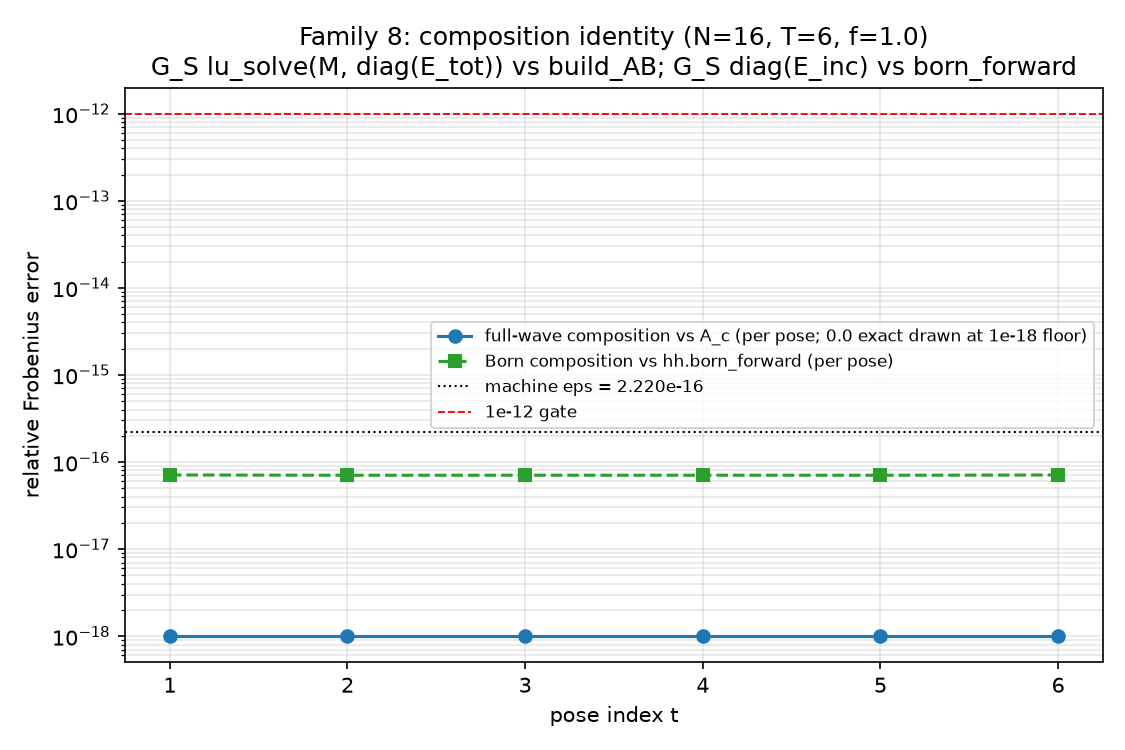
\includegraphics[width=0.86\textwidth]{../figures/family8_composition_identity.png}
\caption{Family 8 per-pose full-wave and Born composition identities.}
\label{fig:f8_composition}
\end{figure}

\begin{figure}[htbp]
\centering
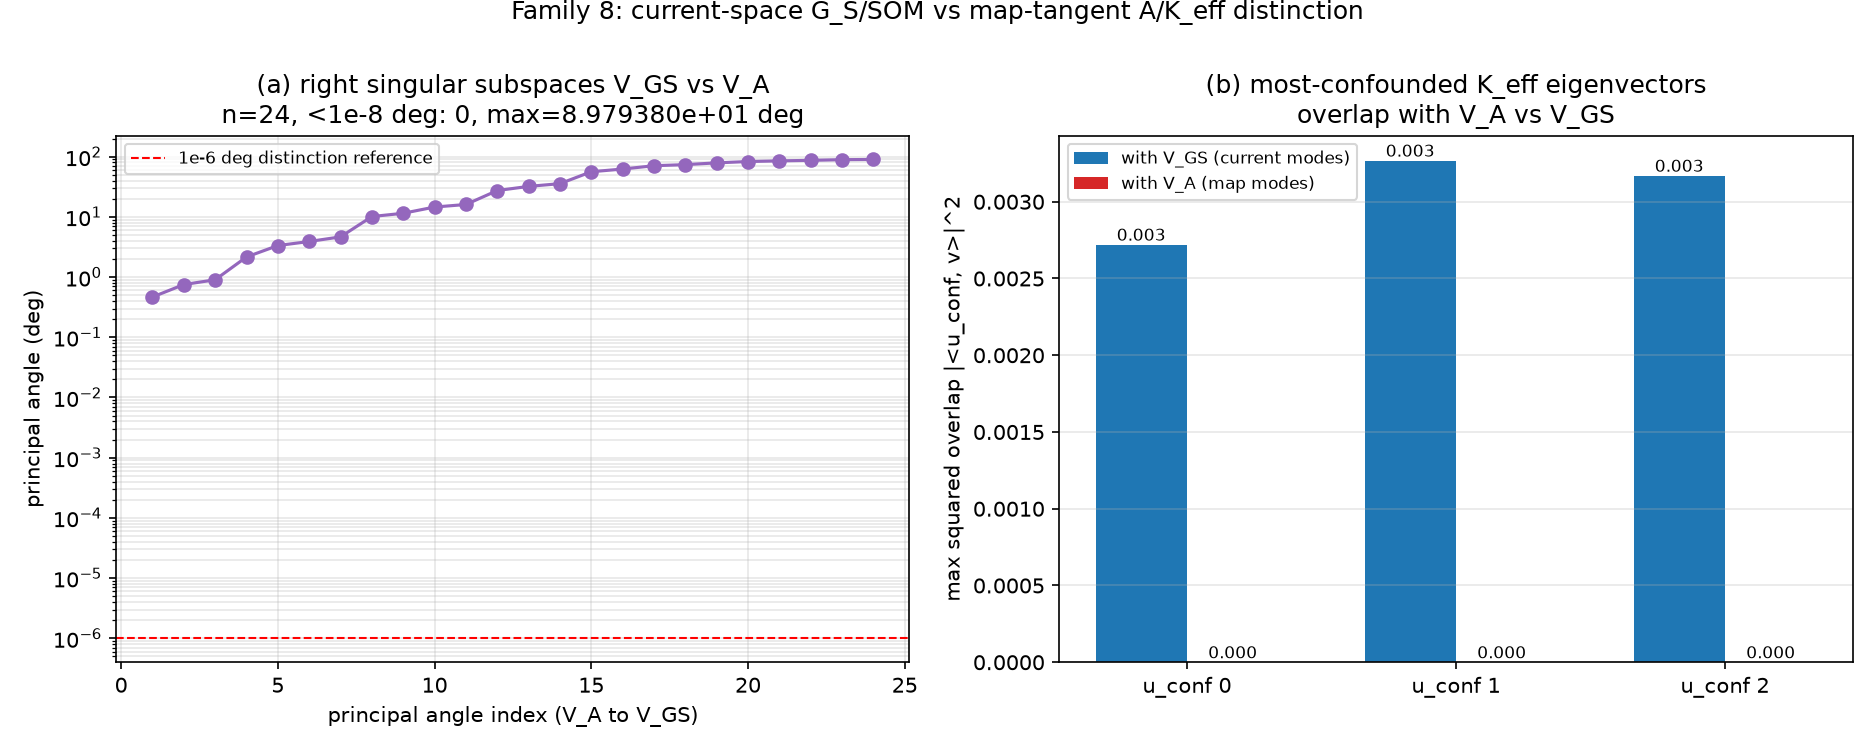
\includegraphics[width=0.86\textwidth]{../figures/family8_mode_distinction.png}
\caption{Family 8 principal-angle and overlap distinction between
$V_{GS}$/SOM and $V_A$/$K_{\mathrm{eff}}$ mode families.}
\label{fig:f8_modes}
\end{figure}

\subsection{Seed replications and component ablations (Family 9)}\label{sec:family9}

Family 9 reruns the deterministic Family 2 (c1--c3) and Family 4 check-C
claims over seven scenes (five 8-blob seeds 1001--1005 rescaled to the
two-blob norm, the standard two-blob scene, and a ring scene) and records
descriptive component ablations.

\begin{table}[htbp]
\centering
\small
\caption{Family 9 replication and ablation key numbers
(\texttt{results/family9\_replications\_ablation.json}).}
\label{tab:f9}
\begin{tabular}{p{0.38\textwidth} p{0.54\textwidth}}
\toprule
quantity & value \\
\midrule
rank identity over 7 scenes & 6/7; ring residual 1 (machine-rank boundary) \\
no-prior retention identity & 7/7 (max diff $2.817\times10^{-15}$;
typical $\sim10^{-15}$) \\
kernel identity & F2 subspace gate 7/7; identity support 6/7;
nullity match 6/7 (ring mismatch) \\
frequency diversity & 7/7; 3/3 directions moved above $10^{-4}$ on every scene \\
pose-DOF retained mass & known 24.000; x-only 18.020; y-only 18.029;
$\theta$-only 21.362; \\
 & xy 12.573; full 9.407 \\
receiver-count retained mass ($n_{\mathrm{rx}}$=1/2/4/8) &
0 / 6.000 / 9.407 / 9.399 (mixed-$r_A$ rows; not a pure effect) \\
pose-count retained mass (T=3/6/12) &
15.000 / 9.407 / 6.579 (monotone on this grid) \\
basis retained mass (p=12/24/36) &
0.157 / 9.407 / 18.750 (fixed $B$ adds $A$ directions) \\
\bottomrule
\end{tabular}
\end{table}

The replication record is \FDL{} on the executed scenes where the gates pass,
with one preserved boundary event: the ring scene's smallest
$K_{\mathrm{SLAM}}$ eigenvalue falls below the family-2 eig rank tolerance
while $C=(I-ZZ^T)A_s$ remains full rank at its own SVD tolerance, so the
literal machine-rank identity records residual 1 and nullity mismatch.
That ring row is a recorded machine-rank boundary, not evidence against the
exact algebraic identity \OBS{}. Retention and frequency diversity pass on
all seven scenes. The ablations are descriptive, with no forced pass:
$\theta$-only nuisance destroys less retained mass than the translational
DOFs, receiver-count rows mix changing $r_A$ with receiver count and are not
interpreted as a pure effect, pose-count retention declines monotonically on
the tested T grid as more nuisance columns are added, and basis-p retention
grows with $r_A$ for a fixed $B$. No universal claim is drawn from these
single-geometry trends.

\begin{figure}[htbp]
\centering
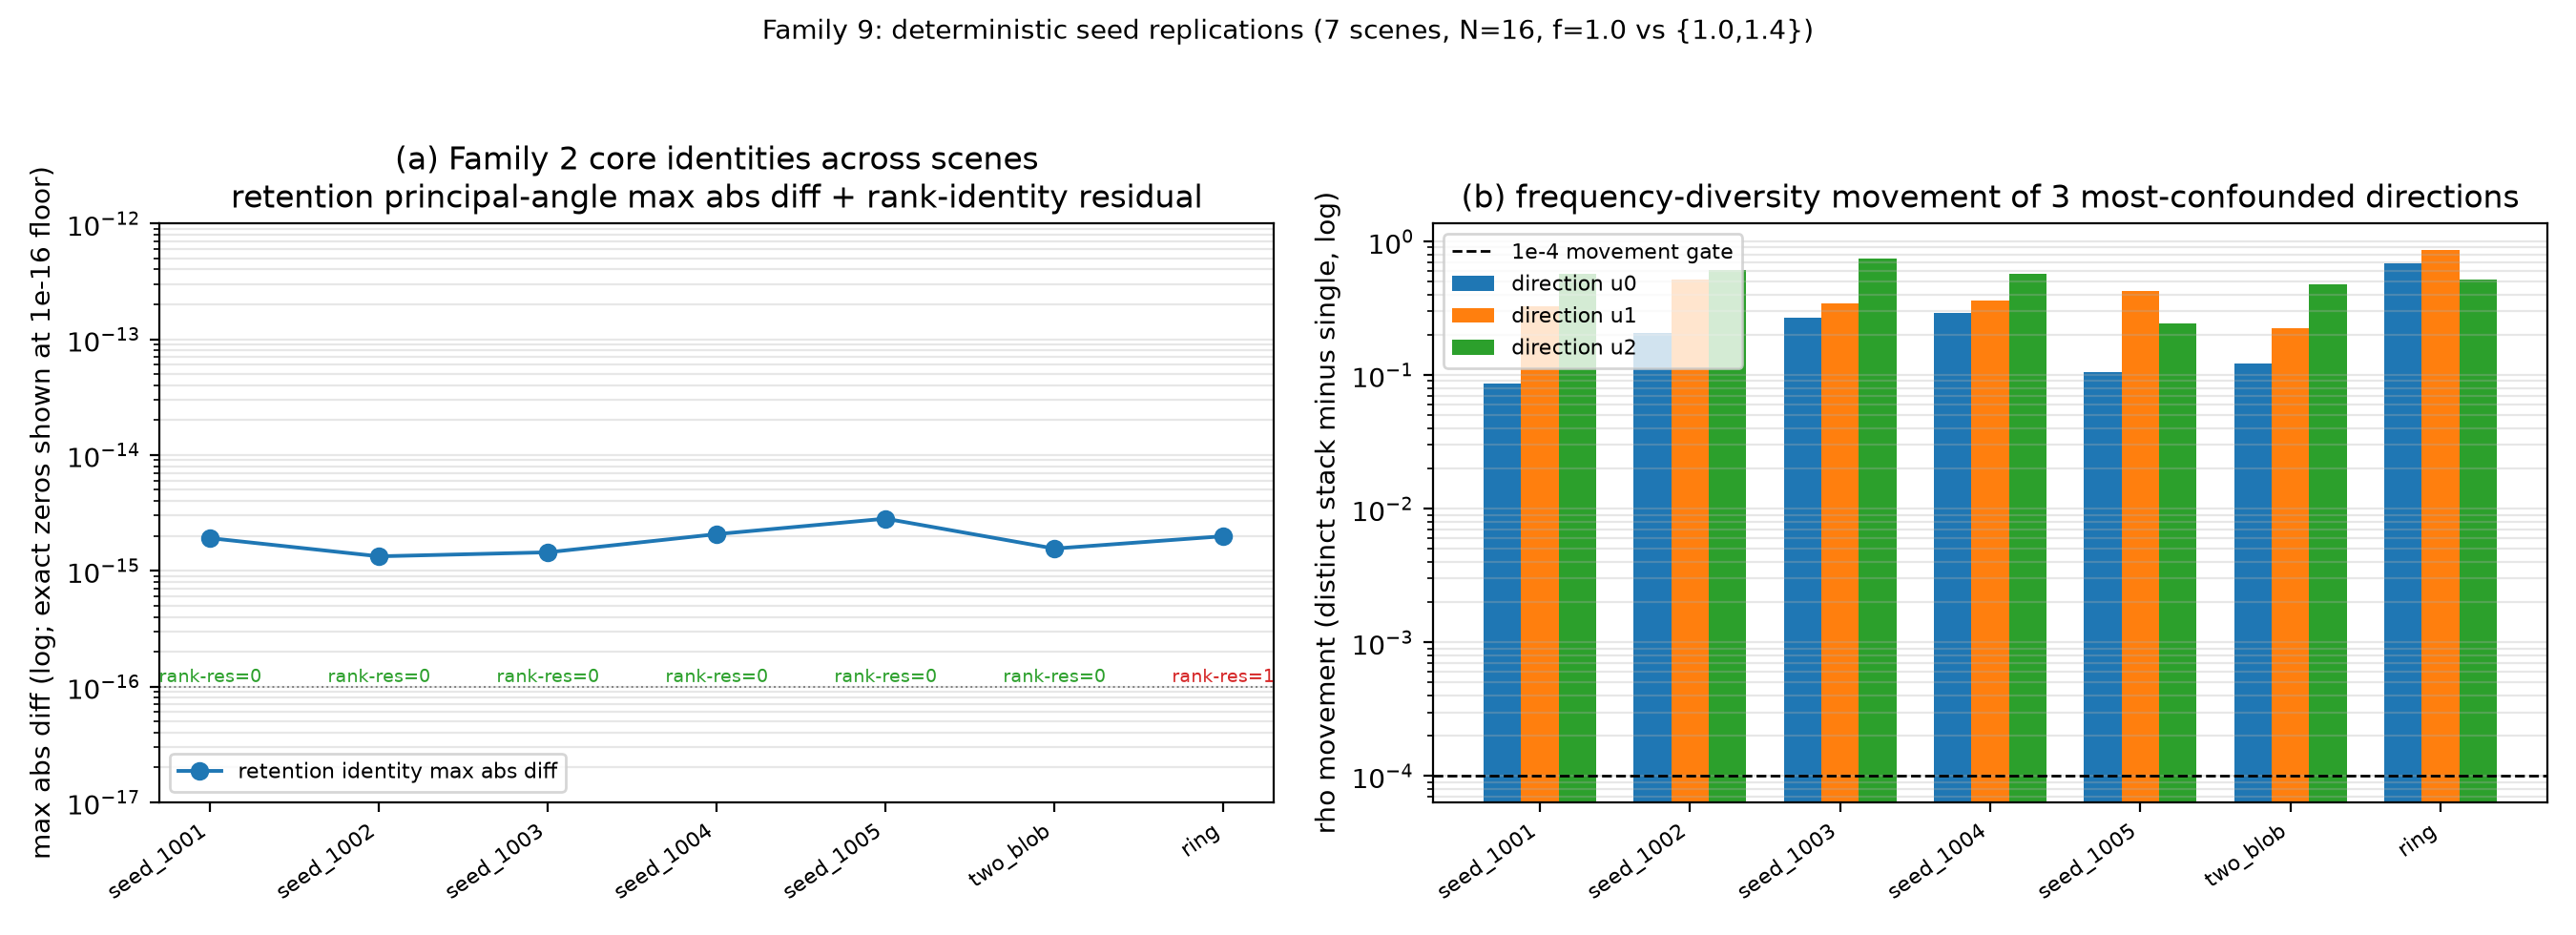
\includegraphics[width=0.86\textwidth]{../figures/family9_seed_replications.png}
\caption{Family 9 seed replications of the algebraic and frequency-diversity
checks.}
\label{fig:f9_seeds}
\end{figure}

\begin{figure}[htbp]
\centering
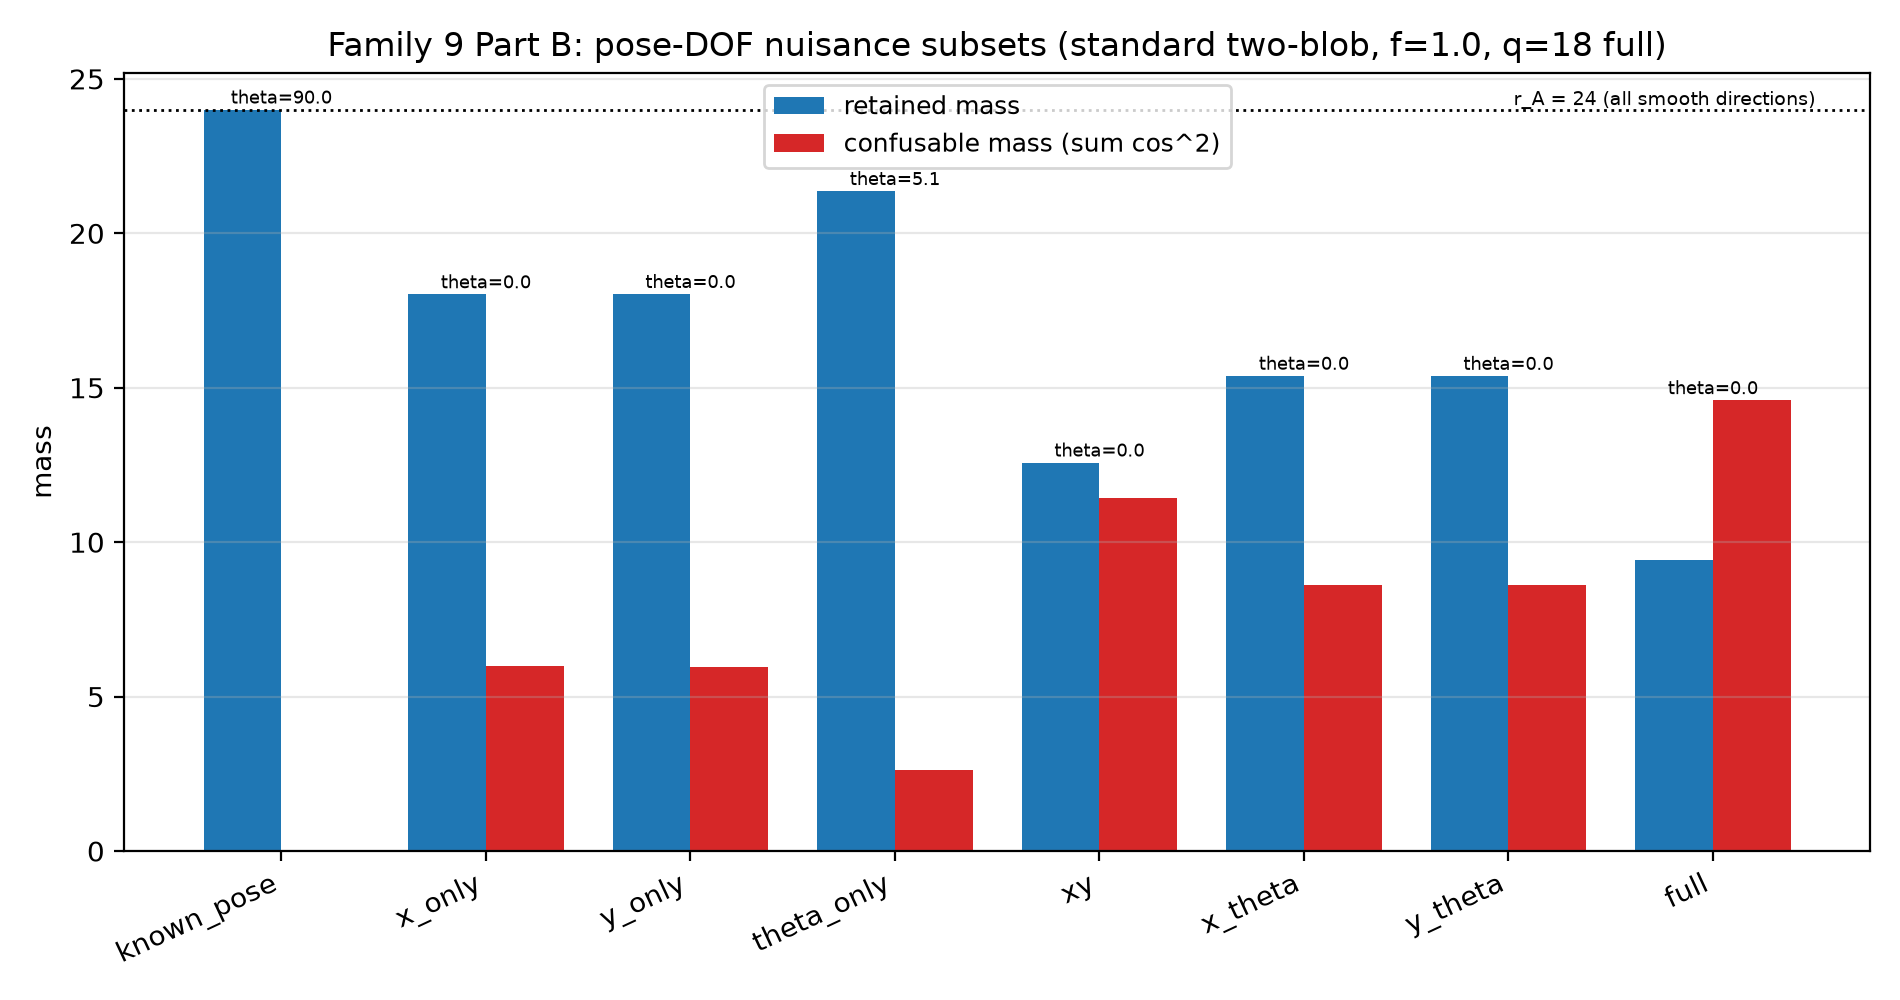
\includegraphics[width=0.86\textwidth]{../figures/family9_pose_dof_ablation.png}
\caption{Family 9 pose-DOF nuisance ablation.}
\label{fig:f9_dof}
\end{figure}

\begin{figure}[htbp]
\centering
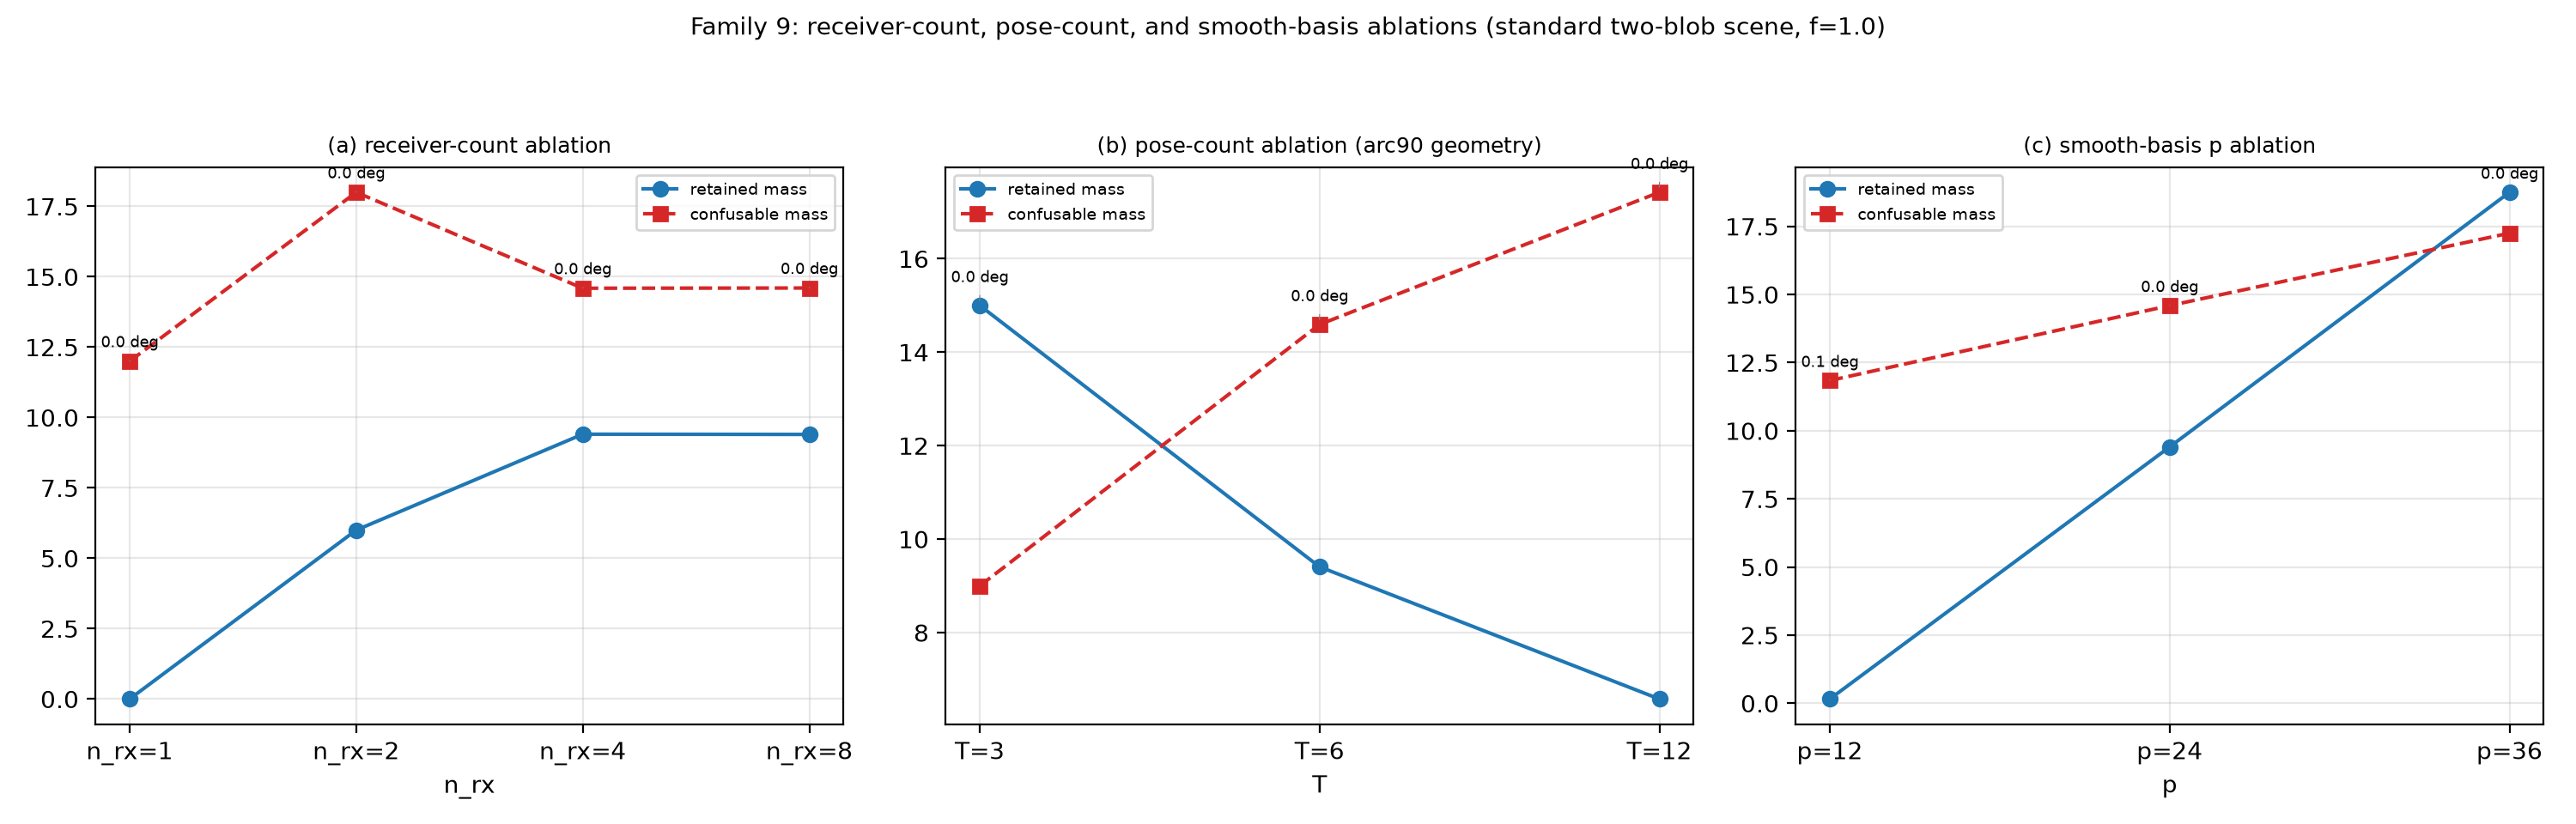
\includegraphics[width=0.86\textwidth]{../figures/family9_rx_T_basis_ablation.png}
\caption{Family 9 receiver-count, pose-count, and basis ablations.}
\label{fig:f9_rx}
\end{figure}

\subsection{Derived operator-Lipschitz bound (Family 5b2)}\label{sec:family5b2}

Family 5b2 corrects the loose structural bound of Family 5b and derives an
alpha-aware tight bound for the affine tangent model. The earlier family
replaced $\|C^{-1}\|_2$ by the alpha-agnostic quantity
$1/\sigma_{\min}(B)^2$, meaningful only when $B$ has full column rank, which
blew up as $\sigma_{\min}^{-4}$ despite
$\alpha=1.0$; the Family 5b constant $L_{\mathrm{struct}}=1.408\times10^7$ is
cited here only as corrected. Family 5b2 uses the exact
$\|C^{-1}\|_2=1/(\sigma_{\min}(B)^2+\alpha)$ for the PSD-plus-shift
$C=B^TB+\alpha I$ \FDL{}, extends the affine certificate to every
$\epsilon\ge0$ (the $\alpha$ floor keeps $C_{\mathrm{aff}}$ invertible), and
evaluates the actual radius-$\epsilon$ Lipschitz quotient on
$d=\epsilon u$.

\begin{table}[htbp]
\centering
\small
\caption{Family 5b2 tight Lipschitz ingredients and affine certificate
(\texttt{results/family5b2\_alpha\_tight.json}).}
\label{tab:f5b2}
\begin{tabular}{p{0.38\textwidth} p{0.54\textwidth}}
\toprule
quantity & value \\
\midrule
pointwise $L_{\mathrm{struct,tight}}(X_0)$ &
$1.124\times10^{-2}$ \\
loose Family 5b $L_{\mathrm{struct}}(X_0)$ (corrected) &
$1.408\times10^7$; tightness ratio $1.252285\times10^9$ \\
term balance & A-term $1.097\times10^{-2}$ (97.53\%);
regularised B/P term $2.783\times10^{-4}$ (2.47\%) \\
affine certificate (2000 directions, seed 7171) &
valid for $\epsilon\in\{10^{-3},3\times10^{-3},10^{-2},3\times10^{-2},10^{-1}\}$; \\
 & all fro/lambda checks true; $L_{\mathrm{cert,affine}}$ from
$1.131\times10^{-2}$ to $1.831\times10^{-2}$ \\
full nonlinear samples (500 directions, seed 9191) &
worst Frobenius quotient $3.228\times10^{-4}<L_{\mathrm{struct,tight}}(X_0)$; \\
 & no sampled violations; sampled envelope $1.125\times10^{-2}$ \\
FD Jacobian validation & global rel.\ Fro J$_A$ $5.991\times10^{-7}$,
J$_B$ $5.374\times10^{-7}$; O($h^2$) ratios $\sim4$ \\
\bottomrule
\end{tabular}
\end{table}

The tight pointwise constant is $L_{\mathrm{struct,tight}}(X_0)=1.124\times10^{-2}$,
an improvement by factor $1.252285\times10^9$ over the loose Family 5b value
of $1.408\times10^7$, and the balance reverses: the $A$-term supplies 97.53\%
of the tight constant while the regularised $B/P$ term contributes only
2.47\%. The affine tangent certificate is rigorous for the affine model
conditional on the numerically checked finite-difference Jacobians \FDL{}:
with $\alpha>0$, $C_{\mathrm{aff}}$ remains invertible for every
$\epsilon$ in the tested set up to $0.1$, and none of the 2000-direction
frobenius or eigenvalue-drop checks violates the certificate. The full
nonlinear model has no sampled violations either, but that result is a
derived structural bound with a sampled ingredient envelope, not a formal
nonlinear interval certificate \OBS{}: no uniform radius-$\epsilon$ bounds
on the nonlinear ingredients are proven.

\begin{figure}[htbp]
\centering
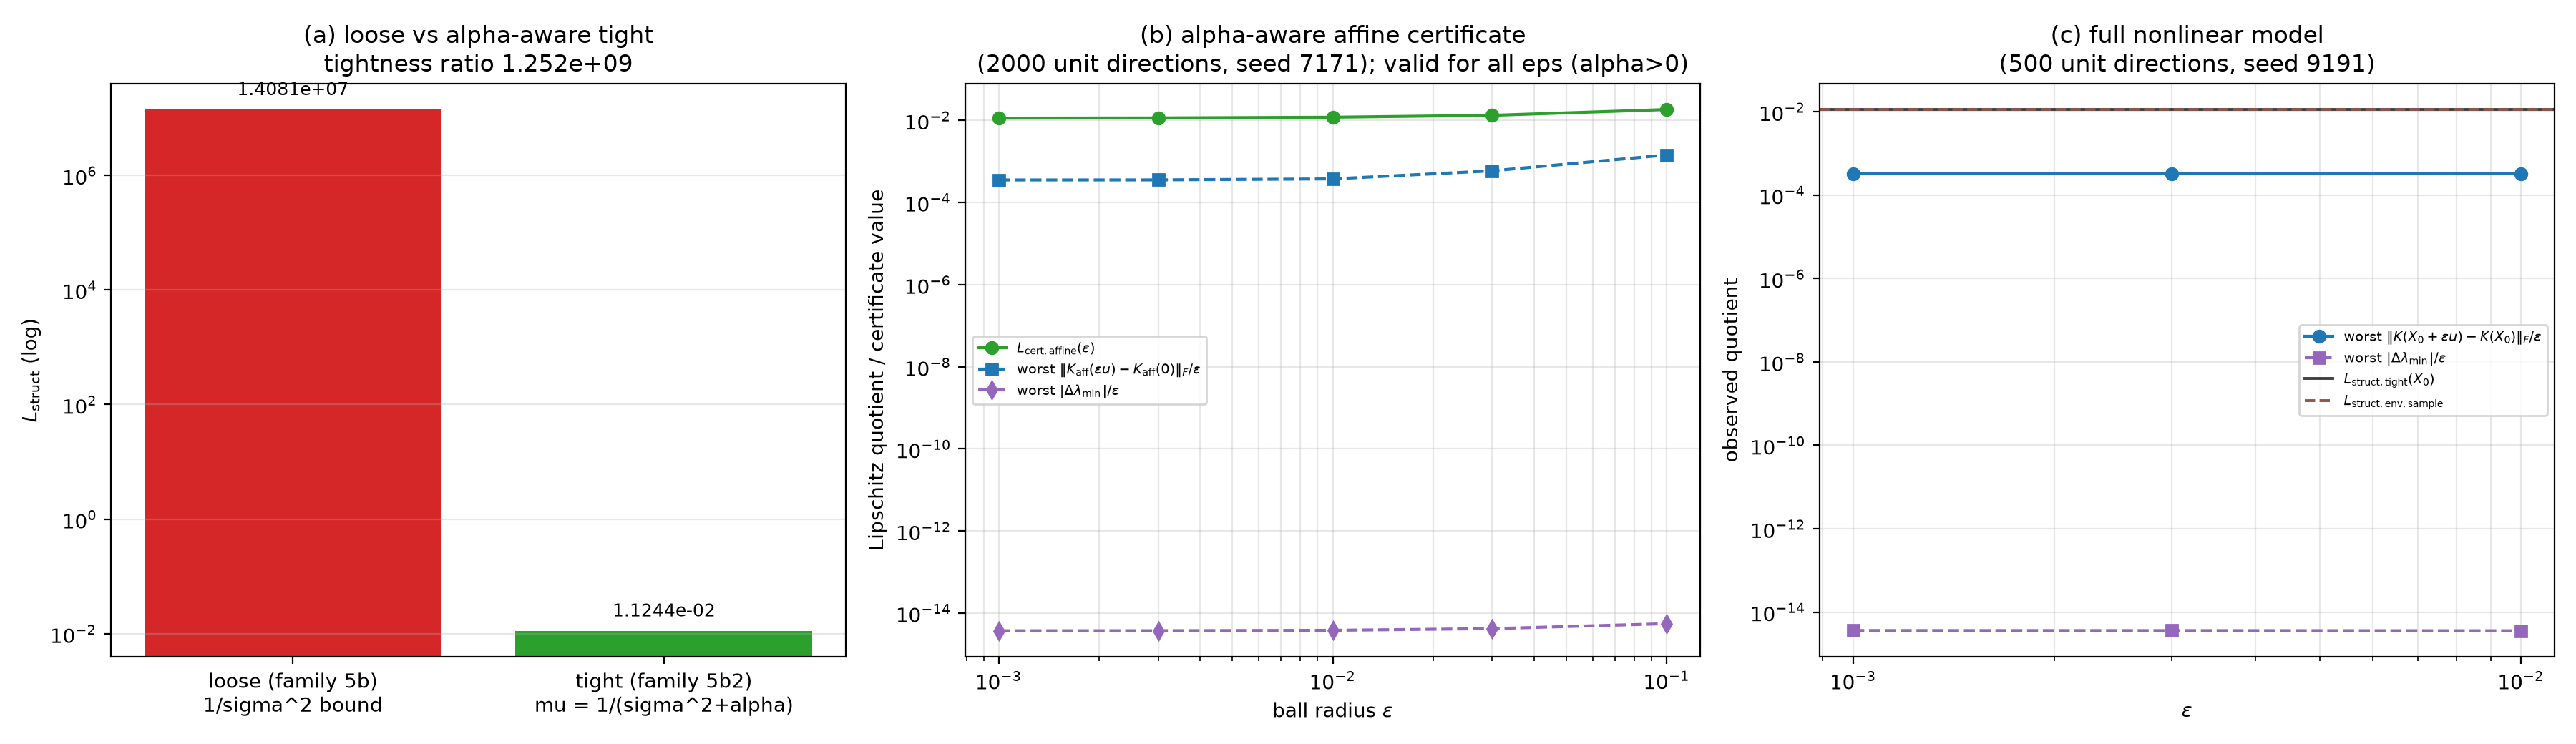
\includegraphics[width=0.86\textwidth]{../figures/family5b2_alpha_tight.png}
\caption{Family 5b2 alpha-aware tight Lipschitz certificate.}
\label{fig:f5b2}
\end{figure}

\subsection{Protocol-corrected NLS covariance toy (Family 10)}\label{sec:family10}

Family 10 runs a finite-dimensional nonlinear-least-squares covariance toy on
the multi-frequency (f=1.0/1.4/1.8), whitened/realified stacks
($A_{\mathrm{stack}}$ $144\times24$, $B_{\mathrm{stack}}$ $144\times18$,
$\alpha=1.0$, SNR=100) with 120 matched noise trials
(\path{results/family10_online_slam_toy_n120.json}). The protocol
correction of 2026-09-03 (\path{notes/family10_protocol_correction.md}) is
binding: the Monte Carlo scheme draws only data noise and keeps the true pose
fixed at $dx=0$ on every trial, so the correct linearized frequentist target
for the map component of the penalized free-pose estimator is the sandwich
covariance
\[
P_{\mathrm{samp}}=[H^{-1}H_{\mathrm{data}}H^{-1}]_{1:p,1:p},\qquad
H_{\mathrm{data}}=\begin{bmatrix}K_{\mathrm{IS}}&A^TB\\(A^TB)^T&B^TB\end{bmatrix},
\qquad H=H_{\mathrm{data}}+\mathrm{diag}(0_p,\alpha I_q),
\]
not the Bayesian marginal $K_{\mathrm{eff}}^{-1}$. $K_{\mathrm{eff}}^{-1}$ is
the posterior/prior-consistent map marginal and is realized empirically only
when each trial draws its own pose from the prior; the original comparison
against it is therefore retained as a protocol-correction/negative result.

\begin{table}[htbp]
\centering
\small
\caption{Family 10 key numbers
(\texttt{results/family10\_online\_slam\_toy\_n120.json};
corrected sandwich ratios from \texttt{notes/family10\_protocol\_correction.md}
recomputed from the stored theory spectra).}
\label{tab:f10}
\begin{tabular}{p{0.36\textwidth} p{0.56\textwidth}}
\toprule
quantity & value (Born / full-wave) \\
\midrule
empirical rel.\ Fro deviation vs $P_{\mathrm{known}}$ (known pose) &
$0.0779$ / $0.474$ (known successes 120/120, 120/120) \\
empirical rel.\ Fro deviation vs $P_{\mathrm{free}}=K_{\mathrm{eff}}^{-1}$ &
$13.49$ / $4.04$ (free successes 115/120, 119/120) \\
predicted retained DOF $\mathrm{tr}(K_{\mathrm{eff}}K_{\mathrm{IS}}^{-1})$ &
$14.03$ / $14.37$ \\
trace ratio, old target $\mathrm{tr}(P_{\mathrm{free}})/\mathrm{tr}(P_{\mathrm{known}})$ &
$6.07$ / $3.63$ \\
trace ratio, empirical free-pose sample &
$82.9$ / $11.0$ \\
trace ratio, corrected sandwich target
$\mathrm{tr}(P_{\mathrm{samp}})/\mathrm{tr}(P_{\mathrm{known}})$ &
$3.889$ / $2.755$ (Born affine control
\texttt{family10\_affine\_control.json}: $3.8888$) \\
directional FD self-check of the stacked residual Jacobian &
Born $7.70\times10^{-10}$; full-wave batch rel.\ Fro
$4.66\times10^{-10}$ (eps=$10^{-6}$) \\
\bottomrule
\end{tabular}
\end{table}

The known-pose comparison is close for Born ($0.0779$) and only qualitative
for full wave ($0.474$), whose data model is not affine in the map
coefficients. The free-pose comparison is a mismatch under either target: the
stored deviations against the old $P_{\mathrm{free}}$ target are $13.49$
(Born) and $4.04$ (full wave), and correcting the target to $P_{\mathrm{samp}}$
makes the Born discrepancy larger rather than smaller: the protocol-correction
recomputation reports relative Frobenius deviations of $22.0$ (Born) and $5.40$
(full wave) against the corrected $P_{\mathrm{samp}}$ target.
Interpretation, recorded as written: first-order spectral predictions track
the known-pose full-wave uncertainty only qualitatively; the free-pose and
most-confounded directions carry large sampling variance, and the linearized
free-pose covariance does not match the empirical $P_{\mathrm{samp}}$ at the
tested 120 trials. This is explicitly a finite-dimensional NLS toy on the
recorded N=16 geometry; it is not an online SLAM system claim and no
estimator optimality or global-convergence property is asserted.

\begin{figure}[htbp]
\centering
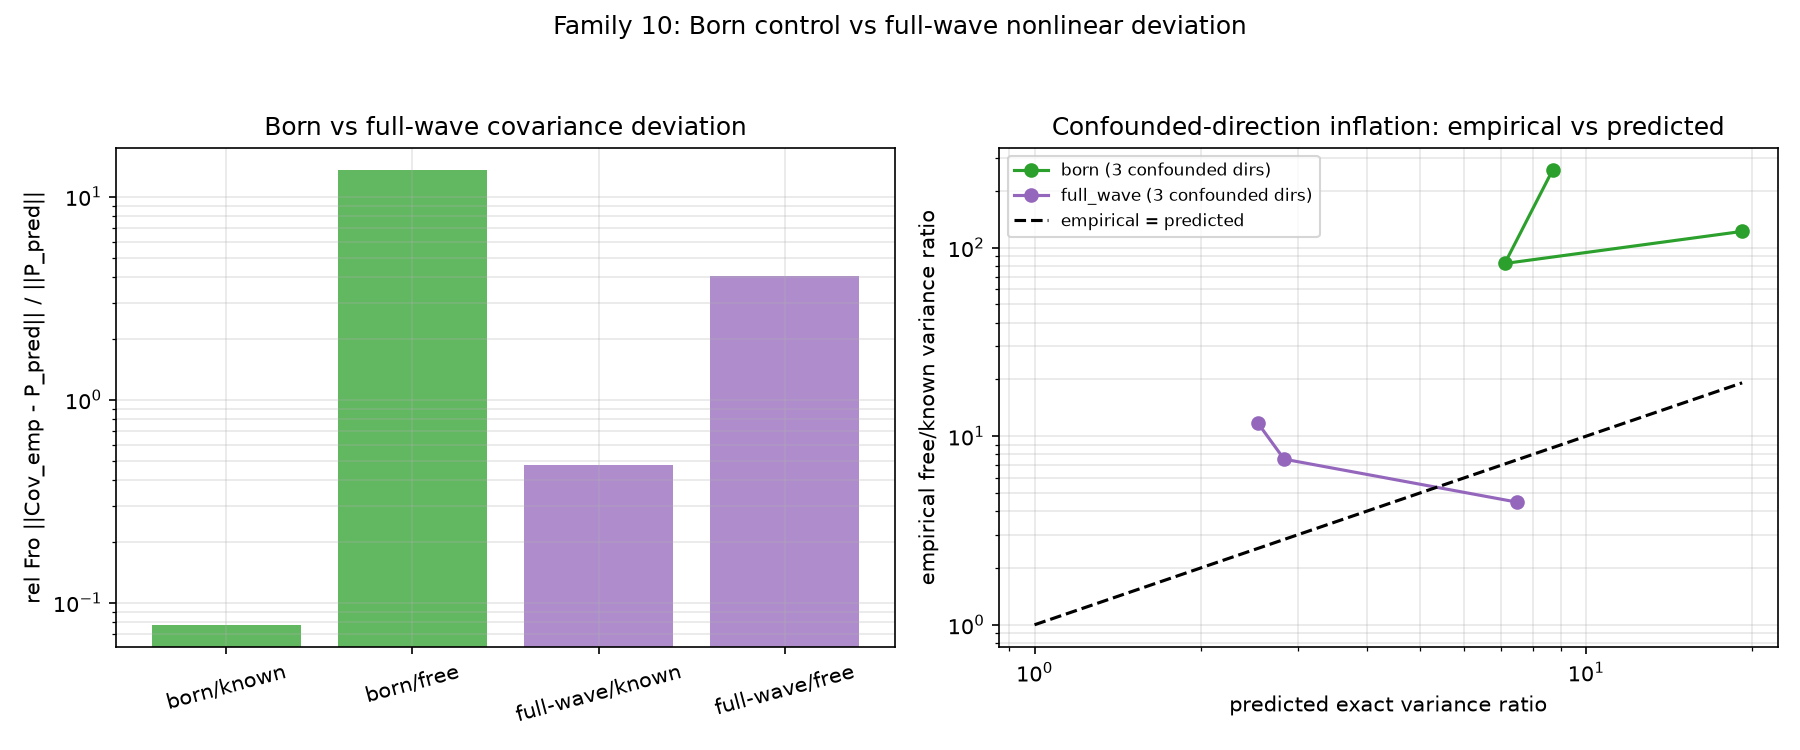
\includegraphics[width=0.86\textwidth]{../figures/family10_born_vs_fullwave_deviation_n120.png}
\caption{Family 10 stored Born and full-wave empirical-versus-predicted
covariance deviations at n=120.}
\label{fig:f10_deviation}
\end{figure}

\begin{figure}[htbp]
\centering
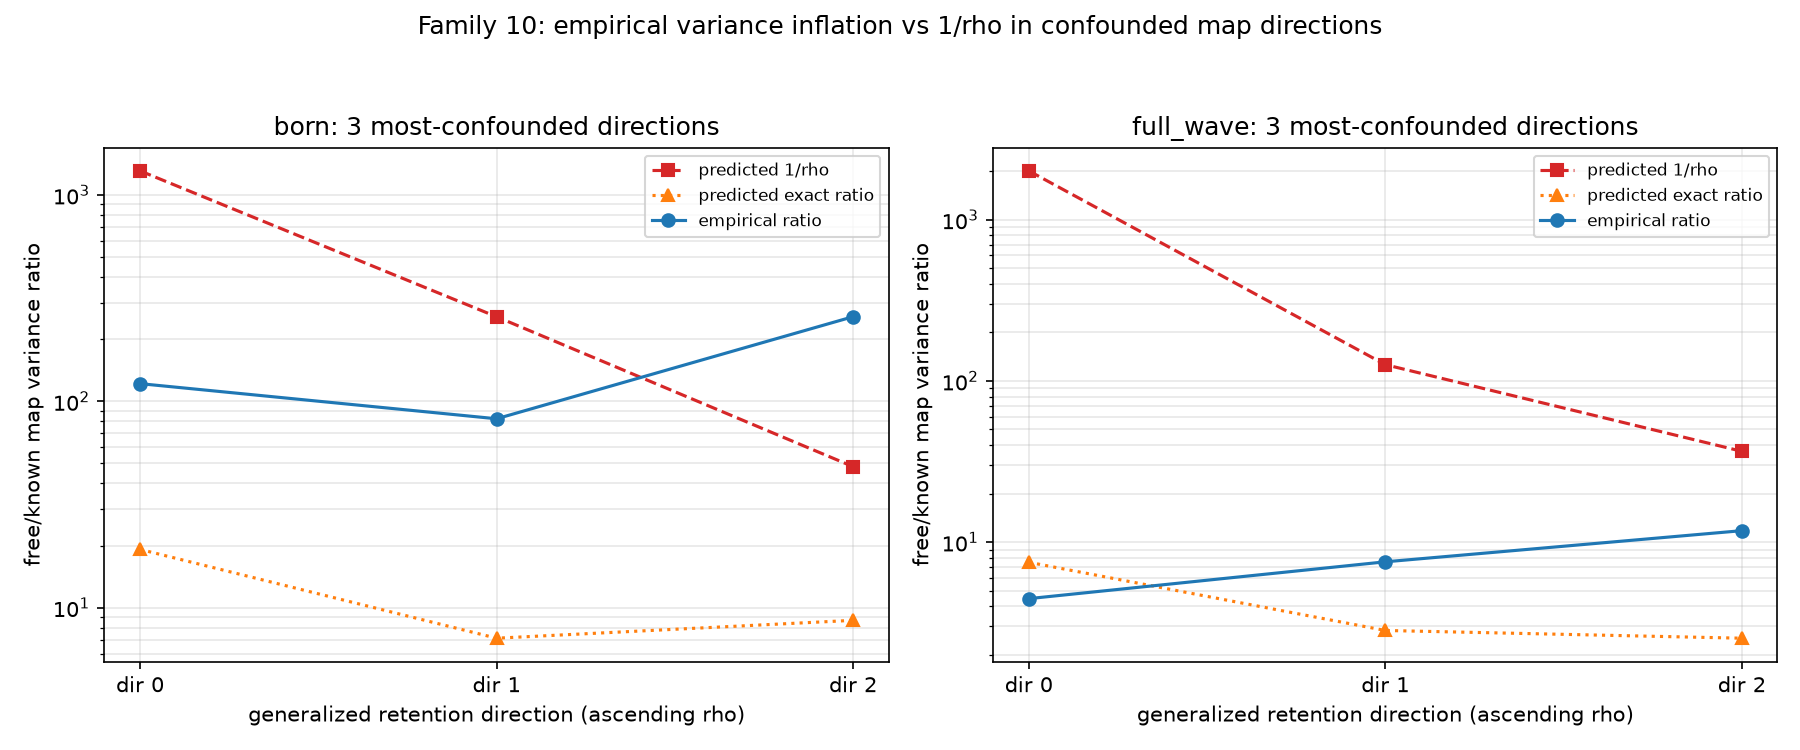
\includegraphics[width=0.86\textwidth]{../figures/family10_confounded_direction_ratios_n120.png}
\caption{Family 10 most-confounded direction variance ratios at n=120.}
\label{fig:f10_direction}
\end{figure}

\begin{figure}[htbp]
\centering
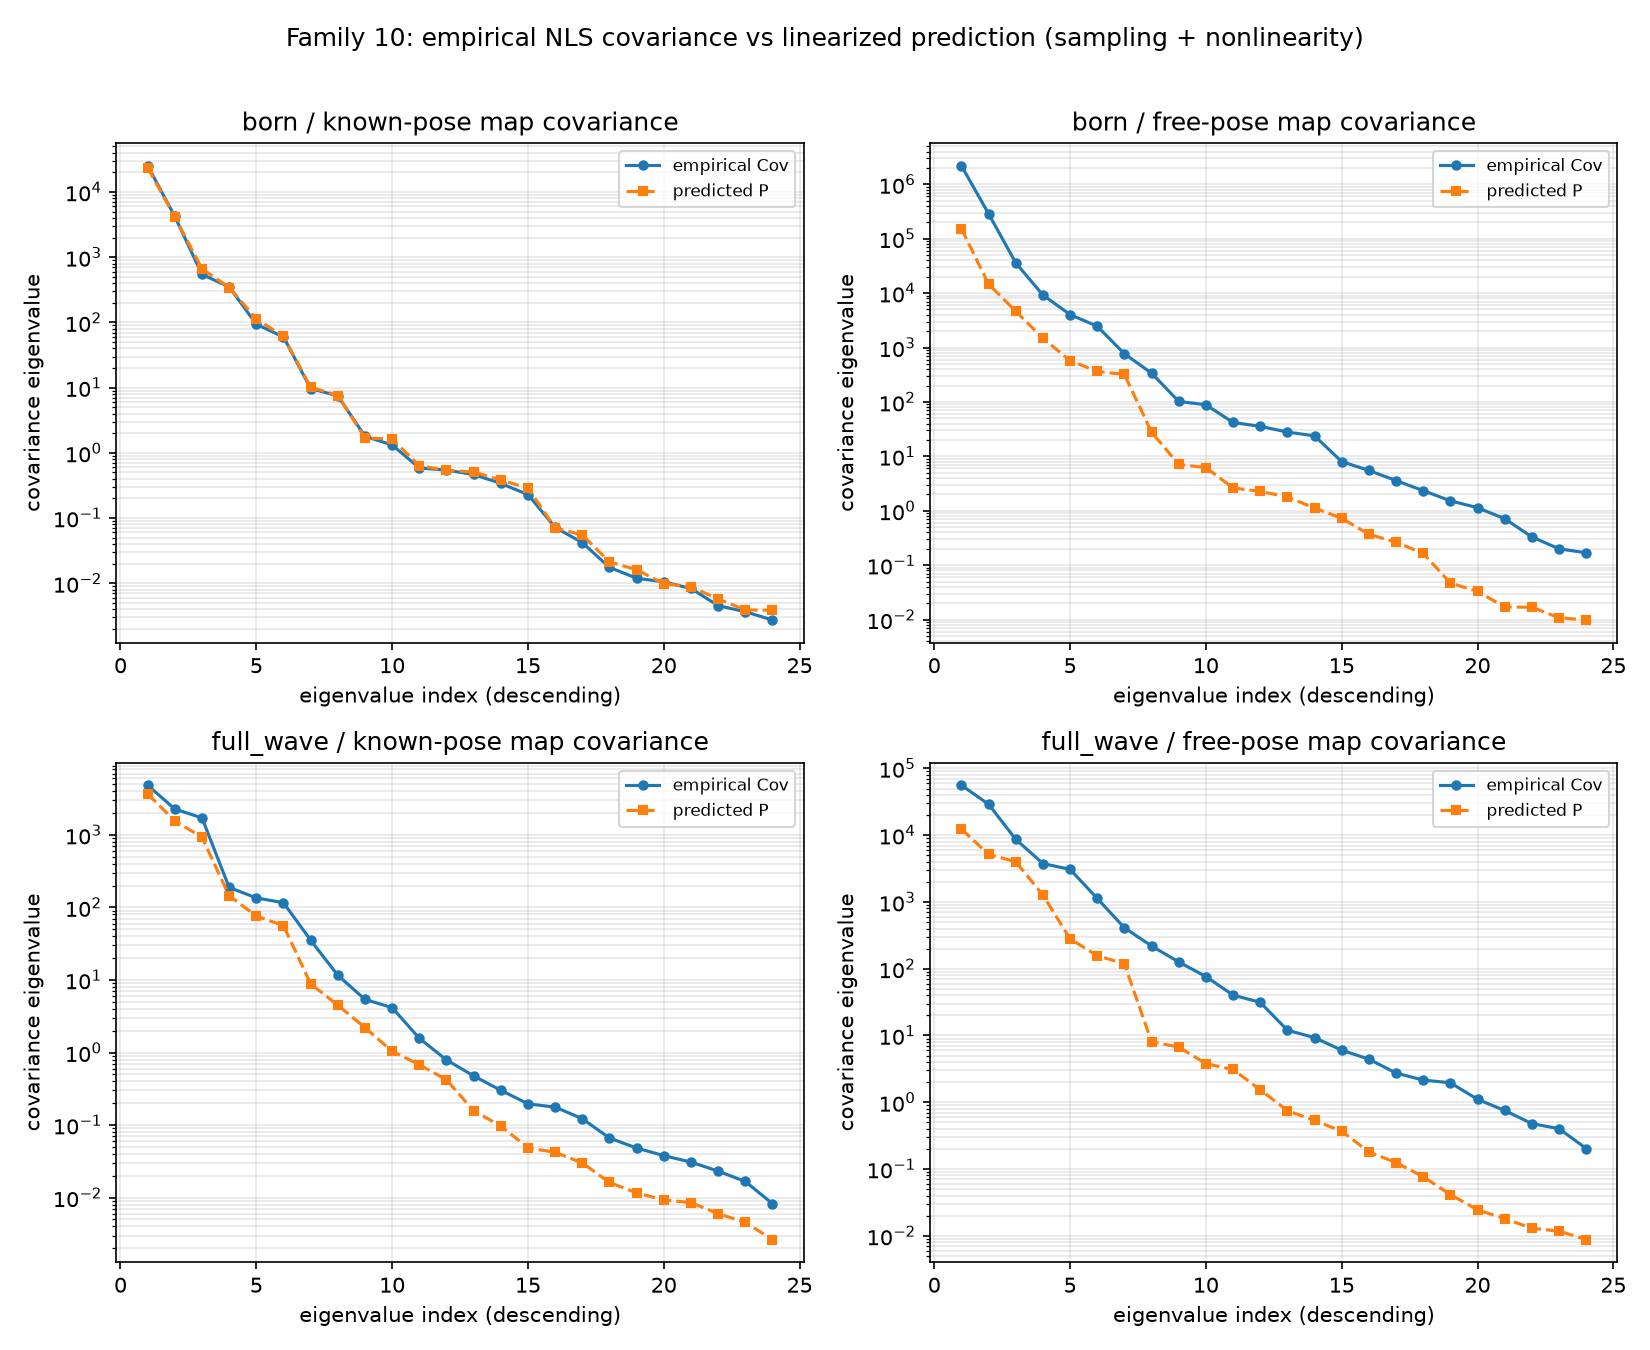
\includegraphics[width=0.86\textwidth]{../figures/family10_cov_eigenvalues_n120.png}
\caption{Family 10 predicted and empirical covariance spectra at n=120.}
\label{fig:f10_spectra}
\end{figure}

\subsection{SNR/frequency-set replication across scenes (Family 11)}\label{sec:family11}

Family 11 (\texttt{results/family11\_snr\_diversity.json}) replicates the
Family 4/6 non-monotone SNR curve --- movement of the three most
pose-confounded single-frequency directions as a second frequency's SNR
varies, including a finite positive high-SNR plateau --- over three scenes
(two\_blob, ring, low\_contrast) at f2=1.4 and f2=1.8, then records equal-SNR
frequency-set stacks (F1/F2/F3/F5), duplicate-block controls, and a
fixed-count bandwidth sweep. All rows are deterministic N=16 dense linear
algebra under the declared SNR-whitened model; no forced pass is applied.

\begin{table}[htbp]
\centering
\small
\caption{Family 11 replication and equal-SNR frequency-set rows. Retained DOF
is $\sum\rho$ of the generalized $K_{\mathrm{eff}}$-versus-$K_{\mathrm{IS}}$
retention spectrum at $\alpha=1$.}
\label{tab:f11}
\begin{tabular}{p{0.36\textwidth} p{0.56\textwidth}}
\toprule
replication cell & non-monotone directions; peak+plateau \\
\midrule
two\_blob, f2=1.4 & 3/3; replicates; peaks at snr$_2$=100 \\
two\_blob, f2=1.8 & 3/3; replicates; peaks at snr$_2$=316--1000 \\
ring, f2=1.4 & 3/3; replicates; peaks at snr$_2$=316--1000 \\
ring, f2=1.8 & 3/3; replicates; peaks at snr$_2$=316--1000 \\
low\_contrast, f2=1.4 & 3/3; replicates; peaks at snr$_2$=31.6--316 \\
low\_contrast, f2=1.8 & 2/3; exception: u1 has no interior peak
(monotone rise into tail) \\
\midrule
equal-SNR retained DOF (F1/F2/F3/F5) &
two\_blob 11.29 / 13.48 / 15.64 / 15.91; ring 15.84 / 17.99 / 19.26 / 20.06;
low\_contrast 16.98 / 17.11 / 18.62 / 18.96 \\
\midrule
bandwidth retained DOF (narrow/mid/wide) &
two\_blob 14.71 / 15.64 / 14.52; ring 18.80 / 19.26 / 18.61;
low\_contrast 17.97 / 18.62 / 18.06; mid band gives the largest retained DOF
and least-negative positive-support log-pseudovolume in every tested scene \\
\bottomrule
\end{tabular}
\end{table}

\begin{table}[htbp]
\centering
\small
\caption{Family 11 duplicate-block invariance under the jointly scaled prior.}
\label{tab:f11dup}
\begin{tabular}{p{0.21\textwidth} p{0.25\textwidth} p{0.23\textwidth} p{0.20\textwidth}}
\toprule
scene & max movement & no-prior rel.\ DOF diff &
joint-prior gate \\
\midrule
two\_blob & $1.256\times10^{-16}$ & $4.305\times10^{-14}$ & PASS ($<10^{-10}$) \\
ring & $2.682\times10^{-16}$ & $7.832\times10^{-15}$ & PASS ($<10^{-10}$) \\
low\_contrast & $2.187\times10^{-16}$ & $3.699\times10^{-13}$ & PASS ($<10^{-10}$) \\
\bottomrule
\end{tabular}
\end{table}

Equal-SNR frequency sets grow retained DOF with set size on all three scenes
\OBS{}, and duplicate-block invariance holds under the jointly scaled prior
\FDL{} with every reported gate below $10^{-10}$. The fixed-count bandwidth
sweep is non-monotone: the mid band (1.0--1.4--1.8) gives the largest retained
DOF and least-negative positive-support log-pseudovolume on all three tested
scenes, with both the narrow and wide bands lower. Here the latter is the
thresholded sum of $\log\rho_i$ over recorded positive retentions, not an
unqualified full-rank log-determinant. The replication statement is deliberately
qualified: frequency diversity is real in this finite-dimensional model but is
finite-dimensional and scene-specific. In particular, low\_contrast at f2=1.8
replicates only 2/3 directions (direction u1 rises monotonically into its tail
without an interior peak) and is recorded as a scene-specific exception, not a
universal rule.

\begin{figure}[htbp]
\centering
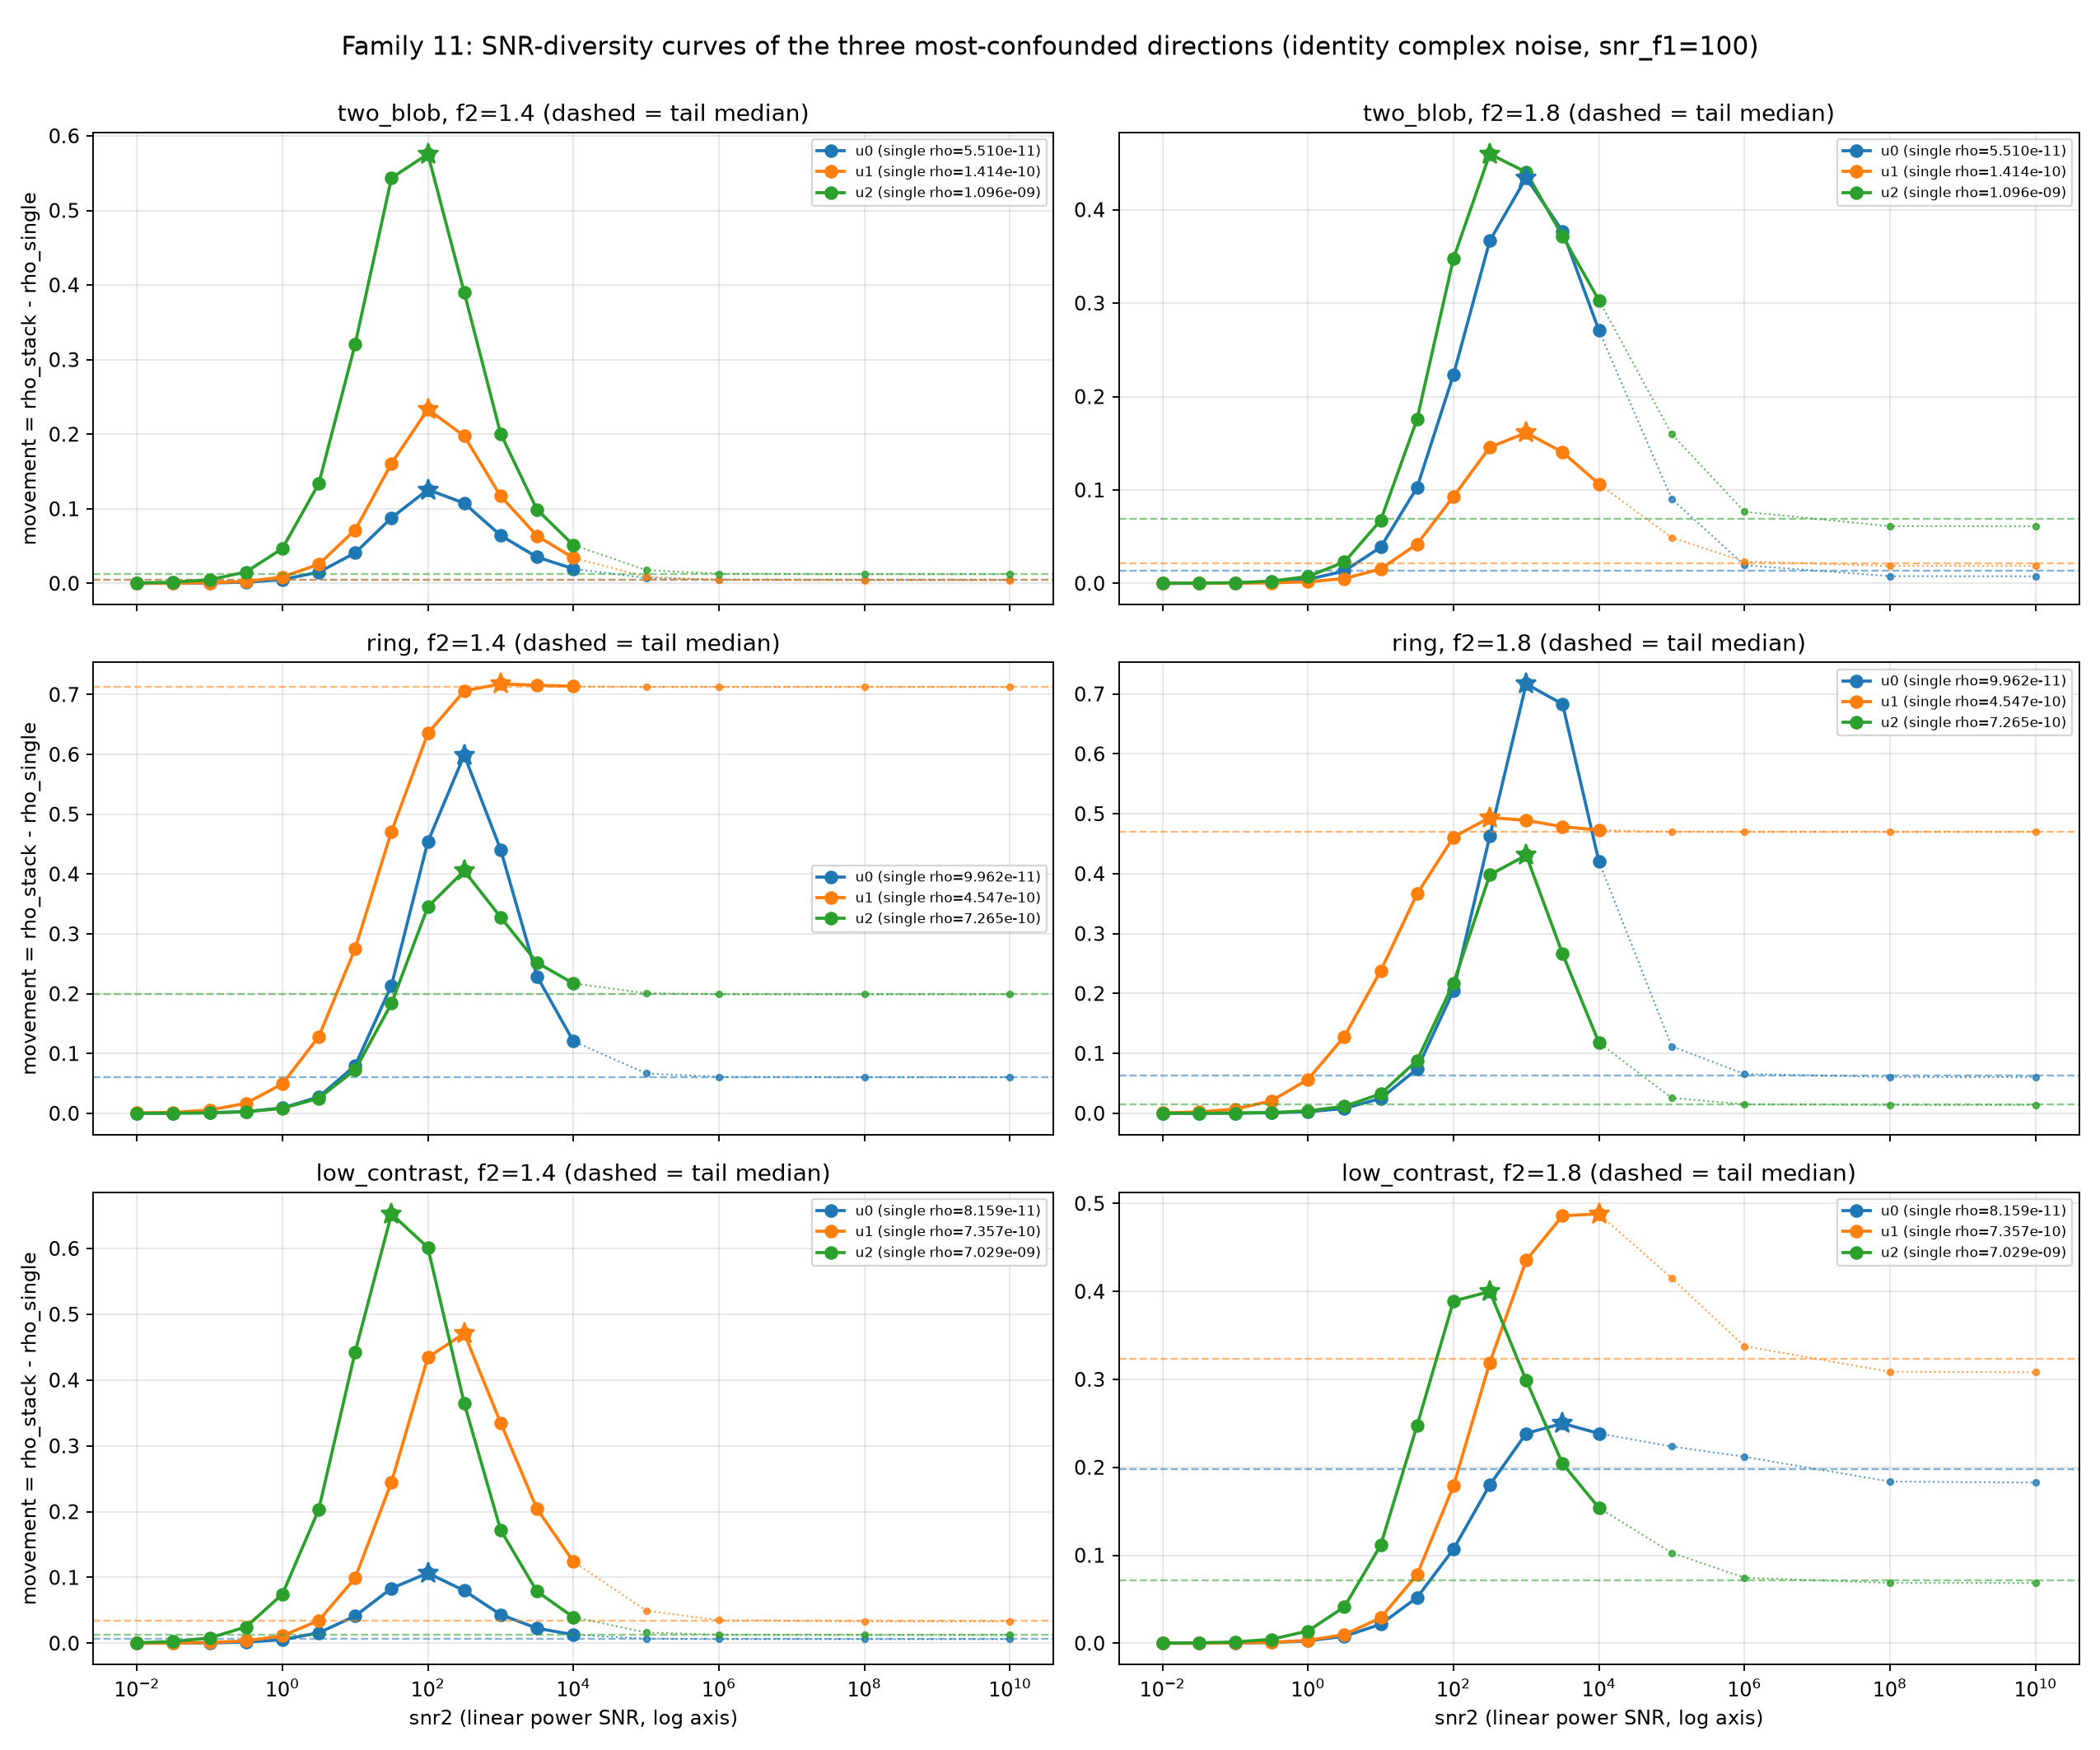
\includegraphics[width=0.86\textwidth]{../figures/family11_snr_sweep_scenes.png}
\caption{Family 11 non-monotone SNR curves across scenes and f2 values.}
\label{fig:f11_snr}
\end{figure}

\begin{figure}[htbp]
\centering
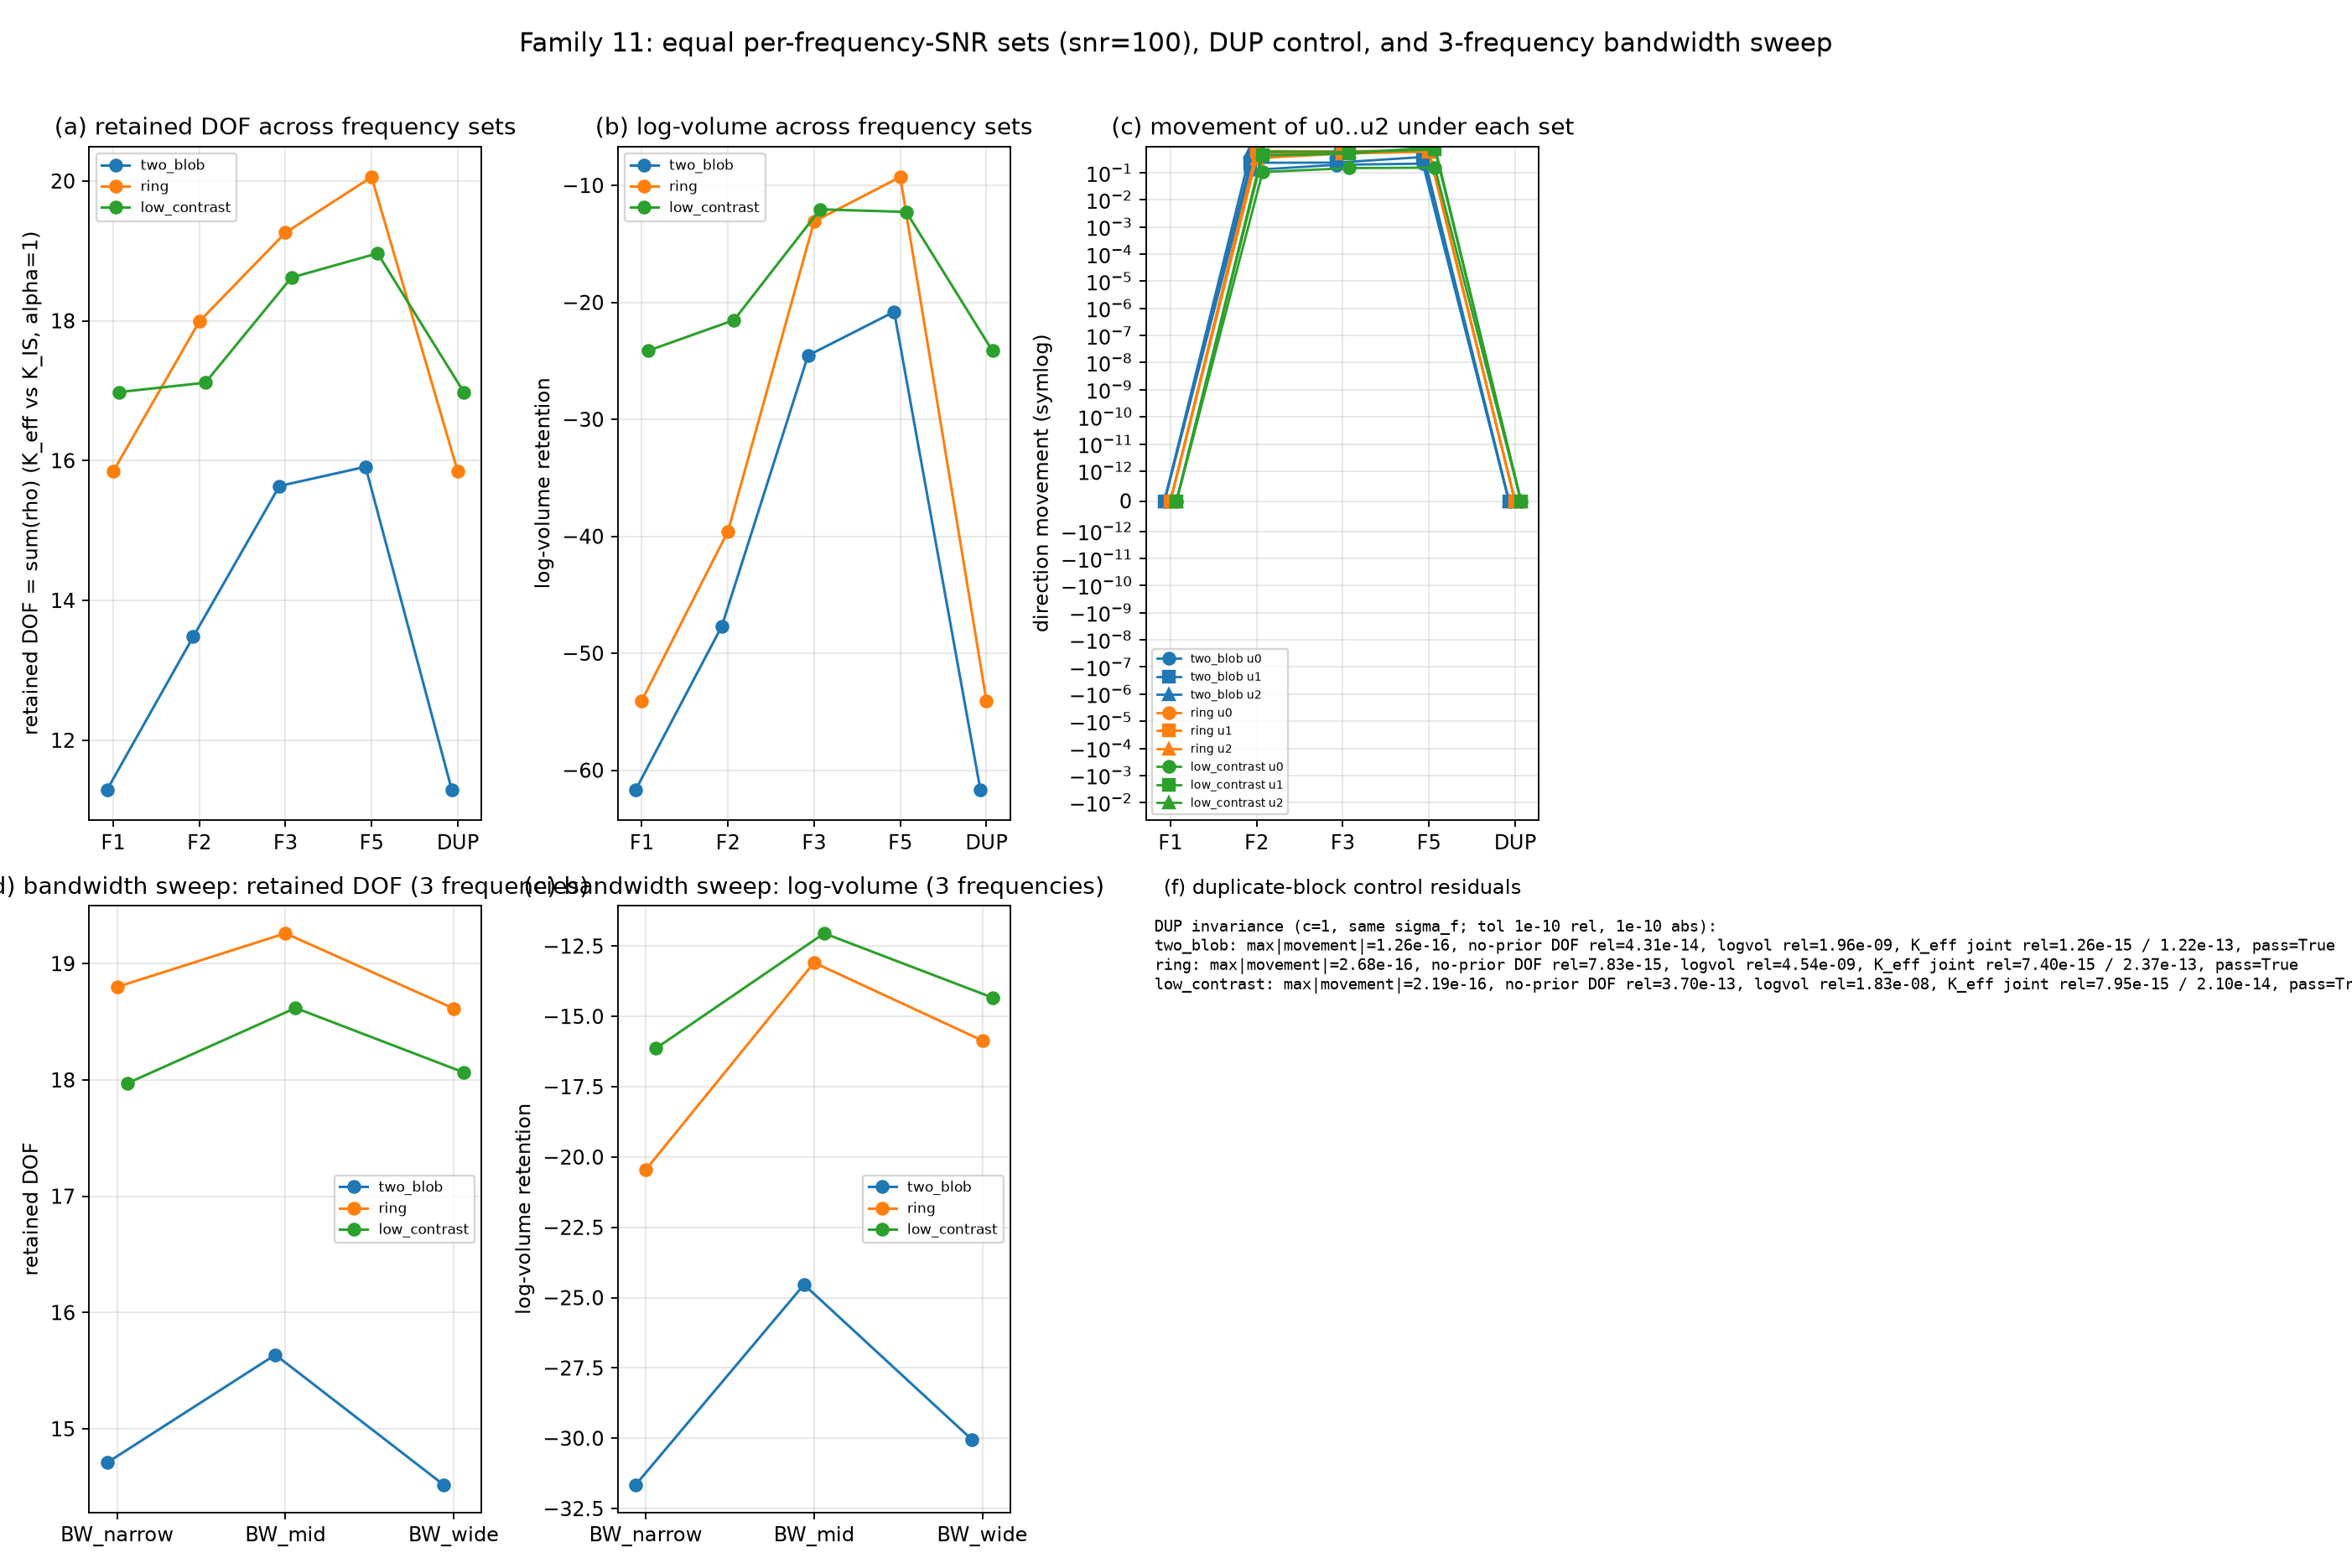
\includegraphics[width=0.86\textwidth]{../figures/family11_frequency_sets.png}
\caption{Family 11 equal-SNR frequency-set and bandwidth rows.}
\label{fig:f11_sets}
\end{figure}

\subsection{Trajectory replication and mechanism (Family 12)}\label{sec:family12}

Family 12 (\texttt{results/family12\_trajectory\_replication.json}) recomputes
the Family 4/4c trajectory comparison over four scenes (two\_blob, ring,
low\_contrast, offset\_edge), two controls (A: raw equal-continuous-length;
B: same-standoff per-pose-energy-normalized), and three frequency sets
(F1/F2/F3), for straight, arc90, arc180, and circle360 (96 metric cells plus
24 ordering cells). The old hypothesis ordering (circle360 $>$ arc180 $>$ arc90
$>$ straight by retained DOF) holds in 0/24 (scene, control, frequency-set)
cells.

\begin{table}[htbp]
\centering
\small
\caption{Family 12 key numbers.}
\label{tab:f12}
\begin{tabular}{p{0.36\textwidth} p{0.56\textwidth}}
\toprule
quantity & value \\
\midrule
old hypothesis ordering holds & 0/24 cells (every cell false, no forced pass) \\
cross-check 1 (control B/F1/two\_blob vs Family 4c) &
PASS; max abs retained-DOF diff $2.978\times10^{-7}<3\times10^{-7}$ \\
cross-check 2 (control A/F1/two\_blob order) &
arc90 $>$ straight $>$ circle360 $>$ arc180; matches
\texttt{results/family4\_results.json}; the earlier checklist phrase
transposed arc180/circle360 \\
raw vs normalized orderings agree & 2/12 scene-frequency cells
(ring/F3, low\_contrast/F1) \\
c2 rank identity & 93/96 cells; exceptions ring/arc90/F1 (controls A and B,
residuals 3 and 1) and offset\_edge/arc90/F1 (control A, residual 1) \\
per-pose normalization verification & max $|1-\|A_{\mathrm{block}}\|_F|=
2.220446\times10^{-16}$ (gate $\le10^{-12}$) \\
$\mathrm{rank}(B)$ across all 96 cells & 18 in every cell \\
discrete total turning angle & straight 0, arc90 72, arc180 144,
circle360 240 deg \\
\bottomrule
\end{tabular}
\end{table}

\paragraph{Cross-checks and recorded checklist correction.}
Cross-check 1 reproduces the Family 4c normalized retained DOF for
control B/F1/two\_blob to within $3\times10^{-7}$ (PASS). Cross-check 2
recomputes the control A/F1/two\_blob ordering as
arc90 $>$ straight $>$ circle360 $>$ arc180, which matches the stored
\texttt{results/family4\_results.json} observed order; an earlier checklist
phrase (arc90 $>$ straight $>$ arc180 $>$ circle360) transposed
arc180/circle360 relative to that stored artifact, and the family-12 record
notes this without a forced pass. The Family 4 trajectory counterexample is
therefore preserved against the recorded artifact, not against the transposed
phrase.

\paragraph{Rank-identity exceptions.}
The c2 identity holds in 93/96 cells. The three exceptions are
single-frequency near-null rank-threshold observations (ring/arc90/F1 in
controls A and B, and offset\_edge/arc90/F1 in control A), where some
$K_{\mathrm{SLAM}}$ singular values fall below the Family-2 machine rank
tolerance at relative sizes $\sim10^{-13}$--$10^{-17}$; they are recorded as
numerical rank-threshold observations, not algebraic failures
(Section~\ref{sec:family13}).

\paragraph{Mechanism account (descriptive, no universal claim).}
$\mathrm{rank}(B)=18$ in every cell, so the ranking differences are not a
nuisance-rank effect. Shared pose-compensation residuals and per-pose
illumination differ across trajectories, and rankings shift with scene,
frequency set, and control: for example, two\_blob/F1 ranks
arc90 $>$ straight $>$ circle360 $>$ arc180 under control A but
arc90 $>$ straight $>$ arc180 $>$ circle360 under control B, while
two\_blob/F2 under control A places circle360 first. The discrete total
turning angle (0/72/144/240 deg for the four paths) alone does not explain the
rankings; raw and normalized orderings agree in only 2/12 cells. No universal
trajectory-ordering theorem is claimed \CTX{} for the universal hypothesis and
\OBS{} for the metric/scene/frequency dependence.

The angle panel below is computed only from the no-prior subspaces through the
singular values of $Q_B^TQ_A$. Any stored finite-prior quantity obtained by
applying $\arccos\sqrt{1-\rho}$ to a Schur-retention value is merely a
retention-angle transform and is not called a principal angle here.

\begin{figure}[htbp]
\centering
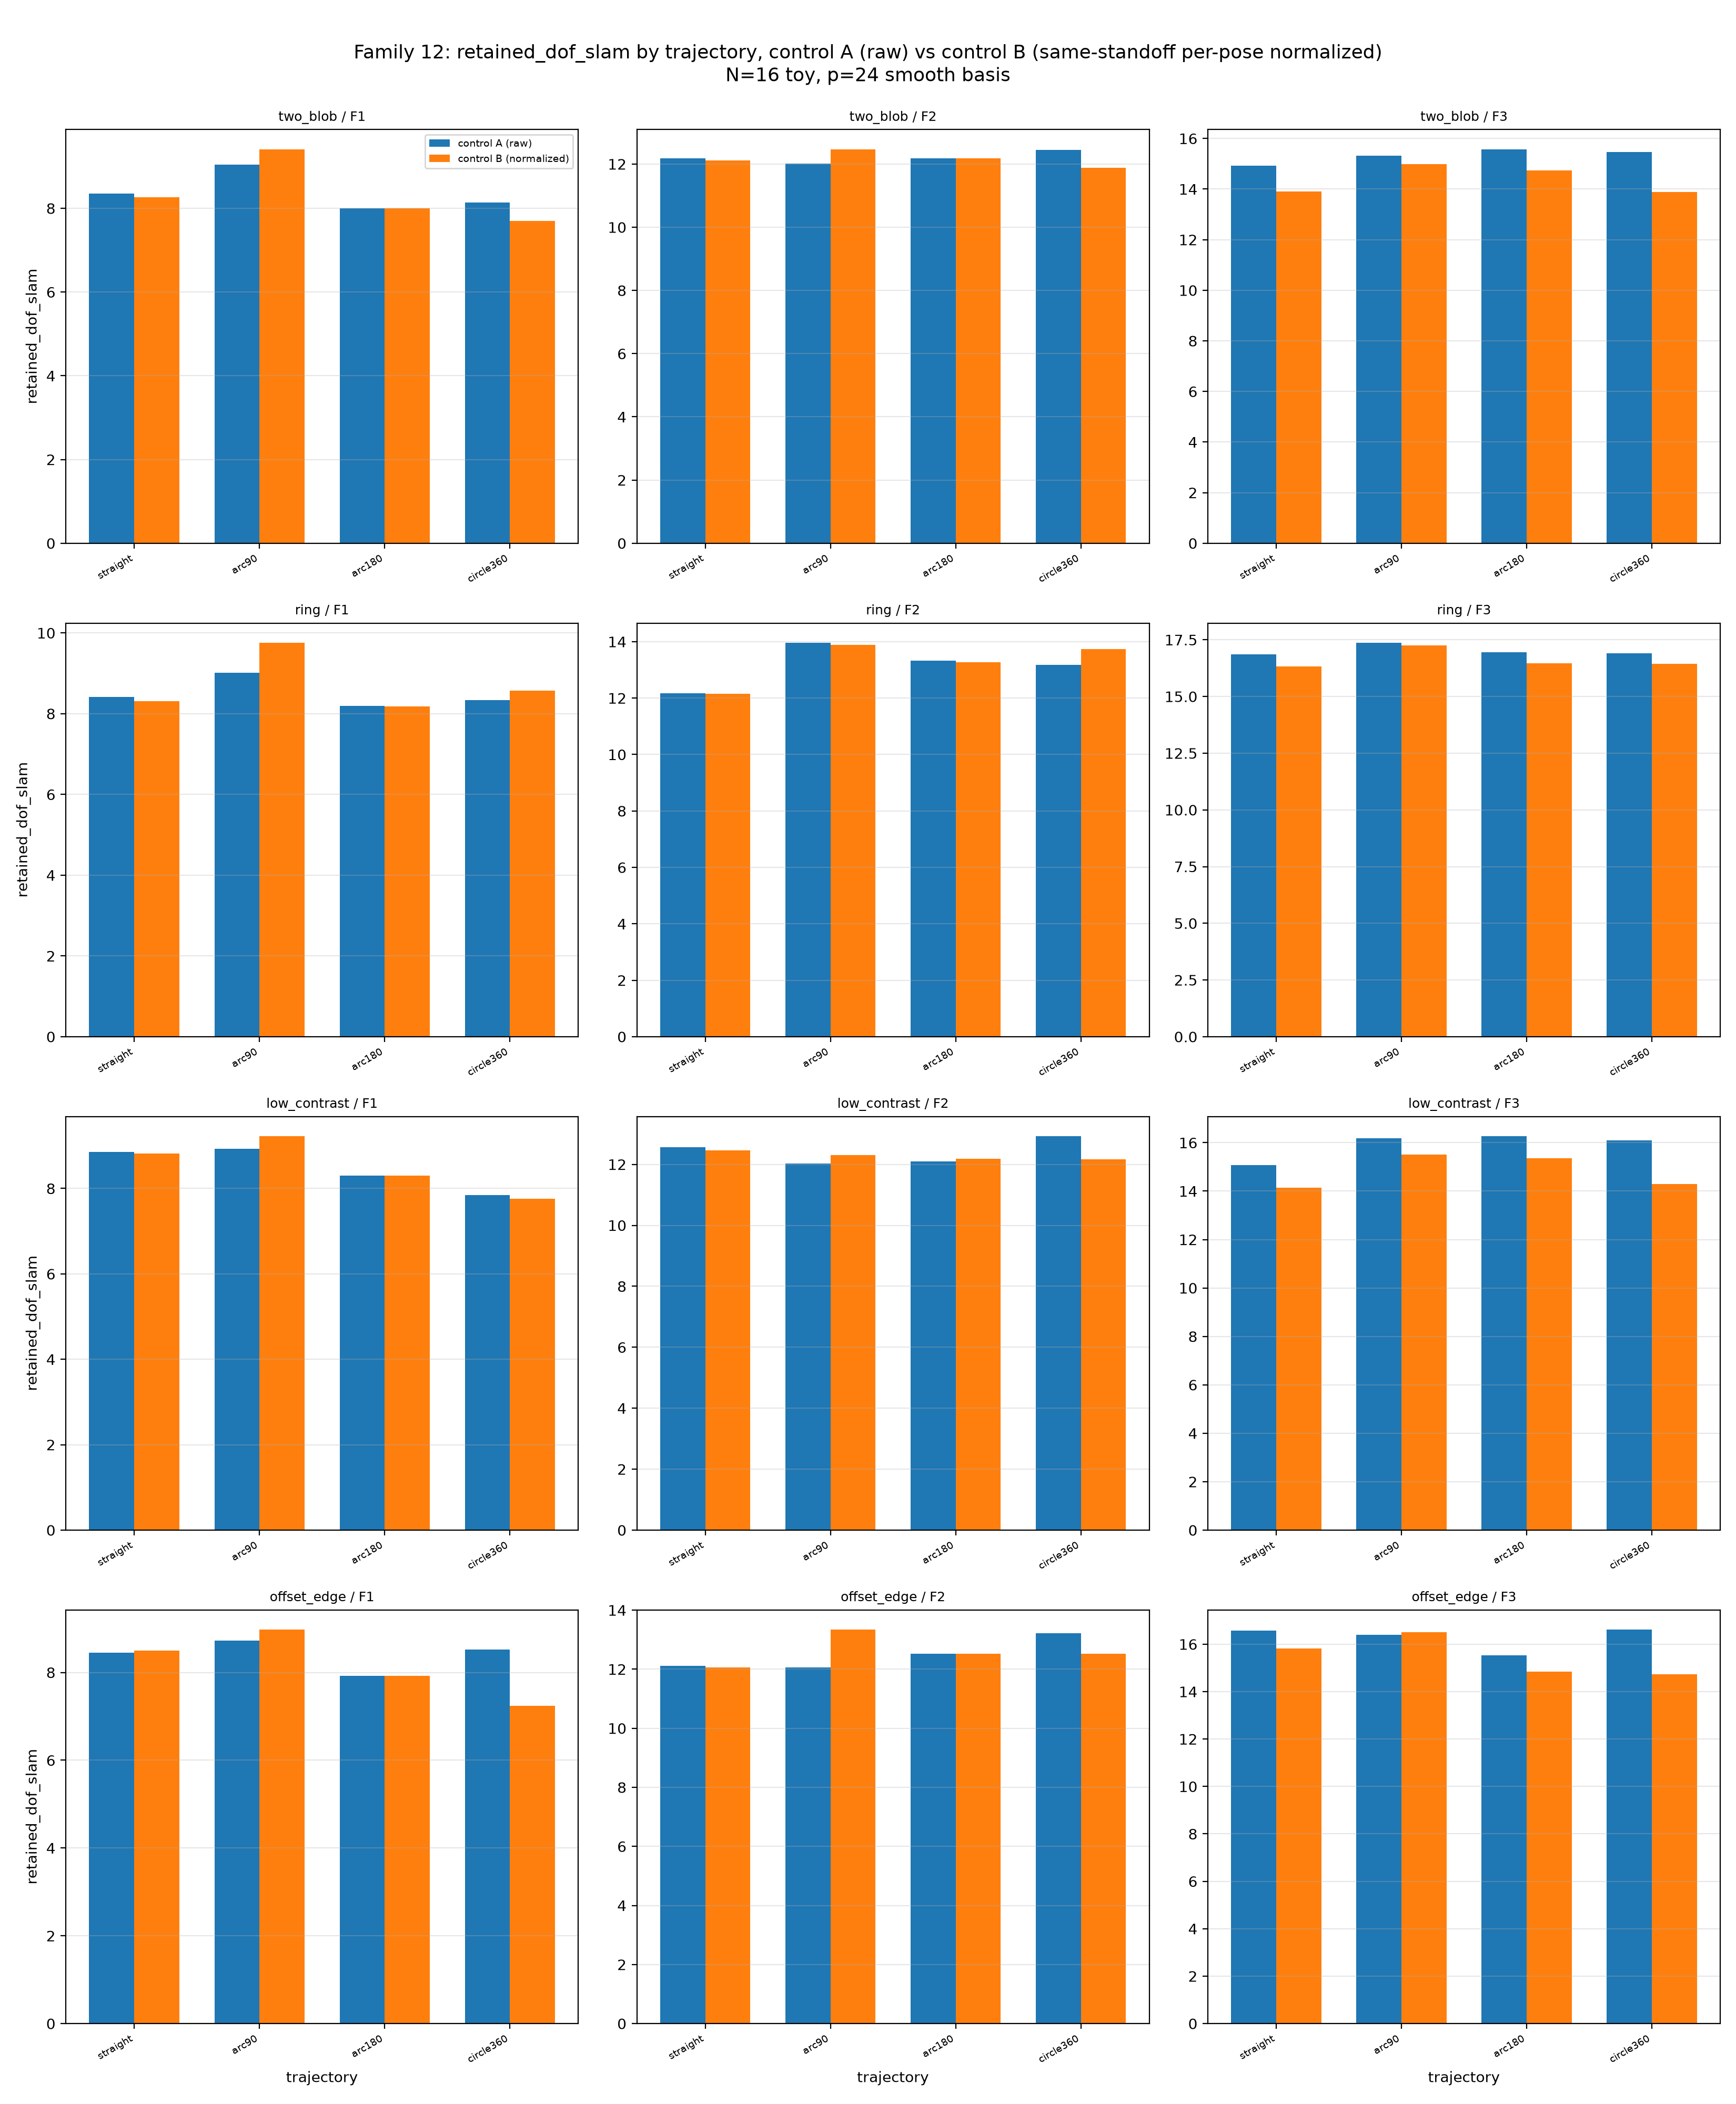
\includegraphics[width=0.86\textwidth]{../figures/family12_retained_rankings.png}
\caption{Family 12 retained-DOF rankings across scenes, controls, and
frequency sets.}
\label{fig:f12_rankings}
\end{figure}

\begin{figure}[htbp]
\centering
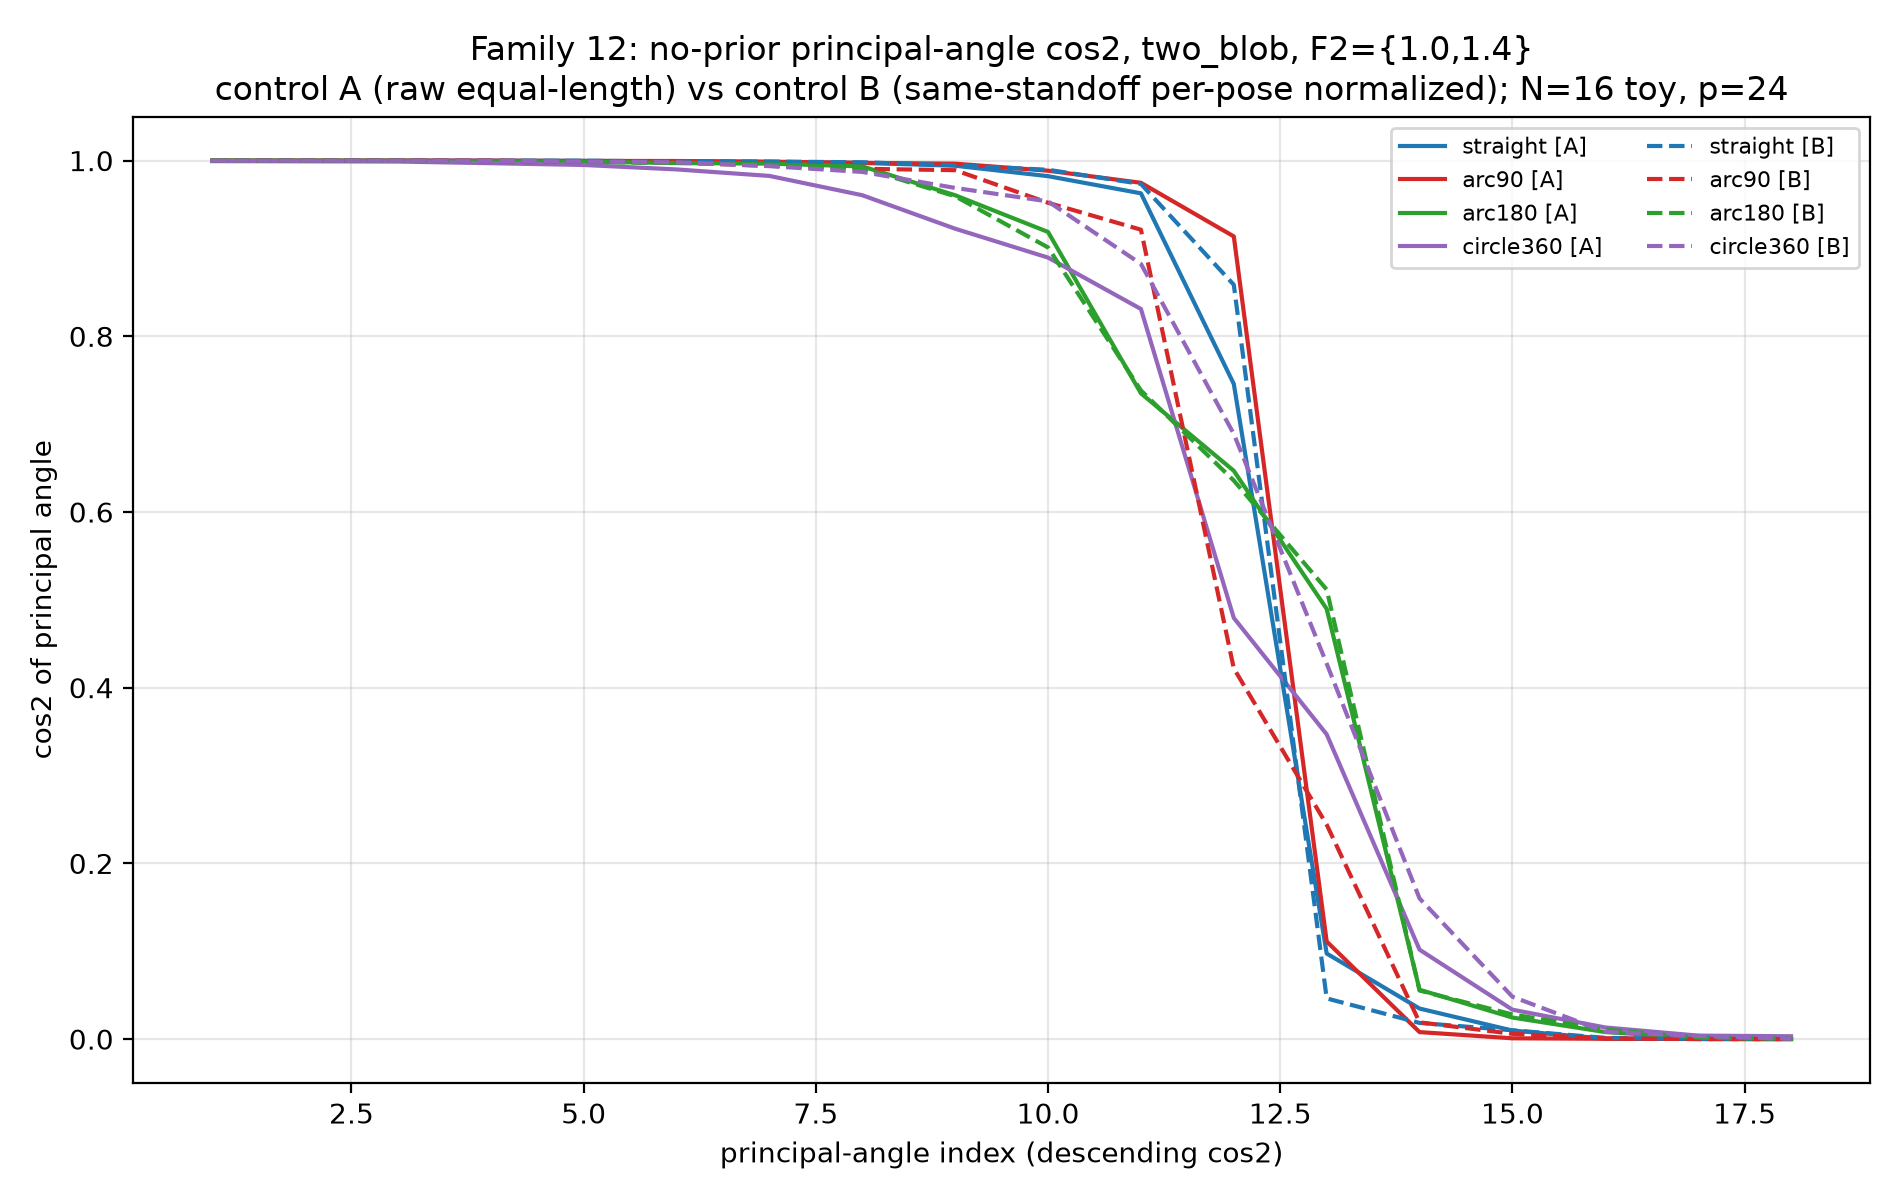
\includegraphics[width=0.86\textwidth]{../figures/family12_principal_angles.png}
\caption{Family 12 no-prior squared-cosine principal-angle curves for the
replicated trajectory cells.}
\label{fig:f12_angles}
\end{figure}

\begin{figure}[htbp]
\centering
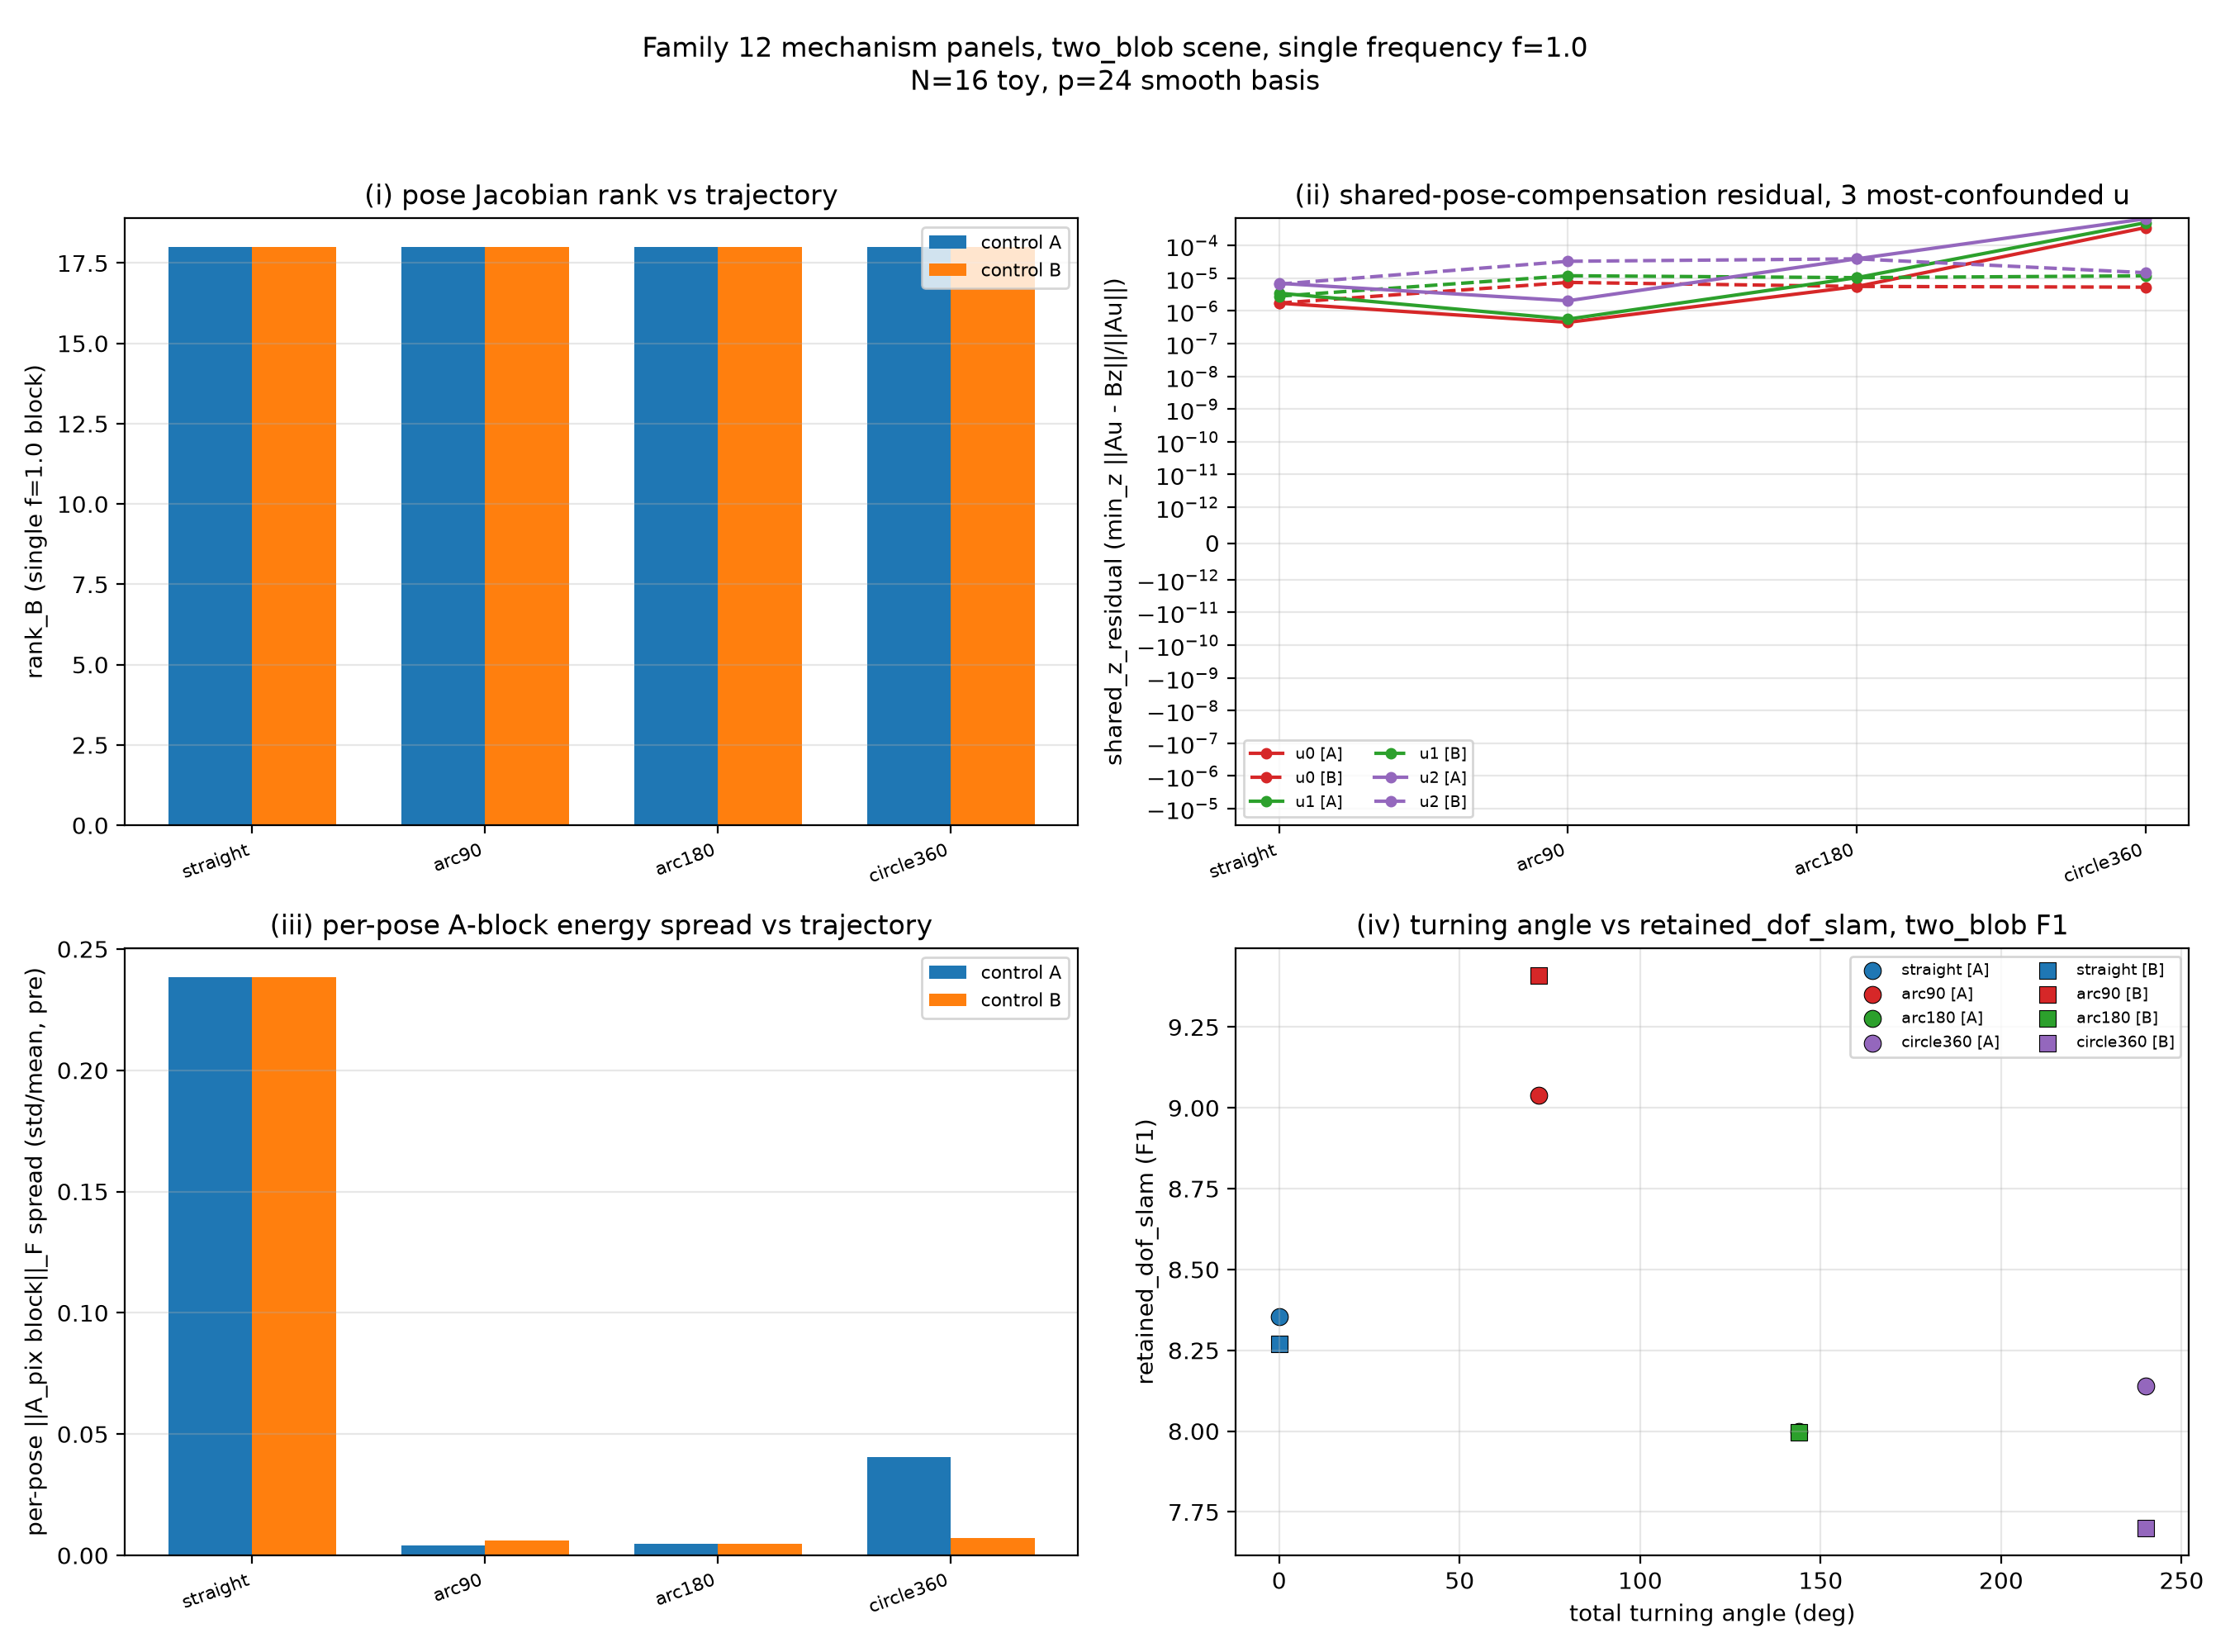
\includegraphics[width=0.86\textwidth]{../figures/family12_mechanism.png}
\caption{Family 12 mechanism diagnostics (shared residuals, per-pose
illumination, geometry).}
\label{fig:f12_mechanism}
\end{figure}

\subsection{Rank-boundary autopsy (Family 13)}\label{sec:family13}

Family 13 (\texttt{results/family13\_rank\_autopsy.json}) autopsies the
Family-9 ring-scene c2 residual of 1
($r_{\mathrm{KIS}}-r_{\mathrm{KSL}}=1$ versus
$r_A+r_B-r_{AB}=0$). The reproduction row matches Family 9 exactly
(ring: $r_A=24$, $r_B=18$, $r_{AB}=42$, $r_{\mathrm{KIS}}=24$,
$r_{\mathrm{KSL}}=23$, residual 1).

\begin{table}[htbp]
\centering
\small
\caption{Family 13 verdict evidence.}
\label{tab:f13}
\begin{tabular}{p{0.36\textwidth} p{0.56\textwidth}}
\toprule
quantity & value (ring; two\_blob reference) \\
\midrule
verdict & (b) tolerance classification of a near-null singular value;
not a discontinuous exact rank change, not unstable subtraction \\
$\sigma_{24}(C)/\sigma_1(C)$ &
$4.74995\times10^{-8}$; $3.90533\times10^{-7}$ \\
$\sigma_{24}(K_{\mathrm{SLAM}})/\sigma_1(K_{\mathrm{SLAM}})$ &
$2.25753\times10^{-15}$; $1.52533\times10^{-13}$ \\
rank of $C$ across predeclared tolerances
$[10^{-16}\ldots10^{-8}]$ & 24 at all nine relative tolerances (both scenes) \\
backward residual $\|K_{\mathrm{SLAM}}-C^TC\|_F$ (rel.\ Fro) &
$5.00069\times10^{-16}$; $3.17762\times10^{-14}$ \\
thin-SVD $1/s^2$ reconstruction residual (rel.\ Fro) &
$1.51994\times10^{-7}$; $8.26455\times10^{-9}$ \\
c2 residual under the Family-2 machine rule &
1; 0 \\
\bottomrule
\end{tabular}
\end{table}

Because $\sigma_{24}(C)/\sigma_1(C)=4.75\times10^{-8}$ squares to
$2.26\times10^{-15}\approx
\sigma_{24}(K_{\mathrm{SLAM}})/\sigma_1(K_{\mathrm{SLAM}})$, the directly
formed $K_{\mathrm{SLAM}}=A^TPA$ drops one near-null mode under the machine
rank rule while the factorized $C=(I-ZZ^T)A$ stays full rank; $C$ remains full
rank at every one of the nine predeclared relative tolerances
($10^{-16}$--$10^{-8}$), and $K_{\mathrm{SLAM}}$ agrees with $C^TC$ at
machine-level relative Frobenius error ($5.0\times10^{-16}$). The thin-SVD
reconstruction residual ($1.5\times10^{-7}$) is the larger roundoff floor
caused by scaling $K_{\mathrm{SLAM}}$ by $1/s^2$. The verdict is tolerance
classification, supported by the computed finite-dimensional numbers; no
theorem is claimed.

\paragraph{Engineered algebraic falsifier.}
The Family-5 parent generalized-derivative construction
$B(t)=U\,\mathrm{diag}(s_1,\ldots,s_{17},|t|s_{18})V^T$ is reused read-only
as an algebraic control: $\mathrm{rank}(B)$ drops 18$\to$17 at $t=0$, the
no-prior projector jumps by operator norm 1.0, retained mass jumps from
$9.40716$ (every $t>0$) to $10.40528$ ($t=0$), and the relative Frobenius
information jump is $0.13996$. This falsifier is explicitly labeled an
algebraic control, not a physical event, and it demonstrates where
constant-rank derivative formulas become inapplicable (see
Section~\ref{sec:family14}).

\begin{figure}[htbp]
\centering
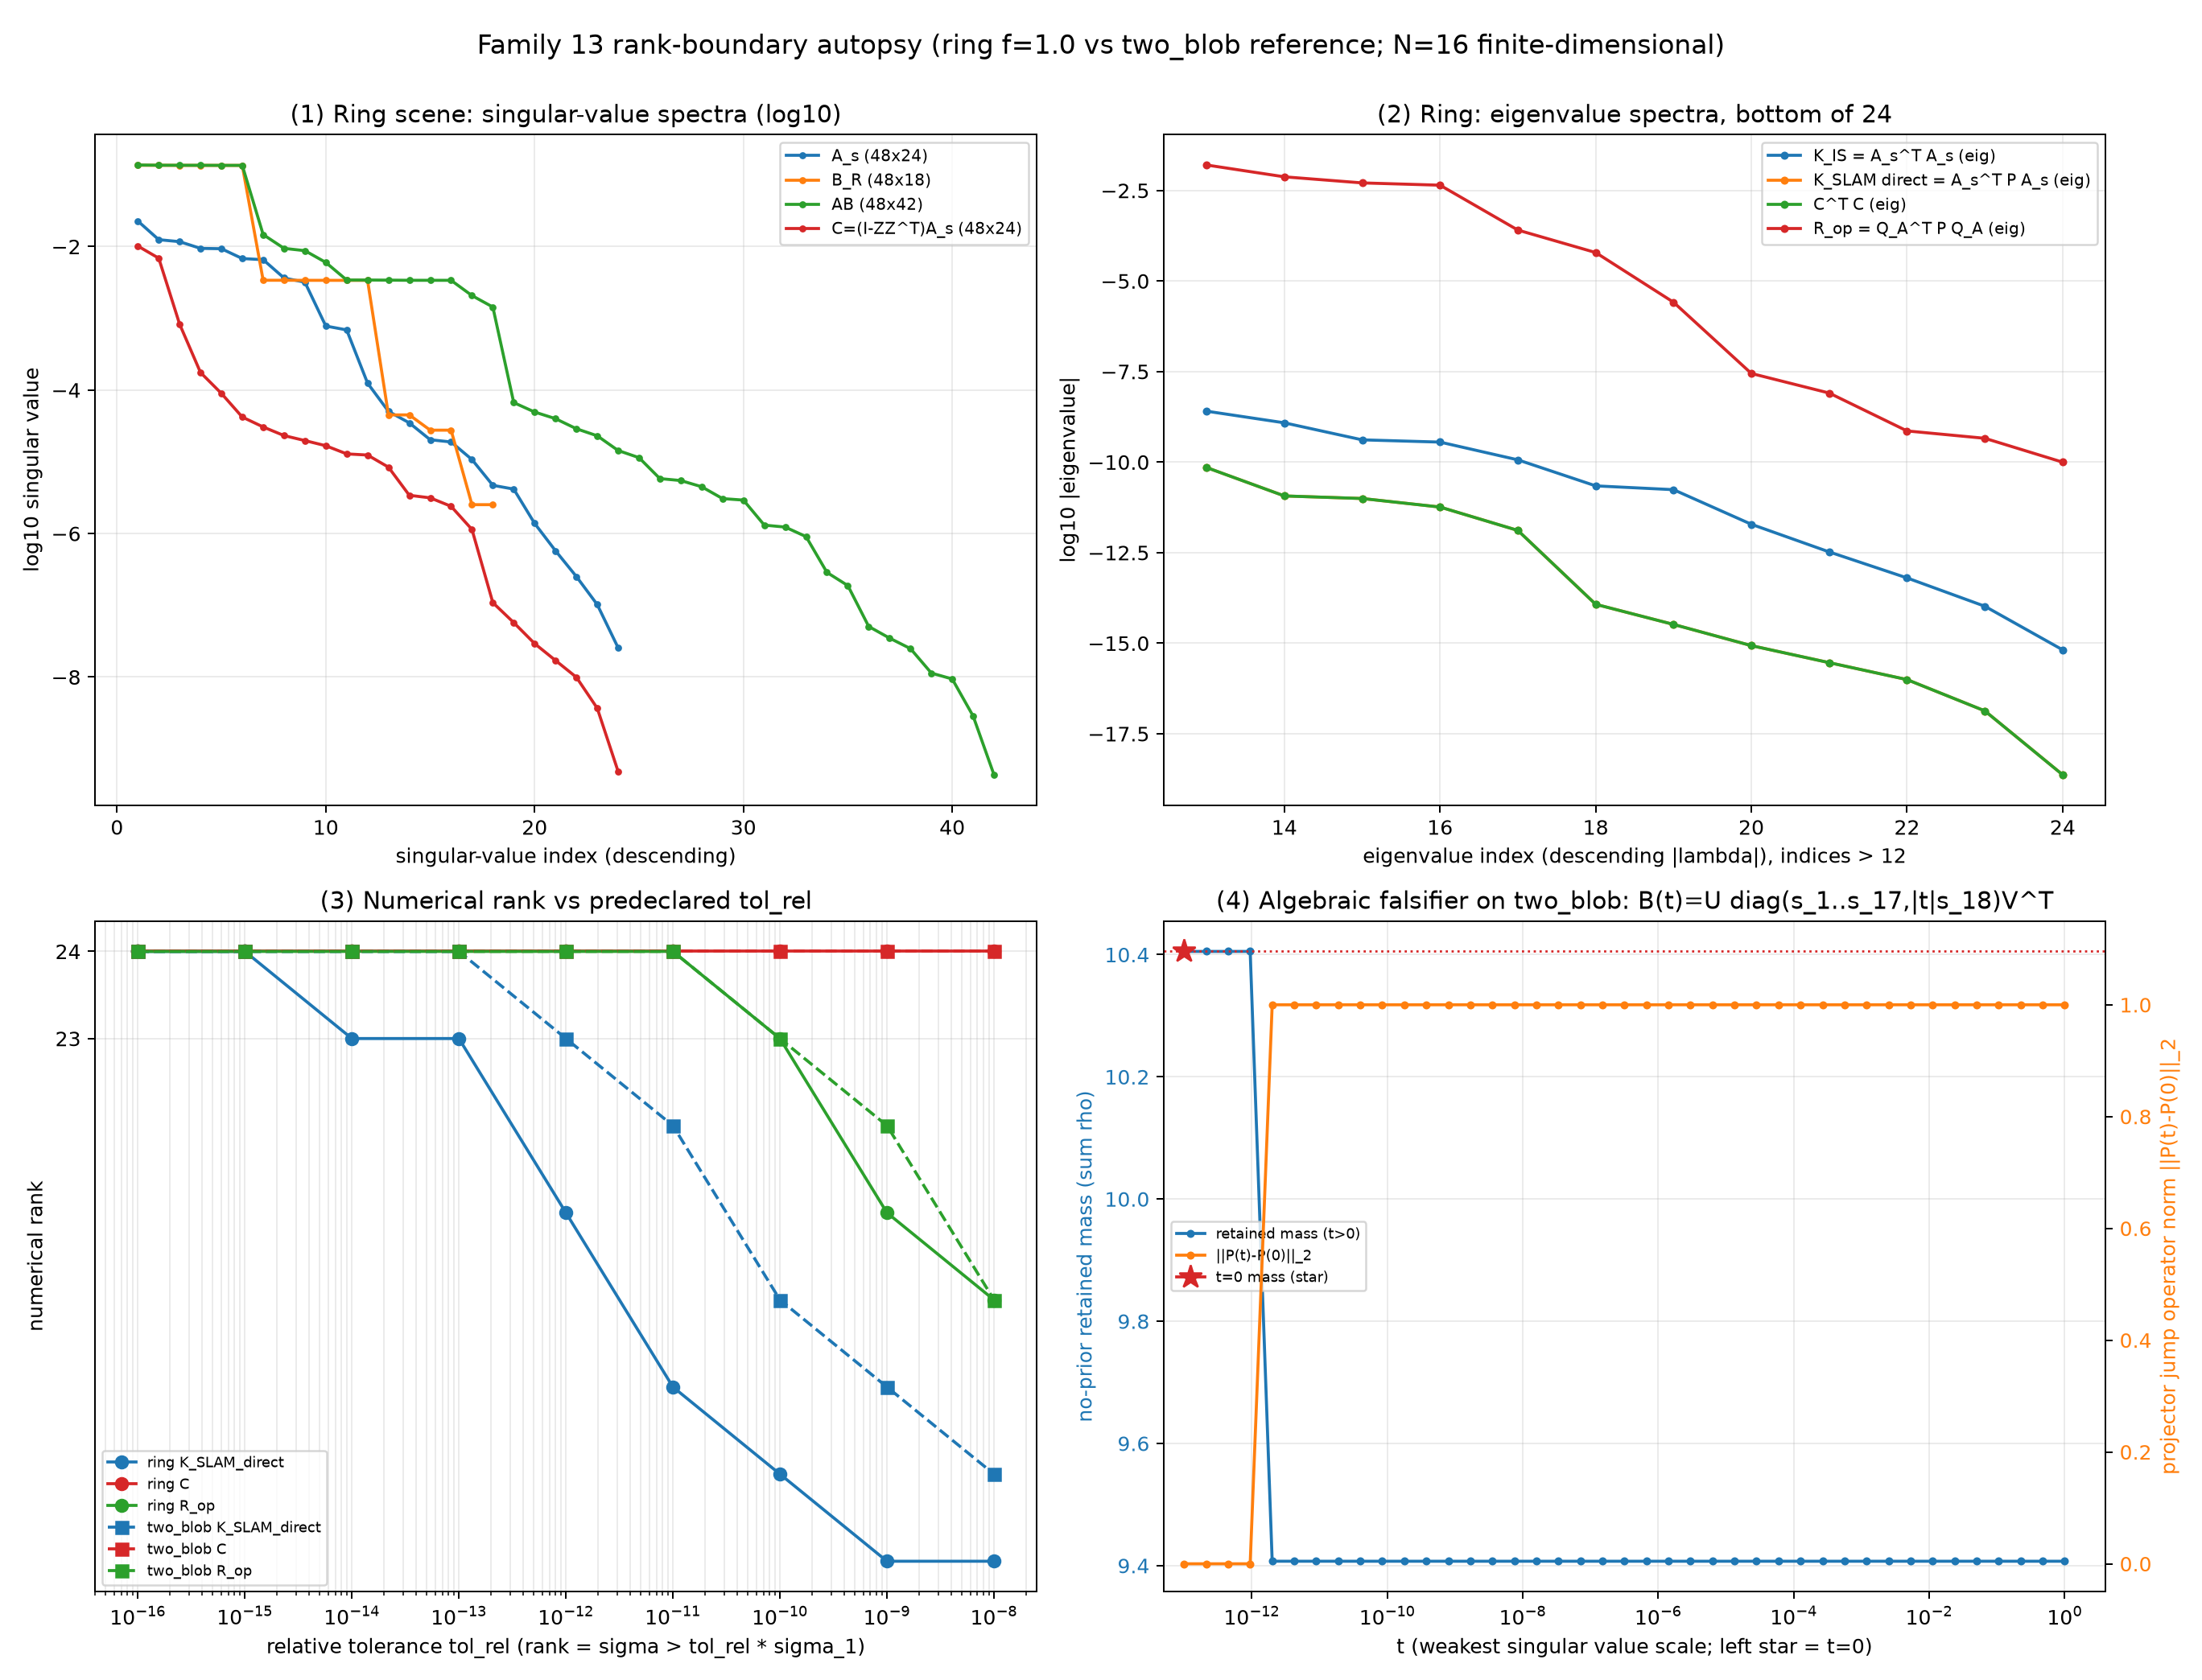
\includegraphics[width=0.86\textwidth]{../figures/family13_rank_autopsy.png}
\caption{Family 13 ring-scene rank autopsy: spectra, tolerance grid, and
falsifier.}
\label{fig:f13}
\end{figure}

\subsection{Robustness scope and demotion (Family 14)}\label{sec:family14}

Family 14 (\texttt{results/family14\_robustness\_scope.json}) audits the scope
of the stored robustness evidence without running a new Helmholtz operator.
Its recomputation of the affine tangent certificate from the Family 5b2
ingredients reproduces every stored row exactly at IEEE double precision
(max abs relative difference 0.0): $L_{\mathrm{cert,affine}}=
1.1309\times10^{-2}$, $1.1438\times10^{-2}$, $1.1895\times10^{-2}$ at
$\epsilon=10^{-3}$, $3\times10^{-3}$, $10^{-2}$.

\begin{table}[htbp]
\centering
\small
\caption{Family 14 scope-audit numbers at $\epsilon=10^{-2}$ unless noted.}
\label{tab:f14}
\begin{tabular}{p{0.36\textwidth} p{0.56\textwidth}}
\toprule
quantity & value \\
\midrule
recomputed affine certificate (eps $10^{-3}$/$3\times10^{-3}$/$10^{-2}$) &
$1.130863\times10^{-2}$ / $1.143821\times10^{-2}$ /
$1.189479\times10^{-2}$; rel.\ diff to stored = 0 \\
FD Jacobian validation (global rel.\ Fro) &
J$_A$ $5.990607\times10^{-7}$; J$_B$ $5.374392\times10^{-7}$ \\
full nonlinear worst sampled quotient (500 dirs, seed 9191, eps=$10^{-2}$) &
$3.228342\times10^{-4}$ \\
$L_{\mathrm{cert,affine}}$ at eps=$10^{-2}$ &
$1.189479\times10^{-2}$ \\
margin / ratio (full nonlinear at eps=$10^{-2}$) &
$1.157196\times10^{-2}$ / 36.84 \\
affine worst sampled quotient (2000 dirs, seed 7171, eps=$10^{-2}$) &
$3.744008\times10^{-4}$; margin $1.152039\times10^{-2}$; ratio 31.77 \\
generalized-derivative factored backward residuals &
$4.040062\times10^{-16}$ (finite prior) /
$9.238499\times10^{-16}$ (no prior) \\
generalized-derivative prediction slopes & $\sim2$
(2.0017/2.0015/1.9998 finite prior; 2.0041/1.9958/1.9924 no prior) \\
repeated-eigenvalue cluster control &
six structural $\rho=1$ modes stay at one to $\le1.443290\times10^{-15}$;
compressed-derivative spectral norm $2.297307\times10^{-10}$ \\
\bottomrule
\end{tabular}
\end{table}

\begin{quote}
All full nonlinear execution-error robustness claims are DEMOTED to
empirical/structural observations; only the affine tangent certificate is
retained as a finite-dimensional conditional certificate.
\end{quote}

The demotion is explicit and recorded verbatim in the Family 14 JSON.
Consequently, no interval proof is claimed, no
Hankel bound is claimed, no continuum robustness is claimed, and no certified
robustness for the full nonlinear model is claimed. The generalized-derivative
formulas were validated on simple positive-gap modes (factored backward
residuals $4.0\times10^{-16}$/ $9.2\times10^{-16}$ with prediction slopes
$\sim2$) and require locally constant rank, so they are inapplicable at rank
events; repeated generalized eigenvalues require compressed derivatives, for
which only cluster-control evidence exists (six $\rho=1$ modes at one to
$\le1.44\times10^{-15}$; compressed derivative norm $2.30\times10^{-10}$).
Zero sampled violations over 500 or 2000 directions at the tested $\epsilon$
are reported as observed evidence, not certification.

\subsection{Mixed-tangent Born isolation control (Family 15)}\label{sec:family15}

Family 15 (\texttt{results/family15\_born\_control.json}) compares the Born
map tangent with the full-wave map tangent in the smooth $p=24$ coefficient
space over $s\in\{0.001,0.01,0.03,0.1,0.3,1.0\}$. It deliberately applies the
same full-wave pose block $B_{\mathrm{full}}(s)$ to both map tangents. Thus its
Schur and no-prior rows use $(A_{\mathrm{Born}},B_{\mathrm{full}})$ and are a
\emph{mixed-tangent isolation control}, not a complete Born-SLAM Fisher model.
The composition identity
$A_{\mathrm{Born}}=G_S\,\mathrm{diag}(E^{\mathrm{inc}})$ is verified against an
explicit blockwise stack at every scale with residual 0.0 (a bitwise-identical
code path); the independent Family-3b zero-background check has relative
Frobenius residual $7.05\times10^{-17}$.

\begin{table}[htbp]
\centering
\small
\caption{Family 15 mixed-tangent control; all Schur quantities in this table
share $B_{\mathrm{full}}$.}
\label{tab:f15}
\begin{tabular}{p{0.36\textwidth} p{0.56\textwidth}}
\toprule
quantity & value \\
\midrule
Born composition identity & rel.\ Fro 0.0 at all six scales \\
observed log-log slopes & $A$: 1.0026; $K_{\mathrm{IS}}$: 0.9944;
mixed $K_{\mathrm{eff}}$: 0.9942 ($r^2\ge0.9998$) \\
relative errors at $s=0.1$ & $A$: 5.05\%; $K_{\mathrm{IS}}$/mixed
$K_{\mathrm{eff}}$: 7.10\% \\
relative errors at $s=1$ & $A$: 50.5\%; $K_{\mathrm{IS}}$/mixed
$K_{\mathrm{eff}}$: approximately 65.2\% \\
principal angles between the two three-dimensional most-confounded
coefficient subspaces & $9.72\times10^{-4}$/$1.81\times10^{-2}$/$4.49\times
10^{-2}$ deg at $s=0.001$; $0.971$/$15.325$/$64.860$ deg at $s=1$ \\
\bottomrule
\end{tabular}
\end{table}

\paragraph{Literature control and statistical caveat.}
Diong et al.~\cite{diong} study the mean, variance, and estimation error of a
Born-based maximum-likelihood estimator relative to an exact-model
Cram\'er--Rao bound. In a correctly specified linear Gaussian model,
$A_{\mathrm{Born}}^TA_{\mathrm{Born}}$ is an information matrix; identifying
its inverse with an estimator covariance additionally requires the relevant
full-rank and unbiasedness conditions. Our mixed $K_{\mathrm{eff}}$ is a local
pose-prior information comparison, not an estimator-MSE reproduction. The
published geometry, normalization, noise model, parameterization, and units
were not reproduced, so Family 15 is neither an external benchmark nor a
numerical match to that paper.

\begin{figure}[htbp]
\centering
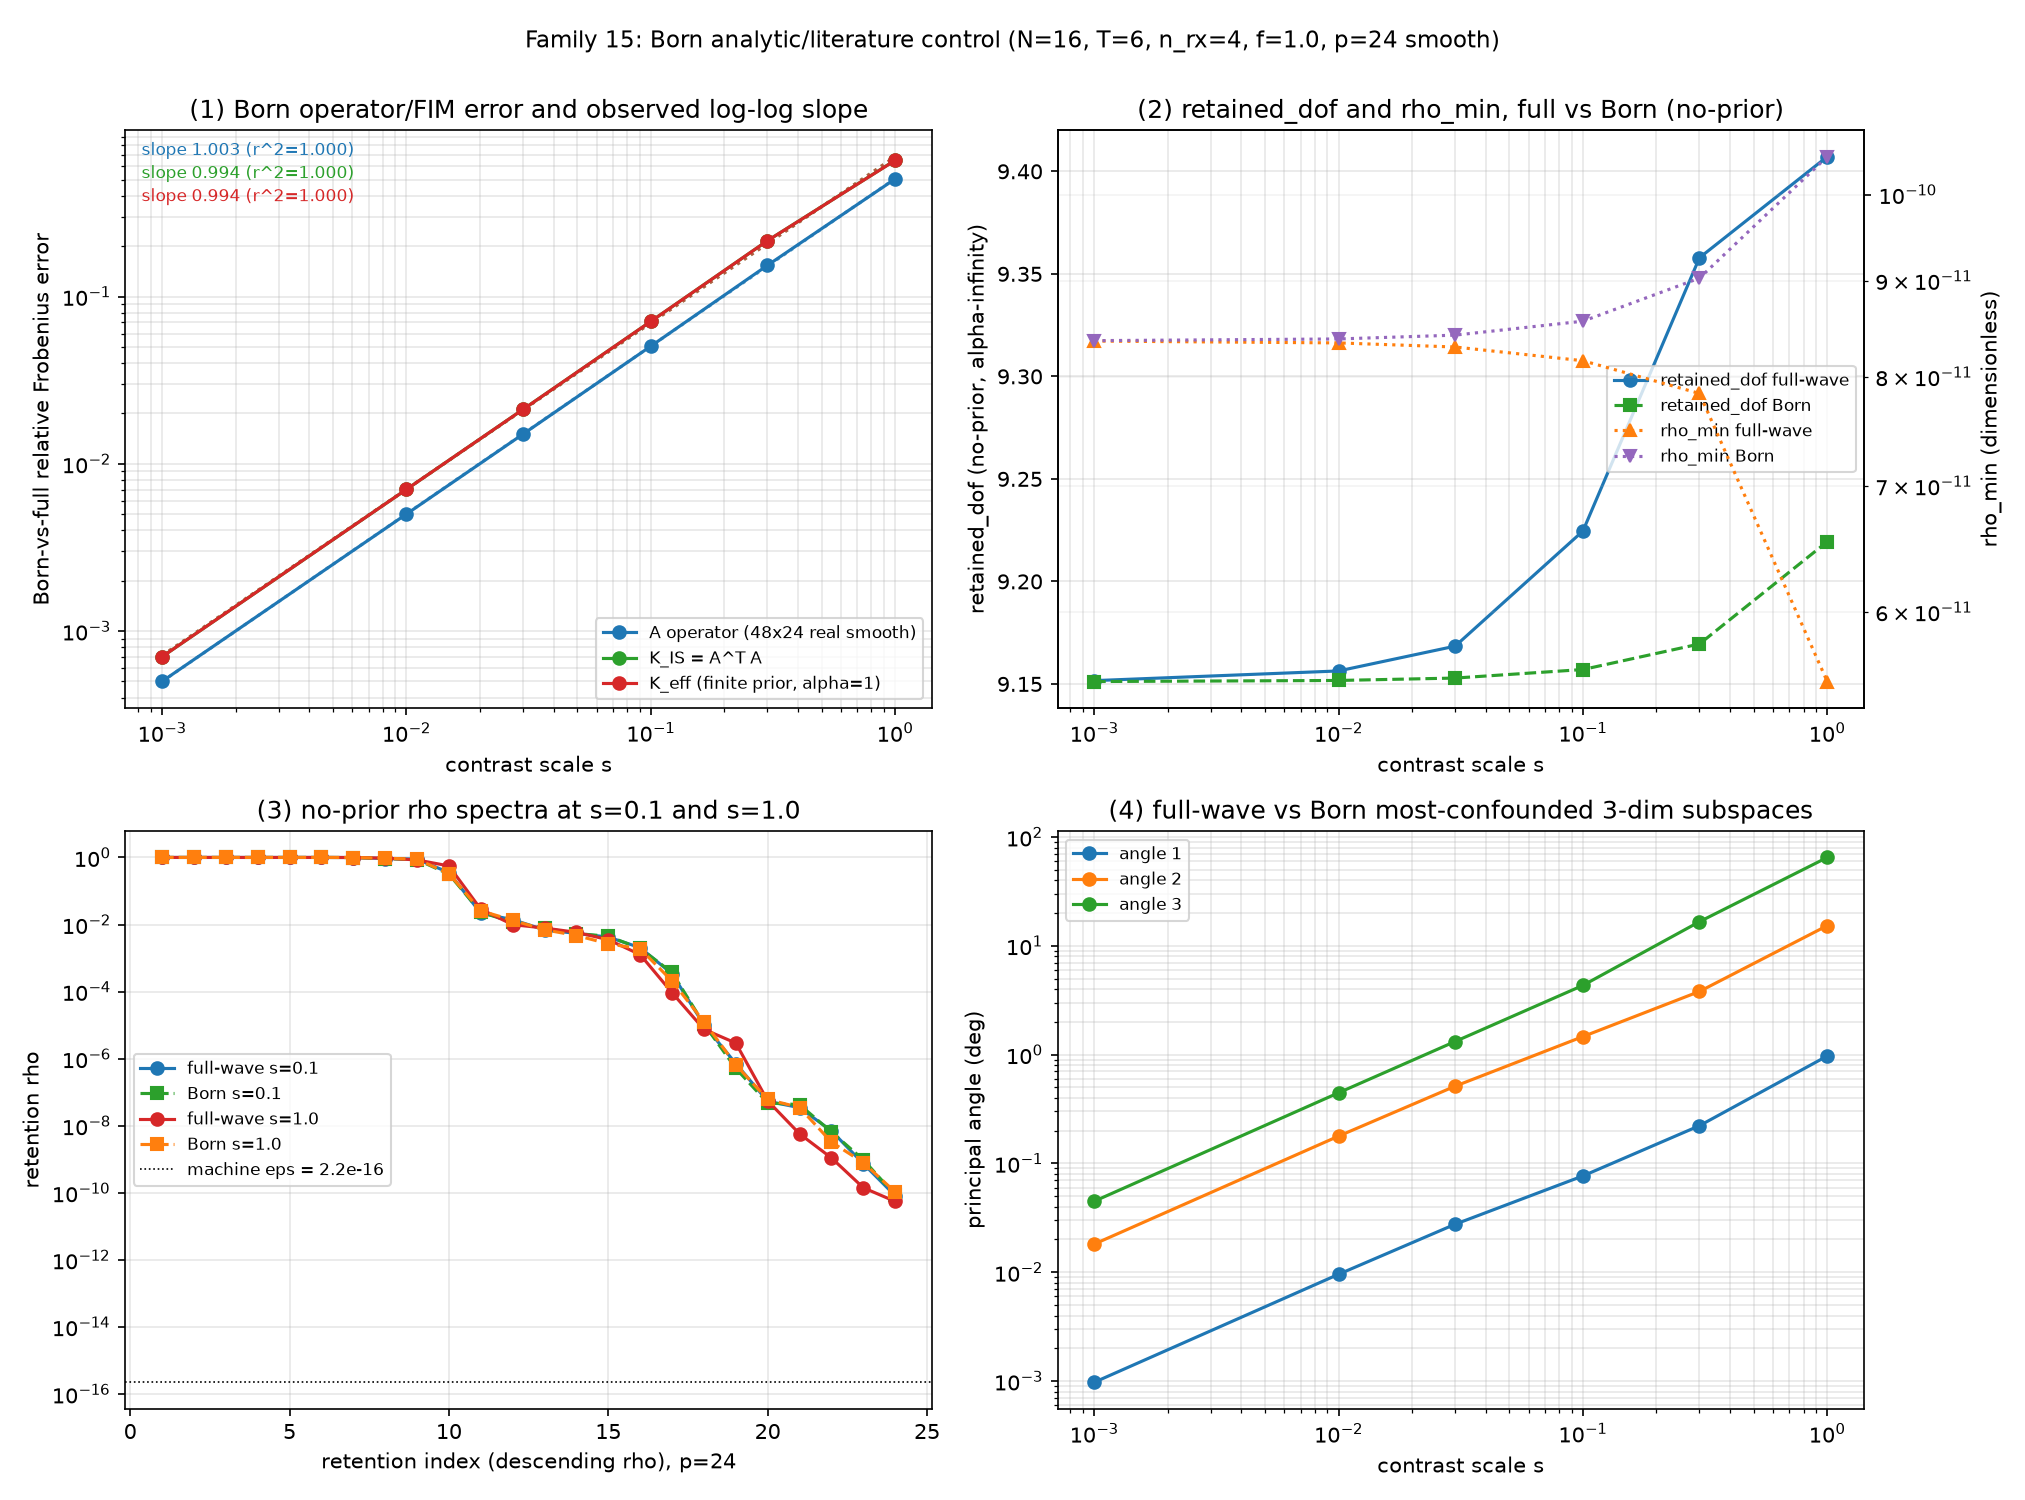
\includegraphics[width=0.86\textwidth]{../figures/family15_born_control.png}
\caption{Family 15 mixed-tangent Born/full-wave relative errors, slopes, and
most-confounded coefficient-subspace separation.}
\label{fig:f15}
\end{figure}

\subsection{Complete Born pose tangent and rank-stratum limit (Family 15b)}
\label{sec:family15b}

Family 15b (\texttt{results/family15b\_born\_pose\_control.json}) closes the
semantic gap above by constructing the actual Born pose Jacobian. For pose
$t$ and coordinate $\ell$, the implemented discrete derivative is
\[
[B_B]_{t,\ell}=(D_{X_\ell}G_{S,t})(\chi\odot E_t^{\mathrm{inc}})
 +G_{S,t}(\chi\odot D_{X_\ell}E_t^{\mathrm{inc}}).
\]
At $s=0.1$, centered differences over all 18 pose coordinates have relative
Frobenius errors $1.75666\times10^{-5}$, $1.58100\times10^{-6}$, and
$1.75667\times10^{-7}$ at steps $10^{-3}$, $3\times10^{-4}$, and $10^{-4}$,
respectively. The fitted slope is 1.999997 ($r^2$ within $3\times10^{-13}$ of
one), numerically supporting the analytic discrete derivative.

\paragraph{Proposition (finite-dimensional Born scaling).}
Let $F_B(\chi,X)=A_0(X)\chi$ and set $\chi=s\bar\chi$. Define
$B_1=D_X[A_0(X)\bar\chi]$. Then
\[
A_B(s)=A_0,\qquad B_B(s)=sB_1.
\]
For every $s\ne0$, $\mathrm{Range}(B_B(s))=\mathrm{Range}(B_1)$, so the
no-prior projector and $K_{\mathrm{SLAM}}$ are independent of $|s|$. At
$s=0$, $B_B(0)=0$ and $K_{\mathrm{SLAM}}(0)=K_{\mathrm{IS}}$. Hence the
no-prior endpoint is discontinuous unless
$\mathrm{Range}(A_0)\perp\mathrm{Range}(B_1)$. With $J_X=\alpha I$ and
$\alpha>0$, the finite-prior loss satisfies
\[
L_s=A_0^T(sB_1)(s^2B_1^TB_1+\alpha I)^{-1}(sB_1)^TA_0,
\qquad
\|L_s\|_2\le \frac{s^2}{\alpha}\|A_0^TB_1\|_2^2.
\]
\emph{Proof.} Differentiating the bilinear Born map gives the two tangent
identities. Nonzero scalar multiplication preserves a range and its orthogonal
projector. At $s=0$ the pose tangent is zero. Finally,
$(s^2B_1^TB_1+\alpha I)^{-1}\preceq\alpha^{-1}I$ gives the stated norm bound.
The bound does not cover a semidefinite pose prior, whose range and kernel must
be treated separately. \hfill$\square$

\begin{table}[htbp]
\centering
\small
\caption{Family 15b complete-pair checks and rank-stratum evidence.}
\label{tab:f15b}
\begin{tabular}{p{0.38\textwidth} p{0.54\textwidth}}
\toprule
quantity & value \\
\midrule
maximum scale residuals & $A_B$: 0;
$B_B(s)/s$: $5.53\times10^{-16}$; nonzero-$s$ projector:
$4.52\times10^{-14}$ \\
finite-prior bound & all six tested rows satisfy the bound \\
complete-Born no-prior retained DOF & 9.151114708 at $s=0.001$ and $s=1$;
24.000000000 at $s=0$ \\
observed full-versus-Born slopes & $A$: 1.003; $B$: 1.001;
$K_{\mathrm{IS}}$: 0.994; complete $K_{\mathrm{eff}}$: 0.994;
$K_{\mathrm{SLAM}}$: 0.982; projector gap: 1.008 \\
complete-pair errors at $s=0.1$ & $A$: 5.05\%; $B$: 1.77\%;
$K_{\mathrm{eff}}$: 7.10\%; pose-projector gap: 1.67\% \\
complete-pair errors at $s=1$ & $A$: 50.5\%; $B$: 17.8\%;
$K_{\mathrm{eff}}$: 65.2\%; pose-projector gap: 17.8\% \\
\bottomrule
\end{tabular}
\end{table}

The constant nonzero-$s$ no-prior retained DOF is a normalized range effect:
it does not imply that an arbitrarily weak scatterer carries finite practical
pose information. Indeed $\|B_B(s)\|=O(|s|)$, while the no-prior projector
discards magnitude. The positive-prior $O(s^2)$ result restores the physically
relevant vanishing-information scale. This distinction is the main
weak-scattering semantic correction supplied by Family 15b.

\begin{figure}[htbp]
\centering
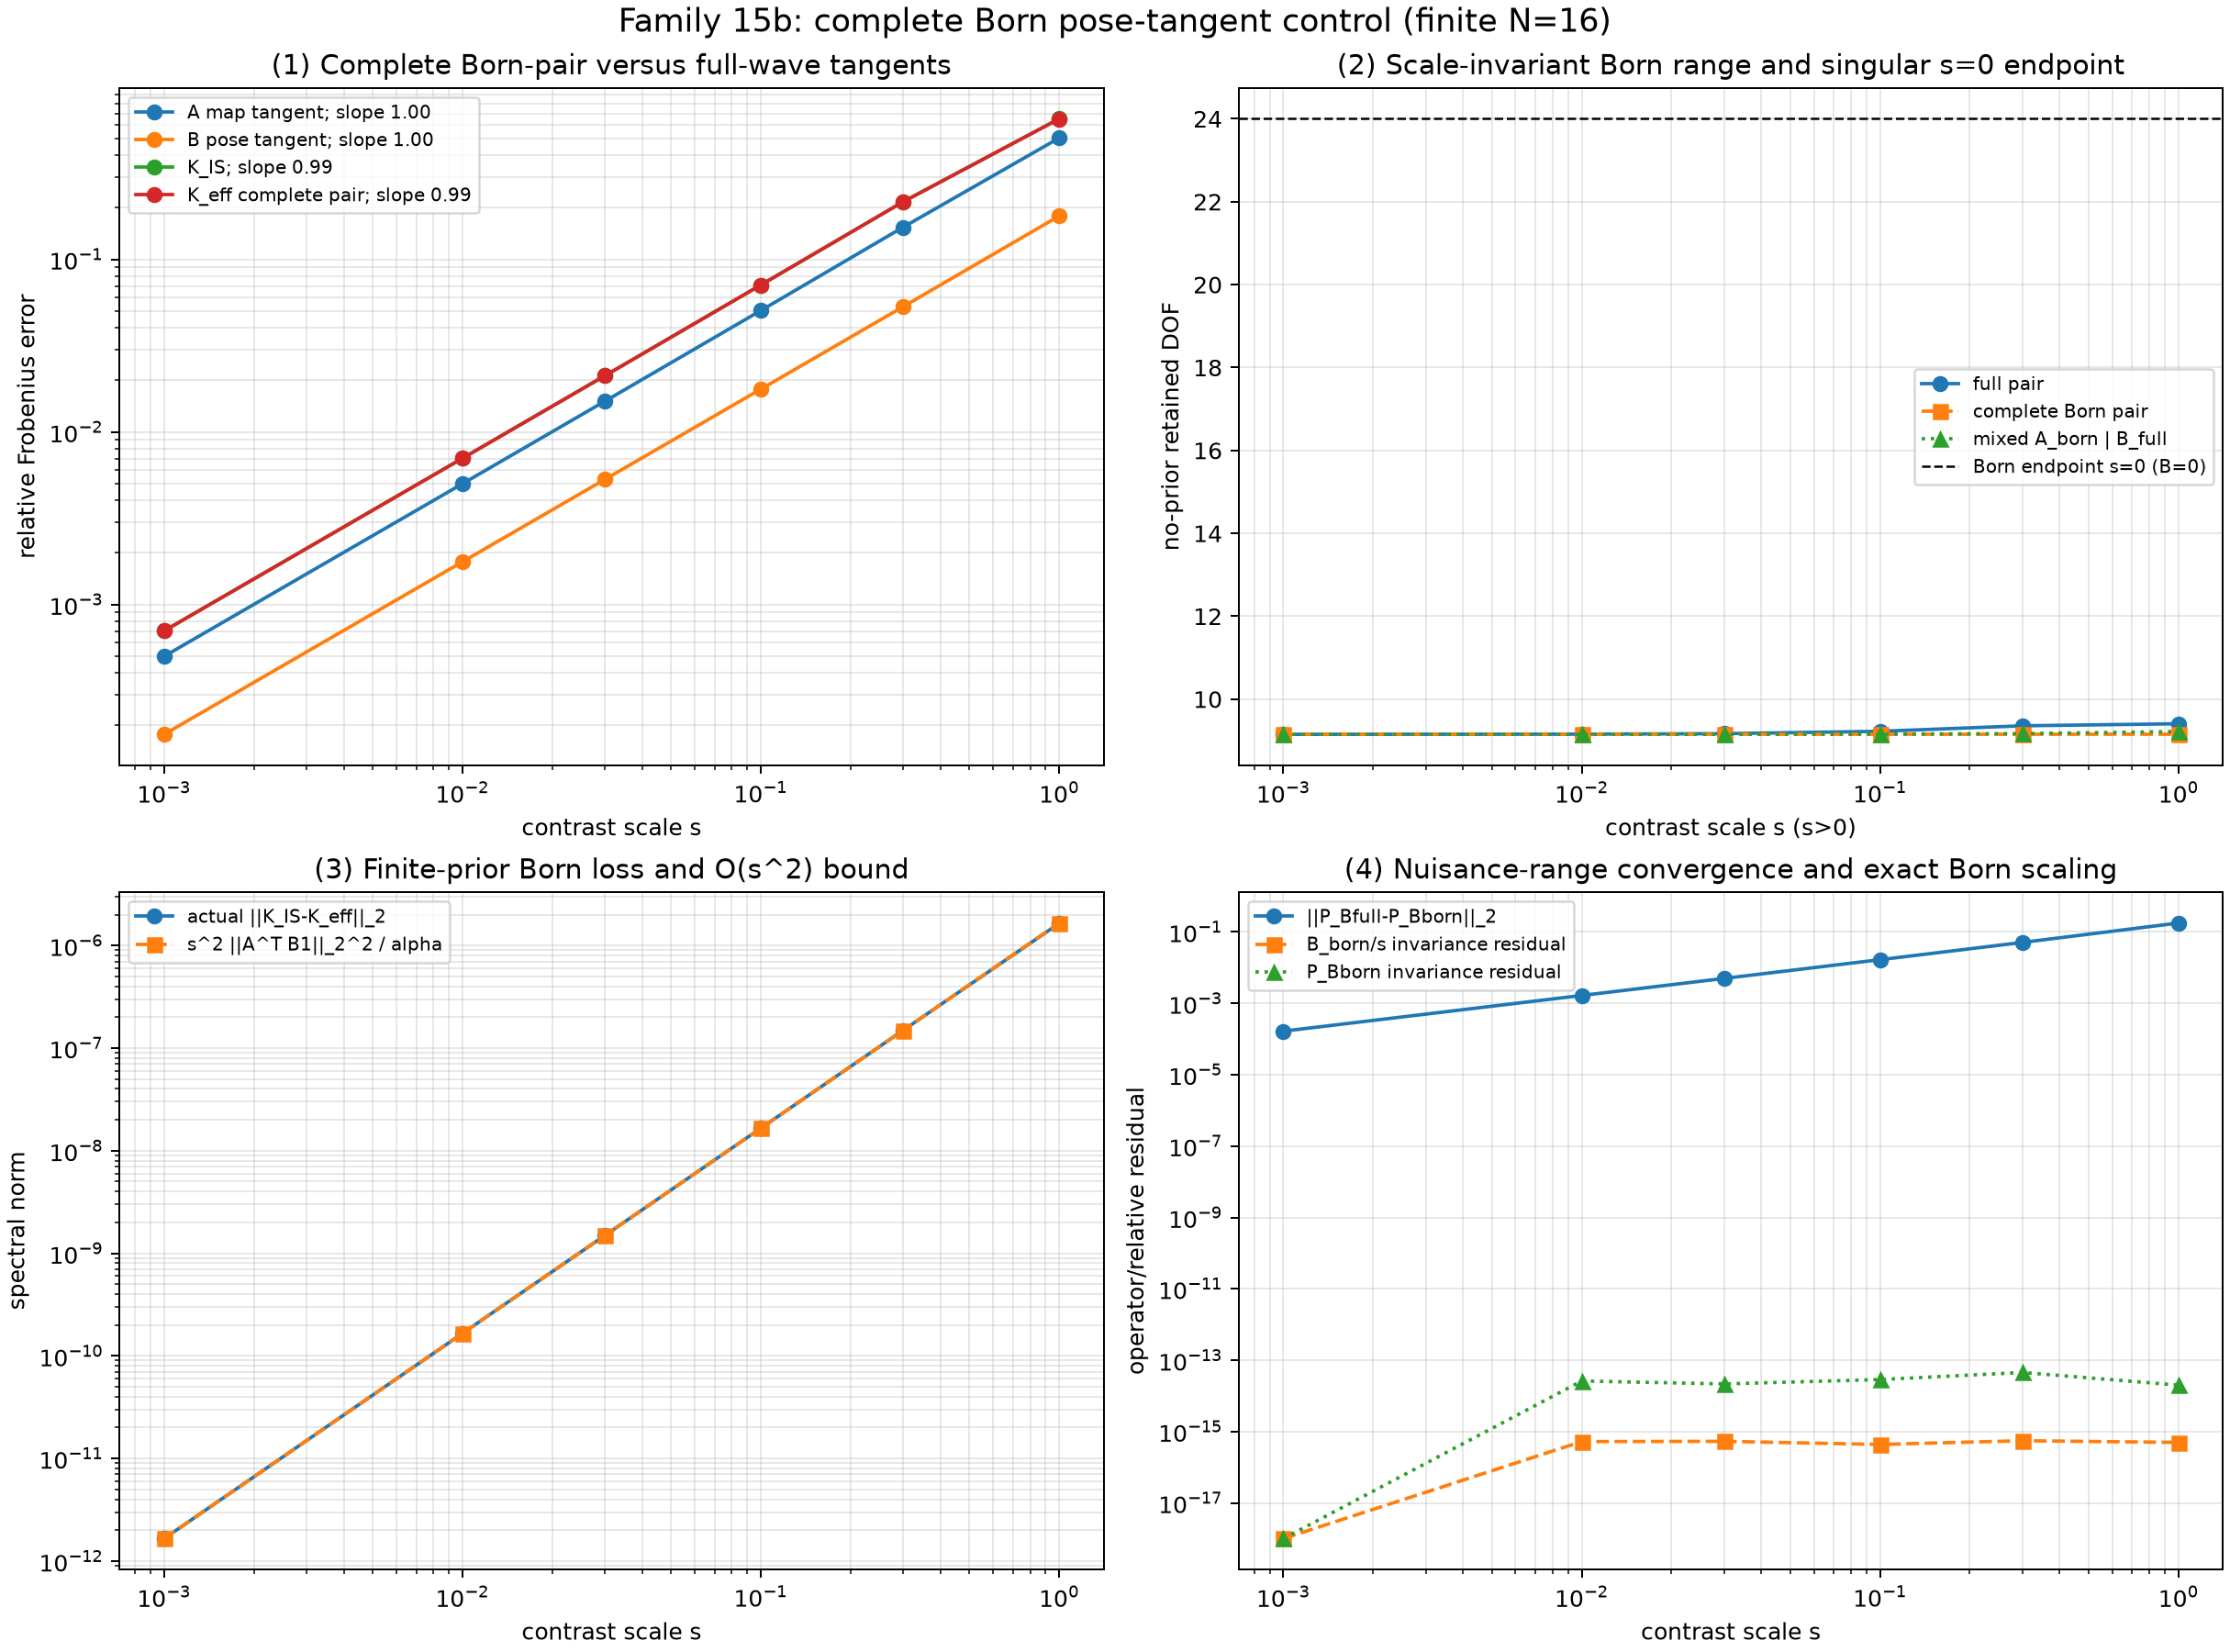
\includegraphics[width=0.86\textwidth]{../figures/family15b_born_pose_control.png}
\caption{Family 15b analytic pose-derivative check, complete-pair deviations,
nonzero-scale projector invariance, and the singular $s=0$ endpoint.}
\label{fig:f15b}
\end{figure}

\section{Related work}\label{sec:related}

The ingredients combined here are mature; none is introduced as new in
isolation. Schur and pseudoinverse elimination of nuisance parameters appears
throughout self-calibration and bilinear inverse problems
\cite{ling,libresler}. Radar autofocus supplies a particularly close physical
antecedent: antenna-position errors can be represented as image-domain shift
kernels in sparse blind deconvolution~\cite{mansour}, while joint SAR imaging
and motion-induced phase correction has been treated by alternating or joint
optimization~\cite{onhon,scarnati}. Those works estimate image and calibration
or phase variables, but do not use the full-wave volumetric contrast tangent
and shared physical SE(2) pose parameterization studied here.

The closest retrieved map--pose information neighbor is the posterior
Cram\'er--Rao analysis of distributed-MIMO radio SLAM by Deutschmann et
al.~\cite{deutschmann}, whose map consists of parametric specular surfaces.
Jacobian/Fisher-rank observability has also yielded necessary and sufficient
conditions for SLAM-based TDOA array calibration~\cite{su}. Most directly,
Karthik and Ghosh jointly reconstruct inverse-scattering contrast and localize
transmitters~\cite{karthik}; therefore joint inverse scattering and localization
itself is not a novelty claim of this draft. The accessible metadata for these
neighbors does not establish the present whitened/realified volumetric
map-tangent versus pose-tangent retention construction, but full-text coverage
was incomplete and absence of that formula cannot be inferred.

For inverse scattering, multifrequency stability and reconstruction are
established themes~\cite{entekhabi,shea,weidling}. The subspace-based
optimization method (SOM) uses the singular structure of the
current-to-scattered-field operator~\cite{chen}; Section~\ref{sec:family8}
keeps that current-space spectrum distinct from the map-tangent spectrum used
here. Sensor/frequency selection under the Born approximation has likewise
been posed as singular-value optimization~\cite{capozzoli}, so the trajectory
experiments here are interpreted as falsifiers of particular ordering rules,
not as the invention of spectral acquisition design. Radar SLAM studies
provide the engineering context~\cite{burnett,hilger}, but the present runs do
not reproduce their sensors or datasets.

For the Born comparison, Diong et al.~\cite{diong} analyze the mean, variance,
and error of a Born-based estimator relative to an exact-model Cram\'er--Rao
bound. Family 15 is only a mixed-tangent internal control; Family 15b supplies
the complete Born pose tangent and an exact rank-stratum proposition. Neither
family reproduces the published estimator, bias, geometry, normalization,
noise model, parameterization, units, or numerical values, so neither is an
external validation.

The synthesis boundary is therefore precise: nuisance elimination, principal
angles, gauge analysis, bilinear identifiability, multifrequency stability,
joint reconstruction/localization, and radar SLAM all have prior art. The
tested contribution of this draft is the explicit finite-dimensional
pose-confounding retention construction for whitened/realified nonlinear
full-wave volumetric contrast tangents, its executable falsifiers, and the
complete-Born rank-stratum limit. This draft makes no priority claim; the
novelty boundary is retrieval-bounded, and the 429-limited search is a
retrieval limitation, not a novelty verdict.

\section{Limitations and open questions}\label{sec:limits}

All executed claims are finite-dimensional. The following therefore remain
open:
\begin{itemize}
\item \emph{Continuum transfer and stable transversality.} The finite
discrete identities do not prove closed-range properties,
$\inf_{Au\ne0}\mathrm{dist}(Au,\mathrm{Range}(B))/\|Au\|>0$, or convergence of
the retention spectrum under discretization. Family 7 refinement is a
finite-grid diagnostic only: the decreasing $\theta_{\min}$ trend and the
constant near-confounded count are observed on N=16..48, with no continuum
convergence or stable-transversality theorem. \OPN{}
\item \emph{Rank events and transversality.} No rank event occurred along the
Family 5 random path or the Family 7 frequency sweep; the 21 literal
near-crossing flags sit in the lowest numerical near-null pairs of
$K_{\mathrm{eff}}$ and are not certified crossings. Continuity/rank-event
theory for the retention spectrum near gap closure remains open, and only
cluster/projector treatments are admissible there. \OPN{}
\item \emph{Global nonlinearity and cycle skipping.} The local tangent/Fisher
formulation does not address cycle skipping, phase wrapping, wrong data
association, posterior multimodality, or basins of attraction. \OPN{}
\item \emph{Colored-noise realism.} Family 6 declares a synthetic covariance
$C_f=\sigma_f^2(I_T\otimes R_{\mathrm{rx}})$ with a Mat\'ern-1/2 receiver
factor and per-frequency SNR normalization; the whitening and algebraic
checks pass under that declared model only. Physical realism, measured noise
covariance, and estimator-level correlated-noise behaviour are not
established. \OPN{}
\item \emph{Trajectory normalization and standoff.} Family 4c per-pose
$A$-block normalization is a declared gain control, not a physical noise
covariance or an optimal-SNR whitening rule. Same standoff fixes curved-path
range but changes design/polyline length with angular coverage, and the
straight path still varies standoff, so no universal trajectory-ordering
theorem is asserted. \OPN{}
\item \emph{SOM/current-space distinction.} Family 8 checks, on the tested
finite scenario, that the current-space $G_S$ composition and range
containment hold while the $V_{GS}$/SOM and map-tangent $V_A$/$K_{\mathrm{eff}}$
mode subspaces are distinct. This is numerical evidence, not a continuum
theorem, and no pullback/composition theorem $A=G_ST_\chi$ or SOM quality
claim was proved. \OPN{}
\item \emph{Interval Lipschitz certification.} Formal interval certification of
the full nonlinear operator-Lipschitz constant remains open. The Family 5b2
affine tangent certificate is rigorous for the affine model only and remains
conditional on the numerically computed finite-difference Jacobians; the
full-model result is a derived structural bound with a sampled ingredient
envelope, not a formal interval certificate. Round 3 makes the demotion
explicit (Section~\ref{sec:family14}): all full nonlinear execution-error
robustness claims are empirical/structural observations, with only the affine
tangent certificate retained as a finite-dimensional conditional certificate.
No interval/uniform nonlinear certificate, no Hankel bound, and no continuum
robustness are claimed. \OPN{}
\item \emph{Nonlinear free-pose covariance in the NLS toy.} Family 10 shows
that on the tested 120-trial scheme the linearized free-pose covariance does
not match the empirical fixed-pose sandwich covariance, with large sampling
variance in the most-confounded directions. The finite-dimensional toy is not
an online SLAM system, and no estimator-level or real-system covariance theory
is asserted. \OPN{}
\item \emph{Scene-specific frequency-diversity exception.} Family 11
replicates the non-monotone peak and high-SNR plateau in 12/12 directions for
two\_blob and ring at f2=1.4/1.8, but low\_contrast/f2=1.8 replicates only
2/3 directions (u1 lacks an interior peak). Frequency diversity is finite
dimensional and scene specific; no universal frequency-design rule is claimed.
\OPN{}
\item \emph{Trajectory ordering and mechanism.} Family 12 falsifies the old
universal ordering in 0/24 cells and shows that raw and normalized orderings
agree in only 2/12 cells; rank(B)=18 in every cell and total turning angle
alone does not explain the rankings. No universal trajectory-ordering or
mechanistic law is claimed. \OPN{}
\item \emph{Weak-scattering rank-stratum singularity.} Family 15b proves the
nonzero-scale projector invariance only for the exact finite-dimensional Born
map. It does not imply usable pose information as $s\to0$: the pose Jacobian
norm vanishes as $O(|s|)$, noise and prior scaling become decisive, and the
strict no-prior projector is discontinuous at $s=0$. Extending this statement
to a statistical local-asymptotic regime, a semidefinite prior, or the
continuum full-wave model remains open. \OPN{}
\item \emph{3D/vector Helmholtz and real data.} Every executed operator is a
two-dimensional scalar Helmholtz model on the recorded grids. No 3D/vector
extension and no real-data experiment is included; the 2D scalar scope is the
only scope claimed. \OPN{}
\item \emph{Gauge converses.} Zero retention in a tested direction does not
imply that direction is a physical group gauge, and the p=24 smooth-basis
representation limits the gauge conclusions of Family 3. Exact global SE(2)
equivariance is not available on the bounded boxed grid. \OPN{}
\item \emph{Retrieval-limited prior-art search.} Related-work and novelty
statements are bounded by a 429-limited novelty search. That limitation means
the search is a retrieval limitation, not a novelty verdict: absence of a hit
was never treated as evidence of absence. \OPN{}
\end{itemize}

\section{Reproducibility}\label{sec:repro}

All runs were executed from this experiment root on Apple Silicon CPU
(macOS-26.6.2 arm64; Python 3.12.13; numpy 2.5.2; scipy 1.18.1; matplotlib
3.11.1). The exact recorded commands are:
\begin{verbatim}
.venv/bin/python -m unittest discover -s src -p "test_*.py" -v
.venv/bin/python src/validate_self_cell.py
.venv/bin/python src/family1_pilot.py
.venv/bin/python src/family1_grid_refinement.py
.venv/bin/python src/family2_algebraic_spine.py
.venv/bin/python src/family2_parent_correction.py
.venv/bin/python src/family3_gauge_born.py
.venv/bin/python src/family3_parent_correction.py
.venv/bin/python src/family3b_refinements.py
.venv/bin/python src/family4_frequency_trajectory.py
.venv/bin/python src/family4b_normalized_control.py
.venv/bin/python src/family4_parent_controls.py
.venv/bin/python src/family5_sensitivity.py
.venv/bin/python src/family5_parent_generalized.py
.venv/bin/python src/family4c_trajectory_control.py
.venv/bin/python src/family6_colored_noise.py
.venv/bin/python src/family7_refinement_rank.py
.venv/bin/python src/family8_som_distinction.py
.venv/bin/python src/family9_replications_ablation.py
.venv/bin/python src/family5b_lipschitz_bound.py
.venv/bin/python src/family5b2_alpha_tight.py
.venv/bin/python src/family10_online_slam_toy.py
.venv/bin/python src/family10_affine_control.py
.venv/bin/python src/family11_snr_diversity.py
.venv/bin/python src/family12_trajectory_replication.py
.venv/bin/python src/family13_rank_autopsy.py
.venv/bin/python src/family14_robustness_scope.py
.venv/bin/python src/family15_born_control.py
.venv/bin/python src/family15b_born_pose_control.py
\end{verbatim}
Recorded wall runtimes: unit tests 5.43 s; self-cell validation 5.12 s;
grid refinement 5.76 s total; Family 1 pilot 2.14 s; Family 2 4.25 s; Family 3
4.81 s; Family 3b 5.54 s; Family 4 0.78 s; Family 4b 0.17 s; Family 5 18.04 s.
Round-2 wall runtimes: Family 4c 0.147 s; Family 6 1.15 s; Family 7 18.54 s;
Family 8 0.45 s; Family 9 1.35 s; Family 5b 40.87 s (read-only precursor,
corrected by Family 5b2); Family 5b2 41.19 s.
Round-3 wall runtimes: Family 10 n120 Monte Carlo 1921.86 s and its affine
control 0.507 s; Family 11 4.12 s; latest parent reruns of Family 12 2.301 s,
Family 13 0.575 s, Family 14 0.0084 s, Family 15 0.770 s, and Family 15b
0.991 s. The generalized Family-5 parent control rerun took 2.693 s.
Deterministic seeds are listed in each JSON (map seeds 0/1/2; pose seeds
10/11/12; unit-test seeds 12345/54321/2026; gauge Born seed 31415; Family 5
seeds 2718/9191; round-2 Monte-Carlo whitening seeds 2718/4242/5150; Family 9
scene seeds 1001--1005 plus the two-blob and ring scenes; Family 5b/5b2
direction seeds 7171/9191/5353; round-3 seeds 20260903 (n120 noise), 7171/9191
(affine/full-nonlinear direction samples), 1001--1005 plus standard scenes for
Family 12). Raw machine-readable outputs, figures, source SHA-256
digests, and per-family ``cannot establish'' sections are stored as follows
(see \path{notes/manuscript_sources.md}, \path{notes/synthesis.md}, and
\path{notes/synthesis_round3.md} for the full mapping):
\begin{itemize}
\item executable sources and unit tests are under \path{src/};
\item machine-readable numerical records, including source/configuration
SHA-256 digests, are under \path{results/};
\item per-family interpretations, failure lists, and parent corrections are
under \path{notes/} and \path{context/};
\item every plotted artifact referenced in this draft is under
\path{figures/}; Family 14 intentionally produces no figure;
\item the invalid self-cell snapshot is preserved verbatim under
\path{archive/INVALIDATED_self_cell_2026-09-03T092339Z/}.
\end{itemize}
Round-2 families were executed with \texttt{.venv/bin/python} from this
experiment root. Each new round-2 result JSON embeds the exact command,
generated-UTC timestamp, configuration, and script/reused-module SHA-256
digests; \path{results/family5b_lipschitz_bound.json} is retained read-only
as the corrected precursor. Scripts for Families 10--15b are additive files
under \path{src/}, with corresponding JSONs, notes, and figures in the
directories listed above. The decisive parent-verification scripts were rerun after the
automatic development lock, refreshing their additive result/figure records;
the invalidated archive was not overwritten. Family 14
executes no new Helmholtz operator and produces no figure. Every figure
referenced by this manuscript exists in \path{figures/}; no figure was
referenced unless it exists.
The Round-3 manuscript was compiled with
\begin{verbatim}
tectonic manuscript/main_round3.tex
\end{verbatim}
run from this experiment root; the build log is kept as
\texttt{manuscript/main\_round3.log}, and \texttt{manuscript/main\_round2.tex}
and \texttt{manuscript/main\_round2.pdf} were not modified.
Source SHA-256 digests are embedded in each result JSON and repeated in the
notes; checksums for the archive are in the archive \texttt{checksums.txt}.

\section{AI-use and integrity disclosure}\label{sec:ai}

AI tools were used in this workflow as required by the workflow license,
including drafting of this manuscript, and the experiment itself was produced
by an AI-assisted agentic workflow operating in this working directory. All
numerical claims in this manuscript were machine-verified against the raw JSON
result files in this working directory, and the decisive derivative, rank,
trajectory, robustness, and Born controls were rerun with the recorded Python
commands during final scientific review. No number was fabricated or
relabelled. Round-2 families were executed with \texttt{.venv/bin/python},
and their source/config SHA-256 digests and recorded configurations are
embedded in the new result JSON files listed in
Section~\ref{sec:repro}. Every recorded failure and counterexample cited here remains
visible in the JSON records and the per-family reports. The claims are scoped
as finite-dimensional numerical evidence on a deterministic synthetic harness,
not as production, physical, online-SLAM, continuum, or novelty acceptance.
No external data, secrets, or protected reasoning content were used or
persisted.

This Round-3 revision was produced without overwriting the Round-2 manuscript:
\texttt{manuscript/main\_round2.tex} and \texttt{manuscript/main\_round2.pdf}
are unchanged, and the revision lives in \texttt{manuscript/main\_round3.tex}.
All Round-3 numbers in this manuscript were machine-verified against the raw
result JSONs named in the tables and in Section~\ref{sec:repro}; families
10--15b scripts are additive files, and every figure referenced by this manuscript
exists in \texttt{figures/}. The related-work scan is retrieval-bounded: the
429-limited novelty search is a retrieval limitation, not a novelty verdict,
and no priority claim follows from the absence of a retrieved hit.

\appendix
\section{Claim-status tables}\label{app:claims}

The following tables repeat, family by family, the recorded claim statuses
(PASS / FAIL / NOT MET / flagged / observed / recorded). They match
\texttt{notes/synthesis.md} sections 1.1--1.6; the round-2 tables match the
consolidated claim table in \texttt{notes/synthesis\_round2.md}; the round-3
tables (Families 10--15b) match the per-family reports and result JSONs named
in Section~\ref{sec:repro}.

\subsection{Family 1}
\begin{table}[ht]
\centering
\small
\caption{Family 1 claim statuses (as executed).}
\label{app:tab:f1}
\begin{tabular}{p{0.42\textwidth} p{0.16\textwidth} p{0.38\textwidth}}
\toprule
claim & status & key evidence \\
\midrule
corrected self-cell v2 matches direct quadrature & PASS (finite ladder) &
max abs quadrature error $3.13\times10^{-16}$ \\
$\nabla_s g=-\nabla_z g$ preserved & PASS &
corrected rel err $1.7\times10^{-9}$ vs 2.0 old sign \\
map-Jacobian FD consistency O(h$^2$) & PASS &
rel err at h=$10^{-3}$ $2.25\times10^{-9}$..$1.74\times10^{-8}$; slope 1.98 \\
pose-Jacobian FD consistency O(h$^2$) & PASS &
rel err $8.38\times10^{-7}$..$4.09\times10^{-6}$; slope 2.0000 \\
non-resonant state margin & PASS &
$\sigma_{\min}(M)/\|M\|=0.7189$; residual $9.3\times10^{-16}$ \\
Born/full-wave trend & PASS (recorded) &
rel F $1.8\times10^{-3}$..$3.5\times10^{-2}$ for s=0.01..0.2 \\
grid refinement N16/24/32/40 & PASS (diagnostic) &
rel diff vs N=40 $1.45\times10^{-3}$..$1.60\times10^{-4}$ \\
\bottomrule
\end{tabular}
\end{table}

\subsection{Family 2}
\begin{table}[ht]
\centering
\small
\caption{Family 2 claim statuses (as executed). Pixel/smooth unless noted.}
\label{app:tab:f2}
\begin{tabular}{p{0.40\textwidth} p{0.18\textwidth} p{0.38\textwidth}}
\toprule
claim & status & key evidence \\
\midrule
$\ker K_{\mathrm{SLAM}}=\{u: Au\in\mathrm{Range}(B)\}$ &
PASS (smooth); pixel gate FAIL, identity certified &
dist 0 (smooth); pixel dist $8.47\times10^{-7}$ vs $10^{-8}$; nullity 226=226 \\
rank identity & PASS & residual 0 both bases \\
retention = 1$-\sigma_i^2$, padded & PASS &
residuals $2.89\times10^{-15}$/$1.55\times10^{-15}$ \\
$\le r_B$ values differ from 1 & PASS & count 18=18=$r_B$ \\
$\mathrm{rank}\,L_X\le\mathrm{rank}\,B$ & PASS & max factor rank 18=$r_B$ \\
PSD order and interlacing & PASS &
violations $5.0\times10^{-21}$/$6.7\times10^{-21}$ \\
$\alpha\to0$ limit & PASS (limiting) &
d0($10^{-14}$)=$5.70\times10^{-9}$/$3.67\times10^{-9}$ \\
$\alpha\to\infty$ regular limit & PASS &
dinf($10^4$)=$5.17\times10^{-7}$/$5.50\times10^{-7}$ \\
finite-prior shrinkage & PASS &
$\rho_X\in(0.086,1]$ at $\alpha=10^{-3}$ \\
singular-prior non-convergence & PASS (magnitude example not met) &
$\mathrm{dinf}_s(10^4)$=$4.71\times10^{-4}$/$2.30\times10^{-4}$ \\
duplicate no-prior / fixed prior / joint prior &
PASS / observed / PASS &
max rho diff $6.7\times10^{-16}$ / $3.99\times10^{-2}$ / $1.7\times10^{-15}$ \\
stable $C^TC$ factorization & PASS &
residual $3.77\times10^{-16}$/$2.70\times10^{-16}$ \\
smooth c1-c3 at N=32/40 & PASS &
c1 dist 0; c3 residuals $1.90\times10^{-15}$/$8.24\times10^{-15}$ \\
\bottomrule
\end{tabular}
\end{table}

\subsection{Family 3 and 3b}
\begin{table}[ht]
\centering
\small
\caption{Family 3 (raw) and Family 3b (corrected-condition) claim statuses.}
\label{app:tab:f3}
\begin{tabular}{p{0.42\textwidth} p{0.18\textwidth} p{0.36\textwidth}}
\toprule
claim & status & key evidence \\
\midrule
smooth SE(2) gauge residual $\le5\times10^{-2}$, decreasing & FAIL &
Tx $0.183\to0.183$, Ty 0.0865, Rot $0.310\to0.309$; \\
 & & representation residuals 0.78/0.57/0.70 \\
smooth generator in ker $K_{\mathrm{SLAM}}$ & NOT MET at gauge level &
kernel distances $10^{-8}$..$10^{-9}$ \\
pixel-basis larger-residual control & expected direction NOT reproduced &
residuals $6.6\times10^{-5}$/$1.6\times10^{-5}$/$4.7\times10^{-5}$ \\
symmetric rotation not a map gauge & PASS (pose-only stabilizer) &
$\|\delta\chi_{\mathrm{rot}}\|=7.8\times10^{-17}$; \\
 & & $\|B\,\delta X_{\mathrm{rot}}\|=1.9\times10^{-6}$ \\
anchors raise global $\rho_{\min}$ $>$10x & FAIL &
ratios 1.26 / 0.011 / 0.244 \\
$B=0$ and $K_{\mathrm{SLAM},0}=K_{\mathrm{IS},0}$ at empty background &
PASS & 0.0 / 0.0 (relative Frobenius) \\
bilinear term dominates linear term & PASS (metric) & ratio 2.81 \\
full-wave FD matches bilinear term (O(h$^2$), $<10^{-3}$) & FAIL &
rel err 0.218, h-independent \\
remainder R(h)-R0 slope two & NOT MET & slope 1.015 \\
3b pixel residual $\le10^{-3}$, non-increasing & FAIL (magnitude PASS) &
Tx $6.61\to7.95\to8.14\times10^{-5}$ \\
3b pixel kernel distance tiny/decreasing & PASS &
Tx $3.96\to1.22\to0.81\times10^{-10}$ \\
3b augmented p27 representation/gauge & PASS &
rep residuals $10^{-15}$; gauge equals pixel floor \\
3b generator-specific anchor & PASS &
base $\rho_g$ $9.91\times10^{-11}$; \\
 & & corner ratio 11.93; disk 2.19e5; ring 166 \\
3b $A(0)$ equals Born map & PASS & rel Frobenius $7.05\times10^{-17}$ \\
3b Born FD slope gate & FAIL / not established (degenerate) &
value $2.3\times10^{-13}<10^{-4}$, slope $-1.0$ \\
3b full-wave chi$^2$ floor / remainder drift & PASS &
floor $2.166\times10^{-4}$; drift slope 1.986 \\
\bottomrule
\end{tabular}
\end{table}

\subsection{Family 4, 4b, and parent controls}
\begin{table}[ht]
\centering
\small
\caption{Family 4 claim statuses (raw, normalized control, parent controls).}
\label{app:tab:f4}
\begin{tabular}{p{0.42\textwidth} p{0.18\textwidth} p{0.36\textwidth}}
\toprule
claim & status & key evidence \\
\midrule
PSD monotonicity under distinct stacking & PASS &
min eig increments $1.29\times10^{-14}$..$1.52\times10^{-13}$ \\
duplicate no-prior invariance & PASS & max |rho| $1.19\times10^{-12}$ \\
fixed finite prior changes rho & observed (expected) &
max |rho| change 0.0398 at $\alpha=1$ \\
jointly scaled prior invariance & PASS & max |rho| $1.22\times10^{-15}$ \\
distinct frequency separates confounded directions & PASS &
3/3 above $10^{-4}$ \\
duplicate leaves rho fixed & PASS & max movement $2.9\times10^{-16}$ \\
trajectory hypothesis (retained mass order) & FAIL (counterexample) &
observed arc90 $>$ straight $>$ circle360 $>$ arc180 \\
trajectory confusable-mass order & FAIL (counterexample) &
observed arc180 $>$ circle360 $>$ straight $>$ arc90 \\
block-normalized control (4b) & PASS &
movements 0.106/0.194/0.382; \\
 & & duplicate $<10^{-10}$; monotonicity 4/4 \\
SNR-matched frequency diversity (parent) & PASS &
retentions 0.117/0.216/0.446 \\
trajectory metric/standoff sensitivity (parent) & observed &
same-radius order arc90 $>$ arc180 $>$ circle360 \\
\bottomrule
\end{tabular}
\end{table}

\subsection{Family 5}
\begin{table}[ht]
\centering
\small
\caption{Family 5 claim statuses (as executed).}
\label{app:tab:f5}
\begin{tabular}{p{0.42\textwidth} p{0.18\textwidth} p{0.36\textwidth}}
\toprule
claim & status & key evidence \\
\midrule
P1 full derivative vs FD & PASS & rel err $6.25\times10^{-7}$; slope 1.91 \\
P1 frozen-nuisance clearly worse & PASS & rel err $4.44\times10^{-2}$ \\
P2 first-order gapped eigenvalues & PASS &
errors $8.0\times10^{-8}$/ $1.1\times10^{-7}$; slopes $\sim2$ \\
P2 frozen $>$10x full on gapped & PASS & ratios 39.4x / 14.8x \\
P2 median gap condition & flagged (excluded) &
gap $5.94\times10^{-8}<10^{-6}$, idx 12 \\
P3 robust surrogate & PASS &
err($10^{-2}$) $4.46\times10^{-5}$; slope 2.00 \\
P4 Weyl self-check & PASS (empirical only) &
violations 0; no certified constant \\
P5 rank/event scan & observed (no forced pass) &
min gap $6.62\times10^{-15}$; no rank event \\
\bottomrule
\end{tabular}
\end{table}

\subsection{Family 6}
\begin{table}[ht]
\centering
\small
\caption{Family 6 claim statuses (as executed).}
\label{app:tab:f6}
\begin{tabular}{p{0.42\textwidth} p{0.18\textwidth} p{0.36\textwidth}}
\toprule
claim & status & key evidence \\
\midrule
analytic whitening $W_fC_fW_f^H=I$ & PASS &
rel.\ Fro $7.370\times10^{-16}$/$5.550\times10^{-16}$/$5.769\times10^{-16}$ \\
Monte-Carlo whitening & recorded &
seed-2718 rel.\ Fro $\sim0.107$ (statistical, not machine whiteness) \\
colored kernel/rank identity & PASS &
residual 0; $r_A$=24, $r_B$=18, $r_{AB}$=42 \\
colored no-prior retention identity & PASS &
max diff $1.776\times10^{-15}$; count $\rho<1$=18 \\
PSD prefix increments at snr$_2$=100 & PASS &
$K_{\mathrm{SLAM}}$ $1.220\times10^{-7}$; $K_{\mathrm{eff}}$ $7.424\times10^{-8}$ \\
duplicate no-prior invariance / fixed prior & PASS / observed &
max $|\Delta\rho|$ $6.216\times10^{-13}$ / $0.3398$ \\
low-SNR drift and finite high-SNR plateau & PASS (tested grid) &
movements $5.8\times10^{-5}$..$5.7\times10^{-1}$; \\
 & & positive tail $0.010$/$0.009$/$0.027$ at $10^{10}$ \\
SNR sweep non-monotonicity & observed & peak at snr$_2$=100
($0.128$/$0.235$/$0.569$), then decline \\
receiver-correlation sweep & recorded (no forced pass) &
$\ell=0.001$..0.5; identity distances are mixed-scale \\
\bottomrule
\end{tabular}
\end{table}

\subsection{Family 4c}
\begin{table}[ht]
\centering
\small
\caption{Family 4c claim statuses (as executed).}
\label{app:tab:f4c}
\begin{tabular}{p{0.42\textwidth} p{0.18\textwidth} p{0.36\textwidth}}
\toprule
claim & status & key evidence \\
\midrule
per-pose $A$-block normalization & PASS &
max $|1-\|A_{\mathrm{block}}\|_F|=2.220\times10^{-16}\le10^{-12}$ \\
raw vs normalized ordering flip & no flip (observed) &
same retained/confusable orders in both columns \\
four-core retained-mass hypothesis & FAIL (counterexample) &
arc90 $>$ straight $>$ arc180 $>$ circle360 \\
four-core confusable-mass hypothesis & FAIL (counterexample) &
arc90 $<$ straight $<$ arc180 $<$ circle360 \\
arc270 lowest retained & observed & 7.5353 (normalized),
below circle360 7.7012 \\
per-pose normalization is a gain control & recorded &
not a physical noise covariance or optimal-SNR rule \\
Family 4 trajectory counterexample & preserved \CTX{} &
arc90 $>$ straight $>$ circle360 $>$ arc180 (raw equal-length set) \\
\bottomrule
\end{tabular}
\end{table}

\subsection{Family 7}
\begin{table}[ht]
\centering
\small
\caption{Family 7 claim statuses (as executed).}
\label{app:tab:f7}
\begin{tabular}{p{0.42\textwidth} p{0.18\textwidth} p{0.36\textwidth}}
\toprule
claim & status & key evidence \\
\midrule
constant ranks over N=16..48 & PASS (computed rows) &
$r_A$=24, $r_B$=18, $r_{AB}$=42; rank identity true at every N \\
$\theta_{\min}$ decreasing trend & observed &
$4.253070\times10^{-4}\to4.188332\times10^{-4}$ deg \\
near-confounded direction count & observed &
[4,4,4,4,4] constant over tested grid \\
frequency rank events & observed/flagged & 0 events over 21 f points \\
frequency near crossings & flagged (literal criterion) &
21 flags; lowest ascending numerical near-null pairs only \\
$s=0$ Born gates & PASS & B/A ratio 0.0; rel.\ Fro 0.0
(both $<10^{-12}$) \\
Born/full discrepancy growth & observed &
$1.894\times10^{-3}$ ($s=0.01$) to $0.1975$ ($s=1$) \\
contrast machine-rank transition & observed (expected) &
$s=0\to0.01$: $r_B$ 0$\to$18; $r_{AB}$ 24$\to$42 \\
finite-grid scope & recorded & diagnostics only; no continuum proof \\
\bottomrule
\end{tabular}
\end{table}

\subsection{Family 8}
\begin{table}[ht]
\centering
\small
\caption{Family 8 claim statuses (as executed).}
\label{app:tab:f8}
\begin{tabular}{p{0.42\textwidth} p{0.18\textwidth} p{0.36\textwidth}}
\toprule
claim & status & key evidence \\
\midrule
full-wave composition identity & PASS &
stack rel.\ Fro 0 (identical float path) \\
Born composition identity & PASS &
rel.\ Fro $7.05442\times10^{-17}$ \\
Range$(A_c)\subseteq$Range$(G_S)$ & PASS &
proj diff $3.5260\times10^{-15}$; residual $2.3354\times10^{-15}$; \\
 & & literal arccos rad gate false (roundoff floor) \\
$V_{GS}$ vs $V_A$ right subspaces distinct & observed &
0/24 angles $<10^{-8}$ deg; median $29.70670$ deg; max $89.79380$ deg \\
$K_{\mathrm{eff}}$ confounded-vector overlaps & recorded &
max squared overlaps $3.2680\times10^{-3}$ ($V_{GS}$) vs \\
 & & $5.7556\times10^{-8}$ ($V_A$) \\
mode counts differ & recorded &
$\sigma(G_S)$ [13,8]; $\sigma(A_c)$ [23,12];
eig$(K_{\mathrm{IS}})$ [23,12] \\
\bottomrule
\end{tabular}
\end{table}

\subsection{Family 9}
\begin{table}[ht]
\centering
\small
\caption{Family 9 claim statuses (as executed).}
\label{app:tab:f9}
\begin{tabular}{p{0.42\textwidth} p{0.18\textwidth} p{0.36\textwidth}}
\toprule
claim & status & key evidence \\
\midrule
rank identity over seven scenes & PARTIAL &
6/7; ring residual 1 (machine-rank boundary event) \\
no-prior retention identity & PASS & 7/7; max diff
$2.817\times10^{-15}$ \\
kernel identity & PASS (gate); PARTIAL (support) &
F2 gate 7/7; identity support 6/7; nullity match 6/7 \\
frequency diversity (check C) & PASS & 7/7; 3/3 directions
above $10^{-4}$ on every scene \\
ring rank-boundary event & preserved boundary &
smallest $K_{\mathrm{SLAM}}$ eigenvalue below eig rank tolerance \\
pose-DOF, receiver, pose-count, basis ablations & recorded &
retained masses in Table~\ref{tab:f9}; no universal claims \\
cross-check vs Family 4 stored result & PASS &
max movement difference 0 ($<10^{-12}$) \\
\bottomrule
\end{tabular}
\end{table}

\subsection{Family 5b (corrected) and Family 5b2}
\begin{table}[ht]
\centering
\small
\caption{Family 5b/5b2 claim statuses (as executed; 5b cited only as
corrected).}
\label{app:tab:f5b2}
\begin{tabular}{p{0.42\textwidth} p{0.18\textwidth} p{0.36\textwidth}}
\toprule
claim & status & key evidence \\
\midrule
exact alpha-aware $\|C^{-1}\|_2$ & PASS (derived) &
$1/(\sigma_{\min}(B)^2+\alpha)$; loose precursor bound corrected \\
tight pointwise $L_{\mathrm{struct}}$ & PASS (derived) &
$1.124\times10^{-2}$ vs loose $1.408\times10^7$
(ratio $1.252285\times10^9$) \\
FD Jacobian O($h^2$) validation & PASS &
global rel.\ Fro $5.991\times10^{-7}$ / $5.374\times10^{-7}$ \\
affine tangent certificate & PASS (affine model only) &
2000 directions; all $\epsilon\le0.1$ rows valid, zero violations \\
full nonlinear sampled quotient & observed &
no sampled violation; worst $3.228\times10^{-4}<L_{\mathrm{struct,tight}}$ \\
full nonlinear interval certification & NOT MET &
derived structural bound with sampled envelope only \\
\bottomrule
\end{tabular}
\end{table}

\subsection{Family 10}
\begin{table}[ht]
\centering
\small
\caption{Family 10 claim statuses (protocol-corrected, n=120).}
\label{app:tab:f10}
\begin{tabular}{p{0.38\textwidth} p{0.17\textwidth} p{0.34\textwidth}}
\toprule
claim & status & key evidence \\
\midrule
fixed-true-pose linearized target is the sandwich $P_{\mathrm{samp}}$ &
correction adopted &
$P_{\mathrm{samp}}=[H^{-1}H_{\mathrm{data}}H^{-1}]_{1:p,1:p}$; not
$K_{\mathrm{eff}}^{-1}$ \\
old $K_{\mathrm{eff}}^{-1}$ comparison & retained negative/protocol result &
Born 13.49 rel.\ Fro, trace ratio 82.9 vs 6.07; full wave 4.04, 11.0 vs 3.63 \\
known-pose covariance agreement & observed (Born); qualitative (full wave) &
rel.\ Fro 0.0779 (120/120) / 0.474 (120/120) \\
free-pose covariance vs linearized target & FAIL (uncertain, finite-sample) &
corrected $P_{\mathrm{samp}}$ trace ratios 3.889/2.755 remain far below the
empirical 82.9/11.0; 115/119 free successes \\
FD self-check of the stacked residual Jacobian & PASS &
full-wave directional rel.\ Fro $4.66\times10^{-10}$ at eps=$10^{-6}$ \\
finite-dimensional toy scope & recorded &
not an online SLAM system claim \\
\bottomrule
\end{tabular}
\end{table}

\subsection{Family 11}
\begin{table}[ht]
\centering
\small
\caption{Family 11 claim statuses.}
\label{app:tab:f11}
\begin{tabular}{p{0.38\textwidth} p{0.17\textwidth} p{0.34\textwidth}}
\toprule
claim & status & key evidence \\
\midrule
non-monotone peak + high-SNR plateau, two\_blob & PASS (both f2) &
3/3 directions at f2=1.4 and 1.8 \\
non-monotone peak + high-SNR plateau, ring & PASS (both f2) &
3/3 directions at f2=1.4 and 1.8 \\
non-monotone peak + high-SNR plateau, low\_contrast & PARTIAL &
3/3 at f2=1.4; 2/3 at f2=1.8 (u1 lacks interior peak) \\
equal-SNR frequency-set retained DOF grows & observed &
F1/F2/F3/F5 DOF rows in Table~\ref{tab:f11} (all three scenes) \\
duplicate-block invariance, jointly scaled prior & PASS &
all reported gates $<10^{-10}$ \\
bandwidth sweep non-monotone (mid band best) & observed &
BW\_mid largest retained DOF and positive-support log-pseudovolume in all
tested scenes \\
universal frequency-diversity rule & NOT MET &
scene-specific exception recorded \\
\bottomrule
\end{tabular}
\end{table}

\subsection{Family 12}
\begin{table}[ht]
\centering
\small
\caption{Family 12 claim statuses.}
\label{app:tab:f12}
\begin{tabular}{p{0.38\textwidth} p{0.17\textwidth} p{0.34\textwidth}}
\toprule
claim & status & key evidence \\
\midrule
old universal trajectory hypothesis & FAIL (counterexample) &
holds in 0/24 (scene, control, frequency-set) cells \\
cross-check 1 vs Family 4c & PASS &
control B/F1/two\_blob within $3\times10^{-7}$ \\
cross-check 2 vs \texttt{family4\_results.json} & PASS &
arc90 $>$ straight $>$ circle360 $>$ arc180; earlier checklist phrase
transposed arc180/circle360 (recorded) \\
raw vs normalized ordering stability & PARTIAL (observed) &
agree in 2/12 scene-frequency cells \\
c2 rank identity & PARTIAL &
93/96; 3 single-frequency near-null threshold exceptions (not algebraic) \\
per-pose $A$-block normalization & PASS &
max deviation $2.220446\times10^{-16}$ (gate $10^{-12}$) \\
$\mathrm{rank}(B)=18$ in every cell & PASS & 96/96 cells \\
mechanism (turning angle alone explains rankings) & NOT MET &
shared residuals/illumination differ; scene/frequency/control shift rankings \\
\bottomrule
\end{tabular}
\end{table}

\subsection{Family 13}
\begin{table}[ht]
\centering
\small
\caption{Family 13 claim statuses.}
\label{app:tab:f13}
\begin{tabular}{p{0.38\textwidth} p{0.17\textwidth} p{0.34\textwidth}}
\toprule
claim & status & key evidence \\
\midrule
ring reproduction matches Family 9 & PASS &
$r_A$=24, $r_B$=18, $r_{AB}$=42, $r_{\mathrm{KIS}}$=24, $r_{\mathrm{KSL}}$=23,
residual 1 \\
verdict (b) tolerance classification & PASS (recorded; no theorem) &
$\sigma_{24}(C)/\sigma_1(C)=4.75\times10^{-8}$;
$K_{\mathrm{SLAM}}$ ratio $2.26\times10^{-15}\approx(4.75\times10^{-8})^2$ \\
$C$ full rank on all nine predeclared tolerances & PASS &
$10^{-16}$--$10^{-8}$; rank 24 at every row \\
stable factorization residual & PASS &
rel.\ Fro $\|K_{\mathrm{SLAM}}-C^TC\|=5.00069\times10^{-16}$ \\
thin-SVD reconstruction & recorded &
rel.\ Fro $1.51994\times10^{-7}$ (1/$s^2$ roundoff amplification) \\
engineered algebraic falsifier & recorded (algebraic control only) &
rank(B) 18$\to$17; projector jump 1.0; retained mass
$9.40716\to10.40528$; rel.\ Fro information jump 0.13996 \\
\bottomrule
\end{tabular}
\end{table}

\subsection{Family 14}
\begin{table}[ht]
\centering
\small
\caption{Family 14 claim statuses (robustness-scope demotion).}
\label{app:tab:f14}
\begin{tabular}{p{0.38\textwidth} p{0.17\textwidth} p{0.34\textwidth}}
\toprule
claim & status & key evidence \\
\midrule
affine certificate recomputation & PASS &
$1.130863\times10^{-2}$/ $1.143821\times10^{-2}$/ $1.189479\times10^{-2}$
(eps $10^{-3}$/$3\times10^{-3}$/$10^{-2}$); rel.\ diff 0 \\
FD Jacobian validation & PASS &
rel.\ Fro $5.990607\times10^{-7}$ (J$_A$) / $5.374392\times10^{-7}$ (J$_B$) \\
full nonlinear execution-error robustness & DEMOTED &
empirical/structural observations only; worst sampled quotient
$3.228342\times10^{-4}$ at eps=$10^{-2}$ \\
affine tangent certificate & PASS (conditional, finite-dimensional) &
retained; ratio vs affine sampled worst 31.77 at eps=$10^{-2}$ \\
interval/uniform/Hankel/continuum robustness & NOT MET &
no interval proof, no Hankel bound, no continuum robustness \\
generalized-derivative validation & PASS (simple-gap modes) &
factored residuals $4.040062\times10^{-16}$/ $9.238499\times10^{-16}$;
slopes $\sim2$ \\
constant-rank applicability at rank events & NOT MET (recorded) &
formulas require locally constant rank; engineered falsifier at rank event \\
repeated-eigenvalue cluster control & recorded (control evidence) &
six $\rho=1$ modes to $\le1.443290\times10^{-15}$; compressed derivative norm
$2.297307\times10^{-10}$ \\
\bottomrule
\end{tabular}
\end{table}

\subsection{Family 15: mixed-tangent control}
\begin{table}[ht]
\centering
\small
\caption{Family 15 mixed-tangent claim statuses.}
\label{app:tab:f15}
\begin{tabular}{p{0.38\textwidth} p{0.17\textwidth} p{0.34\textwidth}}
\toprule
claim & status & key evidence \\
\midrule
Born composition identity
$A_{\mathrm{Born}}=G_S\,\mathrm{diag}(E^{\mathrm{inc}})$ & PASS &
rel.\ Fro 0.0 at every tested s \\
Born/full-wave log-log slopes near 1 & observed (mixed $B_{\mathrm{full}}$) &
A 1.0026; $K_{\mathrm{IS}}$ 0.9944; mixed $K_{\mathrm{eff}}$ 0.9942 \\
relative Born-vs-full deviations & observed (mixed $B_{\mathrm{full}}$) &
$s=0.1$: A 5.05\%, $K_{\mathrm{IS}}$/mixed $K_{\mathrm{eff}}$ 7.10\%;
$s=1$: A 50.5\%, information approximately 65.2\% \\
most-confounded coefficient-subspace separation & observed &
principal angles from $\sim10^{-3}$ deg ($s=0.001$) to max $\sim65$ deg
($s=1$), using the same full-wave pose projector \\
complete Born-SLAM interpretation & NOT ALLOWED &
Family 15 uses $(A_{\mathrm{Born}},B_{\mathrm{full}})$; see Family 15b \\
external quantitative Born benchmark & NOT POSSIBLE &
geometry, normalization, noise model, parameterization, and units are not
reproduced here; not independent validation \\
\bottomrule
\end{tabular}
\end{table}

\subsection{Family 15b: complete Born pose control}
\begin{table}[ht]
\centering
\small
\caption{Family 15b claim statuses.}
\label{app:tab:f15b}
\begin{tabular}{p{0.38\textwidth} p{0.17\textwidth} p{0.34\textwidth}}
\toprule
claim & status & key evidence \\
\midrule
analytic Born pose Jacobian & PASS (FD validation) &
errors $1.75666\times10^{-5}$, $1.58100\times10^{-6}$,
$1.75667\times10^{-7}$; slope 1.999997 \\
$A_B(s)=A_0$, $B_B(s)=sB_1$ & PASS &
max residuals 0 and $5.53\times10^{-16}$ \\
nonzero-$s$ no-prior projector invariance & PASS &
max operator residual $4.52\times10^{-14}$ \\
$s=0$ rank-stratum endpoint & PASS (exact finite-dimensional) &
retained DOF 9.151114708 for tested $s>0$, 24 at $s=0$ \\
positive-prior $O(s^2)$ loss bound & PASS (all six rows) &
$\|L_s\|_2\le s^2\|A_0^TB_1\|_2^2/\alpha$, $\alpha>0$ \\
practical pose information at vanishing signal & NOT ESTABLISHED &
$\|B_B(s)\|=O(|s|)$; projector result discards magnitude \\
continuum or semidefinite-prior extension & OPEN &
requires separate analysis \\
\bottomrule
\end{tabular}
\end{table}

\begin{thebibliography}{20}
\bibitem{ling} S.~Ling and T.~Strohmer, ``Self-calibration and bilinear
inverse problems via linear least squares,'' arXiv:1611.04196, 2016/2017.
\bibitem{libresler} Y.~Li, K.~Lee, and Y.~Bresler, ``A unified framework for
identifiability analysis in bilinear inverse problems with applications to
subspace and sparsity models,'' IEEE Transactions on Information Theory, 2016,
DOI:~10.1109/TIT.2016.2637933.
\bibitem{mansour} H.~Mansour, D.~Liu, U.~S. Kamilov, and P.~T. Boufounos,
``Sparse blind deconvolution for distributed radar autofocus imaging,'' IEEE
Transactions on Computational Imaging, vol.~4, no.~4, 2018,
DOI:~10.1109/TCI.2018.2875375.
\bibitem{onhon} N.~{\"O}nhon and M.~\c{C}etin, ``A sparsity-driven approach for
joint SAR imaging and phase error correction,'' IEEE Transactions on Image
Processing, vol.~21, no.~4, 2012, DOI:~10.1109/TIP.2011.2179056.
\bibitem{scarnati} T.~Scarnati and A.~Gelb, ``Joint image formation and
two-dimensional autofocusing for synthetic aperture radar data,'' Journal of
Computational Physics, vol.~374, 2018, DOI:~10.1016/j.jcp.2018.07.059.
\bibitem{deutschmann} C.~Deutschmann, S.~Li, F.~Meyer, and E.~Leitinger,
``Posterior Cram\'er--Rao bounds on localization and mapping errors in
distributed MIMO SLAM,'' Asilomar Conference on Signals, Systems, and
Computers, 2025, DOI:~10.1109/IEEECONF67917.2025.11443670;
arXiv:2506.19957.
\bibitem{su} S.~Su, X.~Kong, S.~Sukkarieh, and S.~Huang, ``Necessary and
sufficient conditions for observability of SLAM-based TDOA sensor array
calibration and source localization,'' IEEE Transactions on Robotics,
vol.~37, no.~5, 2021, DOI:~10.1109/TRO.2021.3069140.
\bibitem{karthik} Karthik and Ghosh, ``A scalable deep learning model for
simultaneous reconstruction and transmitter localization in inverse
scattering,'' PIERS, 2023, DOI:~10.1109/PIERS59004.2023.10221374.
\bibitem{entekhabi} M.~N. Entekhabi and V.~Isakov, ``On increasing stability
in the two dimensional inverse source scattering problem with many
frequencies,'' arXiv:1712.08696, 2017.
\bibitem{diong} M.~L.~Diong, A.~Roueff, P.~Lasaygues, and A.~Litman,
``Impact of the Born approximation on the estimation error in 2D inverse
scattering,'' Inverse Problems, vol.~32, no.~6, art.~065006, 2016,
DOI:~10.1088/0266-5611/32/6/065006.
\bibitem{chen} X.~Chen, ``Subspace-based optimization method for solving
inverse-scattering problems,'' IEEE Transactions on Geoscience and Remote
Sensing, 2010, DOI:~10.1109/TGRS.2009.2025122.
\bibitem{capozzoli} A.~Capozzoli et al., ``Singular value optimization for
multifrequency multimonostatic inverse scattering over circular domains under
the Born approximation,'' URSI Radio Science Letters, 2023,
DOI:~10.46620/22-0065.
\bibitem{shea} J.~D. Shea, P.~Kosmas, S.~C. Hagness, and B.~D. Van Veen,
``Three-dimensional microwave imaging of realistic numerical breast phantoms
via a multiple-frequency inverse scattering technique,'' Medical Physics,
vol.~37, no.~8, 2010. DOI:~10.1118/1.3443569.
\bibitem{weidling} F.~Weidling and T.~Hohage, ``Variational source conditions
and stability estimates for inverse electromagnetic medium scattering
problems,'' arXiv:1512.06586, 2015.
\bibitem{burnett} K.~Burnett, Y.~Wu, D.~J. Yoon, A.~P. Schoellig, and
T.~D. Barfoot, ``Are we ready for radar to replace lidar in all-weather
mapping and localization?,'' arXiv:2203.10174, 2022.
\bibitem{hilger} M.~Hilger, V.~Kubelka, D.~Adolfsson, H.~Andreasson, and
A.~J. Lilienthal, ``Towards introspective loop closure in 4D radar SLAM,''
arXiv:2404.03940, 2024.
\end{thebibliography}

\end{document}
